%%%%%%%%%%%%%%%%%%%%%%%%%%%%%%%%%%%%%%%%%%%%%%%%%%%%%%%%%%%%%%%%%%%%%%%%%%%%%%%%
%%% Benutzer-Einstellungen %%%%%%%%%%%%%%%%%%%%%%%%%%%%%%%%%%%%%%%%%%%%%%%%%%%%%
%%%%%%%%%%%%%%%%%%%%%%%%%%%%%%%%%%%%%%%%%%%%%%%%%%%%%%%%%%%%%%%%%%%%%%%%%%%%%%%%
%%                                                                      %%%%%%%%
%      Einstellungen erfolgen in der Datei Einstellungen.tex             %%%%%%%
       %%%%%%%%%%%%%%%%%%%%%%%%%%%%%%%%%%%%%%%%%%%%%%%%%%%%%%%%%%%%%%%%%%%%%%%%%%%%%%%%
%%% DATEI-INFO %%%%%%%%%%%%%%%%%%%%%%%%%%%%%%%%%%%%%%%%%%%%%%%%%%%%%%%%%%%%%%%%%
%%%%%%%%%%%%%%%%%%%%%%%%%%%%%%%%%%%%%%%%%%%%%%%%%%%%%%%%%%%%%%%%%%%%%%%%%%%%%%%%
%%% In dieser Datei werden alle wichtigen Einstellungen der Vorlage gesetzt %%%%
%%% Hier darfst du Werte ändern ;-) %%%%%%%%%%%%%%%%%%%%%%%%%%%%%%%%%%%%%%%%%%%%
%%%%%%%%%%%%%%%%%%%%%%%%%%%%%%%%%%%%%%%%%%%%%%%%%%%%%%%%%%%%%%%%%%%%%%%%%%%%%%%%
%
%%%%%%%%%%%%%%%%%%%%%%%%%%%%%%%%%%%%%%%%%%%%%%%%%%%%%%%%%%%%%%%%%%%%%%%%%%%%%%%%
%%%%%%%%%%%%%%%%%%%%%%%%%%%%%%%%%%%%%%%%%%%%%%%%%%%%%%%%%%%%%%%%%%%%%%%%%%%%%%%%
\ifx\inPreamble\undefined \else %%%% 'MAGIC' %%%%%%%%%%%%%%%%%%%%%%%%%%%%%%%%%%%
%%%%%%%%%%%%%%%%%%%%%%%%%%%%%%%%%%%%%%%%%%%%%%%%%%%%%%%%%%%%%%%%%%%%%%%%%%%%%%%%
%%%%%%%%%%%%%%%%%%%%%%%%%%%%%%%%%%%%%%%%%%%%%%%%%%%%%%%%%%%%%%%%%%%%%%%%%%%%%%%%
%%%%%%% Pflicht-Einstellungen %%%%%%%%%%%%%%%%%%%%%%%%%%%%%%%%%%%%%%%%%%%%%%%%%%

% Bachelor-Thesis, Master-Thesis
\newcommand{\artderarbeit}{Master-Thesis}

% Thema der Thesis (wie in der Aufgabenstellung)
\newcommand{\thema}{Accelerating the computation of the matrix sign function}


% Gibt es eine Verlängerung der Bearbeitungszeit?
\setbool{verlaengerung}{false}
% Wenn ja, hier auf "true" setzen und die Datei Verlaengerung.pdf ersetzen

% Eine optionale Danksagung kann in der Datei "Danksagung.tex" formuliert werden
\setbool{danksagung}{false}

% Euer voller Name
\newcommand{\autor}{Jay Karippacheril Jacob}

% Eure Matrikelnummer
\newcommand{\matrikelnummer}{2130800}

% Offizielle Bezeichnung des Studiengangs
\newcommand{\studiengang}{Computer Simulation in Science}

% Wenn es in Eurem Studiengang keine Schwerpunkte gibt einfach leer lassen
\newcommand{\schwerpunkt}{Computational Fluid Mechanics}

% Der Lehrstuhl, an dem die Thesis geschrieben wird
\newcommand{\lehrstuhl}{Department of Mathematics and Natural Sciences}

% Betreuer? (falls mehrere: mit \\ trennen)
%\newcommand{\betreuer}{Vorname Nachname M.Sc.}

% Erstprüfer (siehe Anmeldung)
%\newcommand{\prueferA}{Prof. Dr. Andreas Frommer}

% Zweitprüfer (siehe Anmeldung)
%\newcommand{\prueferB}{Dr. Gustavo Alonso Ramirez Hidalgo}


% Euer Abgabedatum
\newcommand{\abgabedatum}{03. December 2024}

% Ort
\newcommand{\ort}{Wuppertal}

% Schlagwörter, mit denen man das PDF finden kann
\newcommand{\schlagwoerter}{Thesis, Master, Bergische Universität Wuppertal}


%%% Ende der Pflicht-Einstellungen %%%%%%%%%%%%%%%%%%%%%%%%%%%%%%%%%%%%%%%%%%%%%
%%%%%%%%%%%%%%%%%%%%%%%%%%%%%%%%%%%%%%%%%%%%%%%%%%%%%%%%%%%%%%%%%%%%%%%%%%%%%%%%

%%%%%%%%%%%%%%%%%%%%%%%%%%%%%%%%%%%%%%%%%%%%%%%%%%%%%%%%%%%%%%%%%%%%%%%%%%%%%%%%
%%% Layout-Anpassung (Optional) %%%%%%%%%%%%%%%%%%%%%%%%%%%%%%%%%%%%%%%%%%%%%%%%

%%% Zweiseitiges Layout
\setbool{doppelseitig}{true}			% Einseitiger oder doppelseitiger Druck?

%%% Hyperlinks
\setbool{linksMarkieren}{true}			% Anklickbare Links im PDF-Dokument markieren?


%%%%%%%%%%%%%%%%%%%%%%%%%%%%%%%%%%%%%%%%%%%%%%%%%%%%%%%%%%%%%%%%%%%%%%%%%%%%%%%%
%%% Verzeichnisse %%%%%%%%%%%%%%%%%%%%%%%%%%%%%%%%%%%%%%%%%%%%%%%%%%%%%%%%%%%%%%

\setbool{abbildungsverzeichnis}{true} 	% Abbildungsverzeichnis erzeugen?
\setbool{quellcodeverzeichnis}{true}	% Quellcodeverzeichnis erzeugen?
\setbool{tabellenverzeichnis}{true}		% Tabellenverzeichnis erzeugen?
\setbool{symbolverzeichnis}{false}		% Symbolverzeichnis erzeugen?
\setbool{akronymverzeichnis}{false}		% Akronymverzeichnis erzeugen?
\setbool{abkuerzungsverzeichnis}{false}	% Abkürzungsverzeichnis erzeugen?
\setbool{glossar}{true}					% Glossar erzeugen?

\setbool{verzeichnisseImInhaltsverzeichnis}{true} % Verzeichnisse im Inhaltsverzeichnis erwähnen?

\setbool{verzeichnisseZusammenfassen}{true} % Seitenumbruch zwischen den Verzeichnissen deaktivieren?


%%%%%%%%%%%%%%%%%%%%%%%%%%%%%%%%%%%%%%%%%%%%%%%%%%%%%%%%%%%%%%%%%%%%%%%%%%%%%%%%
%%% Kapitelnummerierung %%%%%%%%%%%%%%%%%%%%%%%%%%%%%%%%%%%%%%%%%%%%%%%%%%%%%%%%

\newcommand\kapitelTiefeNummerierung{3} 	  % Wie tief soll nummeriert werden?
\newcommand\kapitelTiefeInhaltsverzeichnis{2} % Bis zu welcher Tiefe sollen die Einträge ins Inhaltsverzeichnis?

% Tiefe Bedeutung
% 0     \chapter
% 1     \section
% 2     \subsection
% 3     \subsubsection
% 4     \paragraph
% 5     \subparagraph


%%% Zusatzerklärung

\setbool{zusatzErklaerung}{false} 		% Hiermit können zusätzliche Erklärungen eingebunden werden (siehe Zusatzerklaerung.tex, wird im Normalfall nicht benötigt)


%%%%%%%%%%%%%%%%%%%%%%%%%%%%%%%%%%%%%%%%%%%%%%%%%%%%%%%%%%%%%%%%%%%%%%%%%%%%%%%%
%%% Farben (Optional) %%%%%%%%%%%%%%%%%%%%%%%%%%%%%%%%%%%%%%%%%%%%%%%%%%%%%%%%%%

\setbool{color}{true} % Farbe für Design-Elemente verwenden (true/false)

\newcommand{\colormodel}{cmyk} % z.B. cmyk, rgb oder gray
% Falls das Tool eurer Druckerei Schwarz-Weiß-Seiten trotz \setbool{color}{false}
% _fälschlicherweise_ als Farbseiten erkennt (das kann ziemlich teuer werden!), 
% könnt ihr hier das Farbmodell der Vorlage umstellen.
%
% So hatten wir schon einmal den Fall, dass eine Thesis-Druckerei die S/W-Seiten
% erst korrekt erkannt hat, wenn das (eigentlich für das Drucken ungeeignete)
% RGB-Modell verwendet wurde...
% 
% Bilder und eingebundene PDFs werden durch diese Einstellung nicht geändert!
%
% Ein paar Beispiele für sinnvolle Werte:
% {cmyk}  - CMYK (Cyan, Magenta, Yellow, Key) ist _das Farbmodell_ für alles was gedruckt wird.
%           Jede professionelle Druckerei kann damit umgehen!
%           => der Standard bei Drucksachen und daher auch in dieser Vorlage
%
% {rgb}   - RGB (Red, Green, Blue) ist ein Farbmodell für Bildschirme etc.
%           Im Gegensatz zum Druck mit Pigmenten (=subtraktive Farbmischung) wird
%           hier mit Licht gearbeitet (Additive Farbmischung). RGB ist daher nicht
%           für den Druck geeignet und wird vor dem Druckvorgang in ein anderes
%           Farbmodell (z.B. CMYK) umgewandelt.
%           => eigentlich falsch, wird in Einzelfällen aber von Druckereien angefordert
%
% {gray}  - Wer möchte, kann auch das Farbmodell "gray" verwenden. Dann werden alle
%           Farben direkt in Graustufen umgerechnet.
%           In diesem Fall wird zusätzlich \setbool{color}{false} empfohlen.
%           So wird die Darstellung von Quelltexten an die nun fehlenden Farben angepasst.
%
% Weblinks zum Thema:
% https://de.wikipedia.org/wiki/CMYK-Farbmodell
% https://de.wikipedia.org/wiki/RGB-Farbraum
% https://www.ctan.org/pkg/xcolor

%%%%%%%%%%%%%%%%%%%%%%%%%%%%%%%%%%%%%%%%%%%%%%%%%%%%%%%%%%%%%%%%%%%%%%%%%%%%%%%%
%%% Seitenränder %%%%%%%%%%%%%%%%%%%%%%%%%%%%%%%%%%%%%%%%%%%%%%%%%%%%%%%%%%%%%%%

\setlength{\bindekorrektur}{1.0cm}
% Wie breit ist der Teil, an dem die einzelnen Blätter 
% mit einander verklebt/anderweitig verbunden werden?

\setlength{\randAussen}{%
	\ifbool{doppelseitig}{%
		2.50cm% 2.5 - 3.4cm (bei doppelseitigem Layout)
	}{%
		1.88cm% 1.88 - 2.5cm (bei einseitigem Layout)
	}%
} 
% Wie viel Rand außen neben dem Text (einseitig: wie viel Rand rechts neben dem Text)
% Innerer bzw. linker Rand wird daraus automatisch berechnet



%%%%%%%%%%%%%%%%%%%%%%%%%%%%%%%%%%%%%%%%%%%%%%%%%%%%%%%%%%%%%%%%%%%%%%%%%%%%%%%%
%%% Literatur-Anpassung (Optional) %%%%%%%%%%%%%%%%%%%%%%%%%%%%%%%%%%%%%%%%%%%%%

% Es gibt drei Arten von Quellen:
%
% Gruppe A : Quellen, die im Text mit \cite{...} zitiert wurden
% Gruppe B : Quellen, die mit \nocite{...} markiert wurden (und sonst nicht zitiert wurden)
% Gruppe C : Quellen, die gar nicht zitiert wurden

\setbool{nichtZitiertInweiterfuehrendeLiteratur}{false}
% nicht zitierte Quellen automatisch mit \nocite{} aufnehmen?
% => d.h. Gruppe C wird automatisch in Gruppe B verschoben 
% => ansonsten wird stattdessen \explizitesNocite aktiv

\setbool{weiterfuehrendeLiteratur}{true}
% Separates Verzeichnis für weiterführende Literatur?
%
% "true": Separates Verzeichnis "Weiterführende Literatur" erstellen
%   Gruppe A => "Literatur"
%   Gruppe B => "Weiterführende Literatur"
% 
% "false": Alles landet in "Literatur"
%   Gruppe A => "Literatur"
%   Gruppe B => "Literatur"

\newcommand{\explizitesNocite}{%
% Wenn bei der Literatur Gruppe B manuell festgelegt werden soll, kann dies hier geschehen:
	\nocite{ARM:AMBA4AXI4StreamProtocol:v1_0}
	\nocite{ARM:AMBA_AXI_and_ACE_Protocol_Specification:E}
	\nocite{AnalogDevices:ADAU1761:rev_C}
	\nocite{Book:PerceptionBasedDataprocessingInAcoustics}
	\nocite{Philips:I2S_BUS_Specification}
	\nocite{Xilinx:PG021:v7_1}
	\nocite{Xilinx:UG473:v1_11}
	\nocite{Xilinx:UG761:v13_1}
	\nocite{Xilinx:UG901:v2016_2}
	\nocite{Xilinx:UG906:v2016_2}
	\nocite{Xilinx:WP231}
	\nocite{Xilinx:XAPP1206:v1_1}
	\nocite{Xilinx:PG109:v9_0}
	\nocite{ARM:NEONProgrammersGuide:v1_0}
	\nocite{Book:TheScientistandEngineersGuidetoDigitalSignalProcessing}
	\nocite{IEEE:754:2008}
	\nocite{SpectrumAndSpectralDensityEstimationByTheDFTincludingAListOfWindowFunctions}
	% ... weitere Quellen ...
}

\setbool{alleAutorenExplizitNennen}{true} % Steuert die Nennung der Autoren im Literaturverzeichnis
% Hier gibt es zwei übliche Varianten:
% true  : Es werden immer alle Autoren genannt.
% false : Bis zu vier Autoren werden mit Namen genannt.
%           Gibt es mehr Autoren, werden die ersten drei genannt und
%           der Rest mit et al. abgekürzt (wie auch im Zitierschlüssel)

%%%%%%%%%%%%%%%%%%%%%%%%%%%%%%%%%%%%%%%%%%%%%%%%%%%%%%%%%%%%%%%%%%%%%%%%%%%%%%%%
%%% Sprach-Anpassung (Optional) %%%%%%%%%%%%%%%%%%%%%%%%%%%%%%%%%%%%%%%%%%%%%%%%
% Eine Liste der mögliche Sprachen finden sich in der Dokumentation zum LaTeX-Paket 'babel'
\newcommand{\hauptsprache}{english} % Sprache, in der das Dokument geschrieben ist. Wird auch für die Verzeichnisnamen etc. verwendet
\newcommand{\weitereSprachen}{ngerman, english, french}% weitere Sprachen, auf die kurzfristig mit \selectlanguage{language} gewechselt wird. (Wenn es mehrere sind werden diese mit Kommata getrennt)

% ngerman - Deutsch nach neuer Rechtschreibung
% english - Englisch
% french - Französisch

%%%%%%%%%%%%%%%%%%%%%%%%%%%%%%%%%%%%%%%%%%%%%%%%%%%%%%%%%%%%%%%%%%%%%%%%%%%%%%%%
\fi %%%%%%%%%%%%%%%%%%%%%%%%%%%%%%%%%%%%%%%%%%%%%%%%%%%%%%%%%%%%%%%%%%%%%%%%%%%%
%%%%%%%%%%%%%%%%%%%%%%%%%%%%%%%%%%%%%%%%%%%%%%%%%%%%%%%%%%%%%%%%%%%%%%%%%%%%%%%%                                          %%%%%%
%                                                                        %%%%%%%
%%                                                                      %%%%%%%%
%%%%%%%%%%%%%%%%%%%%%%%%%%%%%%%%%%%%%%%%%%%%%%%%%%%%%%%%%%%%%%%%%%%%%%%%%%%%%%%%
%%%%%%%%%%%%%%%%%%%%%%%%%%%%%%%%%%%%%%%%%%%%%%%%%%%%%%%%%%%%%%%%%%%%%%%%%%%%%%%%
%%%%%%%%%%%%%%%%%%%%%%%%%%%%%%%%%%%%%%%%%%%%%%%%%%%%%%%%%%%%%%%%%%%%%%%%%%%%%%%%
%%%%%%%%%%%%%%%%%%%%%%%%%%%%%%%%%%%%%%%%%%%%%
%%% ! WARNUNG ! %%%%%%%%%%%%%%%%%%%%%%%%%%%%%
%%%%%%%%%%%%%%%%%%%%%%%%%%%%%%%%%%%%%%%%%%%%%
%%%  Diese Datei bitte nur bearbeiten,    %%%
%%%   wenn du ein LaTeX-Experte bist      %%%
%%%             U N D                     %%%
%%%  die Vorlage unbedingt ändern willst  %%%
%%%%%%%%%%%%%%%%%%%%%%%%%%%%%%%%%%%%%%%%%%%%%
%%%%%%%%%%%%%%%%%%%%%%%%%%%%%%%%%%%%%%%%%%%%%
%
%%%%%%%%%%%%%%%%%%%%%%%%%%%%%%%%%%%%%%%%%%%%%%%%%%%%%%%%%%%%%%%%%%%%%%%%%%%%%%%%
%%% DATEI-INFO %%%%%%%%%%%%%%%%%%%%%%%%%%%%%%%%%%%%%%%%%%%%%%%%%%%%%%%%%%%%%%%%%
%%%%%%%%%%%%%%%%%%%%%%%%%%%%%%%%%%%%%%%%%%%%%%%%%%%%%%%%%%%%%%%%%%%%%%%%%%%%%%%%
%%% Diese Datei richtet diverse Pakete und Befehle für die Vorlage ein %%%%%%%%%
%%%%%%%%%%%%%%%%%%%%%%%%%%%%%%%%%%%%%%%%%%%%%%%%%%%%%%%%%%%%%%%%%%%%%%%%%%%%%%%%
%
\def\inPreamble{}% Flag setzen: wird sind in der Präambel
%%%%%%%%%%%%%%%%%%%%%%%%%%%%%%%%%%%%%%%%%%%%%%%%%%%%%%%%%%%%%%%%%%%%%%%%%%%%%%%%
%%% Encoding %%%%%%%%%%%%%%%%%%%%%%%%%%%%%%%%%%%%%%%%%%%%%%%%%%%%%%%%%%%%%%%%%%%

\RequirePackage[utf8]{inputenc}
% UTF8 Codierte .tex-Dateien

\RequirePackage[T1]{fontenc}
% Benutzung der europäischen Schriftkodierung
% z.B. zur richtigen Darstellung von Umlauten


%%%%%%%%%%%%%%%%%%%%%%%%%%%%%%%%%%%%%%%%%%%%%%%%%%%%%%%%%%%%%%%%%%%%%%%%%%%%%%%%
%%% Werkzeuge %%%%%%%%%%%%%%%%%%%%%%%%%%%%%%%%%%%%%%%%%%%%%%%%%%%%%%%%%%%%%%%%%%

\RequirePackage{etoolbox}		% Einfacheres Programmieren in LaTeX
\RequirePackage{calculator}		% Rechnen (auch mit Längen)
\RequirePackage{xfp}			% Genaueres Rechnen (aber nicht mit Längen)
\RequirePackage{pbox}			% \pbox (Parbox flexibler Breite)


%%%%%%%%%%%%%%%%%%%%%%%%%%%%%%%%%%%%%%%%%%%%%%%%%%%%%%%%%%%%%%%%%%%%%%%%%%%%%%%%
%%% Variablen zur Anpassung durch den Benutzer %%%%%%%%%%%%%%%%%%%%%%%%%%%%%%%%%
%%%%%%%%%%%%%%%%%%%%%%%%%%%%%%%%%%%%%%%%%%%%%%%%%%%%%%%%%%%%%%%%%%%%%%%%%%%%%%%%
%%% >>> werden gesetzt in der Datei "PersoenlicheAngaben.tex" %%%%%%%%%%%%%%%%%%

\newbool{abbildungsverzeichnis}
\newbool{quellcodeverzeichnis}
\newbool{tabellenverzeichnis}
\newbool{symbolverzeichnis}
\newbool{akronymverzeichnis}
\newbool{abkuerzungsverzeichnis}
\newbool{glossar}

\newbool{verzeichnisseZusammenfassen}
\newbool{verzeichnisseImInhaltsverzeichnis}

\newbool{nichtZitiertInweiterfuehrendeLiteratur}
\newbool{weiterfuehrendeLiteratur}
\newbool{alleAutorenExplizitNennen}

\newbool{verlaengerung}
\newbool{danksagung}
\newbool{zusatzErklaerung}

\newbool{color}
\newbool{linksMarkieren}

\newbool{doppelseitig}

\newlength{\bindekorrektur}
\setlength{\bindekorrektur}{1cm}

\newlength{\randAussen}
\setlength{\randAussen}{1.88cm} % 1.88 - 2.5cm (einseitig), 2.5 - 3.4 cm (doppelseitig)


%%%%%%%%%%%%%%%%%%%%%%%%%%%%%%%%%%%%%%%%%%%%%%%%%%%%%%%%%%%%%%%%%%%%%%%%%%%%%%%%
%%% Benutzer-Einstellungen anwenden %%%%%%%%%%%%%%%%%%%%%%%%%%%%%%%%%%%%%%%%%%%%

%%%%%%%%%%%%%%%%%%%%%%%%%%%%%%%%%%%%%%%%%%%%%%%%%%%%%%%%%%%%%%%%%%%%%%%%%%%%%%%%
%%% DATEI-INFO %%%%%%%%%%%%%%%%%%%%%%%%%%%%%%%%%%%%%%%%%%%%%%%%%%%%%%%%%%%%%%%%%
%%%%%%%%%%%%%%%%%%%%%%%%%%%%%%%%%%%%%%%%%%%%%%%%%%%%%%%%%%%%%%%%%%%%%%%%%%%%%%%%
%%% In dieser Datei werden alle wichtigen Einstellungen der Vorlage gesetzt %%%%
%%% Hier darfst du Werte ändern ;-) %%%%%%%%%%%%%%%%%%%%%%%%%%%%%%%%%%%%%%%%%%%%
%%%%%%%%%%%%%%%%%%%%%%%%%%%%%%%%%%%%%%%%%%%%%%%%%%%%%%%%%%%%%%%%%%%%%%%%%%%%%%%%
%
%%%%%%%%%%%%%%%%%%%%%%%%%%%%%%%%%%%%%%%%%%%%%%%%%%%%%%%%%%%%%%%%%%%%%%%%%%%%%%%%
%%%%%%%%%%%%%%%%%%%%%%%%%%%%%%%%%%%%%%%%%%%%%%%%%%%%%%%%%%%%%%%%%%%%%%%%%%%%%%%%
\ifx\inPreamble\undefined \else %%%% 'MAGIC' %%%%%%%%%%%%%%%%%%%%%%%%%%%%%%%%%%%
%%%%%%%%%%%%%%%%%%%%%%%%%%%%%%%%%%%%%%%%%%%%%%%%%%%%%%%%%%%%%%%%%%%%%%%%%%%%%%%%
%%%%%%%%%%%%%%%%%%%%%%%%%%%%%%%%%%%%%%%%%%%%%%%%%%%%%%%%%%%%%%%%%%%%%%%%%%%%%%%%
%%%%%%% Pflicht-Einstellungen %%%%%%%%%%%%%%%%%%%%%%%%%%%%%%%%%%%%%%%%%%%%%%%%%%

% Bachelor-Thesis, Master-Thesis
\newcommand{\artderarbeit}{Master-Thesis}

% Thema der Thesis (wie in der Aufgabenstellung)
\newcommand{\thema}{Accelerating the computation of the matrix sign function}


% Gibt es eine Verlängerung der Bearbeitungszeit?
\setbool{verlaengerung}{false}
% Wenn ja, hier auf "true" setzen und die Datei Verlaengerung.pdf ersetzen

% Eine optionale Danksagung kann in der Datei "Danksagung.tex" formuliert werden
\setbool{danksagung}{false}

% Euer voller Name
\newcommand{\autor}{Jay Karippacheril Jacob}

% Eure Matrikelnummer
\newcommand{\matrikelnummer}{2130800}

% Offizielle Bezeichnung des Studiengangs
\newcommand{\studiengang}{Computer Simulation in Science}

% Wenn es in Eurem Studiengang keine Schwerpunkte gibt einfach leer lassen
\newcommand{\schwerpunkt}{Computational Fluid Mechanics}

% Der Lehrstuhl, an dem die Thesis geschrieben wird
\newcommand{\lehrstuhl}{Department of Mathematics and Natural Sciences}

% Betreuer? (falls mehrere: mit \\ trennen)
%\newcommand{\betreuer}{Vorname Nachname M.Sc.}

% Erstprüfer (siehe Anmeldung)
%\newcommand{\prueferA}{Prof. Dr. Andreas Frommer}

% Zweitprüfer (siehe Anmeldung)
%\newcommand{\prueferB}{Dr. Gustavo Alonso Ramirez Hidalgo}


% Euer Abgabedatum
\newcommand{\abgabedatum}{03. December 2024}

% Ort
\newcommand{\ort}{Wuppertal}

% Schlagwörter, mit denen man das PDF finden kann
\newcommand{\schlagwoerter}{Thesis, Master, Bergische Universität Wuppertal}


%%% Ende der Pflicht-Einstellungen %%%%%%%%%%%%%%%%%%%%%%%%%%%%%%%%%%%%%%%%%%%%%
%%%%%%%%%%%%%%%%%%%%%%%%%%%%%%%%%%%%%%%%%%%%%%%%%%%%%%%%%%%%%%%%%%%%%%%%%%%%%%%%

%%%%%%%%%%%%%%%%%%%%%%%%%%%%%%%%%%%%%%%%%%%%%%%%%%%%%%%%%%%%%%%%%%%%%%%%%%%%%%%%
%%% Layout-Anpassung (Optional) %%%%%%%%%%%%%%%%%%%%%%%%%%%%%%%%%%%%%%%%%%%%%%%%

%%% Zweiseitiges Layout
\setbool{doppelseitig}{true}			% Einseitiger oder doppelseitiger Druck?

%%% Hyperlinks
\setbool{linksMarkieren}{true}			% Anklickbare Links im PDF-Dokument markieren?


%%%%%%%%%%%%%%%%%%%%%%%%%%%%%%%%%%%%%%%%%%%%%%%%%%%%%%%%%%%%%%%%%%%%%%%%%%%%%%%%
%%% Verzeichnisse %%%%%%%%%%%%%%%%%%%%%%%%%%%%%%%%%%%%%%%%%%%%%%%%%%%%%%%%%%%%%%

\setbool{abbildungsverzeichnis}{true} 	% Abbildungsverzeichnis erzeugen?
\setbool{quellcodeverzeichnis}{true}	% Quellcodeverzeichnis erzeugen?
\setbool{tabellenverzeichnis}{true}		% Tabellenverzeichnis erzeugen?
\setbool{symbolverzeichnis}{false}		% Symbolverzeichnis erzeugen?
\setbool{akronymverzeichnis}{false}		% Akronymverzeichnis erzeugen?
\setbool{abkuerzungsverzeichnis}{false}	% Abkürzungsverzeichnis erzeugen?
\setbool{glossar}{true}					% Glossar erzeugen?

\setbool{verzeichnisseImInhaltsverzeichnis}{true} % Verzeichnisse im Inhaltsverzeichnis erwähnen?

\setbool{verzeichnisseZusammenfassen}{true} % Seitenumbruch zwischen den Verzeichnissen deaktivieren?


%%%%%%%%%%%%%%%%%%%%%%%%%%%%%%%%%%%%%%%%%%%%%%%%%%%%%%%%%%%%%%%%%%%%%%%%%%%%%%%%
%%% Kapitelnummerierung %%%%%%%%%%%%%%%%%%%%%%%%%%%%%%%%%%%%%%%%%%%%%%%%%%%%%%%%

\newcommand\kapitelTiefeNummerierung{3} 	  % Wie tief soll nummeriert werden?
\newcommand\kapitelTiefeInhaltsverzeichnis{2} % Bis zu welcher Tiefe sollen die Einträge ins Inhaltsverzeichnis?

% Tiefe Bedeutung
% 0     \chapter
% 1     \section
% 2     \subsection
% 3     \subsubsection
% 4     \paragraph
% 5     \subparagraph


%%% Zusatzerklärung

\setbool{zusatzErklaerung}{false} 		% Hiermit können zusätzliche Erklärungen eingebunden werden (siehe Zusatzerklaerung.tex, wird im Normalfall nicht benötigt)


%%%%%%%%%%%%%%%%%%%%%%%%%%%%%%%%%%%%%%%%%%%%%%%%%%%%%%%%%%%%%%%%%%%%%%%%%%%%%%%%
%%% Farben (Optional) %%%%%%%%%%%%%%%%%%%%%%%%%%%%%%%%%%%%%%%%%%%%%%%%%%%%%%%%%%

\setbool{color}{true} % Farbe für Design-Elemente verwenden (true/false)

\newcommand{\colormodel}{cmyk} % z.B. cmyk, rgb oder gray
% Falls das Tool eurer Druckerei Schwarz-Weiß-Seiten trotz \setbool{color}{false}
% _fälschlicherweise_ als Farbseiten erkennt (das kann ziemlich teuer werden!), 
% könnt ihr hier das Farbmodell der Vorlage umstellen.
%
% So hatten wir schon einmal den Fall, dass eine Thesis-Druckerei die S/W-Seiten
% erst korrekt erkannt hat, wenn das (eigentlich für das Drucken ungeeignete)
% RGB-Modell verwendet wurde...
% 
% Bilder und eingebundene PDFs werden durch diese Einstellung nicht geändert!
%
% Ein paar Beispiele für sinnvolle Werte:
% {cmyk}  - CMYK (Cyan, Magenta, Yellow, Key) ist _das Farbmodell_ für alles was gedruckt wird.
%           Jede professionelle Druckerei kann damit umgehen!
%           => der Standard bei Drucksachen und daher auch in dieser Vorlage
%
% {rgb}   - RGB (Red, Green, Blue) ist ein Farbmodell für Bildschirme etc.
%           Im Gegensatz zum Druck mit Pigmenten (=subtraktive Farbmischung) wird
%           hier mit Licht gearbeitet (Additive Farbmischung). RGB ist daher nicht
%           für den Druck geeignet und wird vor dem Druckvorgang in ein anderes
%           Farbmodell (z.B. CMYK) umgewandelt.
%           => eigentlich falsch, wird in Einzelfällen aber von Druckereien angefordert
%
% {gray}  - Wer möchte, kann auch das Farbmodell "gray" verwenden. Dann werden alle
%           Farben direkt in Graustufen umgerechnet.
%           In diesem Fall wird zusätzlich \setbool{color}{false} empfohlen.
%           So wird die Darstellung von Quelltexten an die nun fehlenden Farben angepasst.
%
% Weblinks zum Thema:
% https://de.wikipedia.org/wiki/CMYK-Farbmodell
% https://de.wikipedia.org/wiki/RGB-Farbraum
% https://www.ctan.org/pkg/xcolor

%%%%%%%%%%%%%%%%%%%%%%%%%%%%%%%%%%%%%%%%%%%%%%%%%%%%%%%%%%%%%%%%%%%%%%%%%%%%%%%%
%%% Seitenränder %%%%%%%%%%%%%%%%%%%%%%%%%%%%%%%%%%%%%%%%%%%%%%%%%%%%%%%%%%%%%%%

\setlength{\bindekorrektur}{1.0cm}
% Wie breit ist der Teil, an dem die einzelnen Blätter 
% mit einander verklebt/anderweitig verbunden werden?

\setlength{\randAussen}{%
	\ifbool{doppelseitig}{%
		2.50cm% 2.5 - 3.4cm (bei doppelseitigem Layout)
	}{%
		1.88cm% 1.88 - 2.5cm (bei einseitigem Layout)
	}%
} 
% Wie viel Rand außen neben dem Text (einseitig: wie viel Rand rechts neben dem Text)
% Innerer bzw. linker Rand wird daraus automatisch berechnet



%%%%%%%%%%%%%%%%%%%%%%%%%%%%%%%%%%%%%%%%%%%%%%%%%%%%%%%%%%%%%%%%%%%%%%%%%%%%%%%%
%%% Literatur-Anpassung (Optional) %%%%%%%%%%%%%%%%%%%%%%%%%%%%%%%%%%%%%%%%%%%%%

% Es gibt drei Arten von Quellen:
%
% Gruppe A : Quellen, die im Text mit \cite{...} zitiert wurden
% Gruppe B : Quellen, die mit \nocite{...} markiert wurden (und sonst nicht zitiert wurden)
% Gruppe C : Quellen, die gar nicht zitiert wurden

\setbool{nichtZitiertInweiterfuehrendeLiteratur}{false}
% nicht zitierte Quellen automatisch mit \nocite{} aufnehmen?
% => d.h. Gruppe C wird automatisch in Gruppe B verschoben 
% => ansonsten wird stattdessen \explizitesNocite aktiv

\setbool{weiterfuehrendeLiteratur}{true}
% Separates Verzeichnis für weiterführende Literatur?
%
% "true": Separates Verzeichnis "Weiterführende Literatur" erstellen
%   Gruppe A => "Literatur"
%   Gruppe B => "Weiterführende Literatur"
% 
% "false": Alles landet in "Literatur"
%   Gruppe A => "Literatur"
%   Gruppe B => "Literatur"

\newcommand{\explizitesNocite}{%
% Wenn bei der Literatur Gruppe B manuell festgelegt werden soll, kann dies hier geschehen:
	\nocite{ARM:AMBA4AXI4StreamProtocol:v1_0}
	\nocite{ARM:AMBA_AXI_and_ACE_Protocol_Specification:E}
	\nocite{AnalogDevices:ADAU1761:rev_C}
	\nocite{Book:PerceptionBasedDataprocessingInAcoustics}
	\nocite{Philips:I2S_BUS_Specification}
	\nocite{Xilinx:PG021:v7_1}
	\nocite{Xilinx:UG473:v1_11}
	\nocite{Xilinx:UG761:v13_1}
	\nocite{Xilinx:UG901:v2016_2}
	\nocite{Xilinx:UG906:v2016_2}
	\nocite{Xilinx:WP231}
	\nocite{Xilinx:XAPP1206:v1_1}
	\nocite{Xilinx:PG109:v9_0}
	\nocite{ARM:NEONProgrammersGuide:v1_0}
	\nocite{Book:TheScientistandEngineersGuidetoDigitalSignalProcessing}
	\nocite{IEEE:754:2008}
	\nocite{SpectrumAndSpectralDensityEstimationByTheDFTincludingAListOfWindowFunctions}
	% ... weitere Quellen ...
}

\setbool{alleAutorenExplizitNennen}{true} % Steuert die Nennung der Autoren im Literaturverzeichnis
% Hier gibt es zwei übliche Varianten:
% true  : Es werden immer alle Autoren genannt.
% false : Bis zu vier Autoren werden mit Namen genannt.
%           Gibt es mehr Autoren, werden die ersten drei genannt und
%           der Rest mit et al. abgekürzt (wie auch im Zitierschlüssel)

%%%%%%%%%%%%%%%%%%%%%%%%%%%%%%%%%%%%%%%%%%%%%%%%%%%%%%%%%%%%%%%%%%%%%%%%%%%%%%%%
%%% Sprach-Anpassung (Optional) %%%%%%%%%%%%%%%%%%%%%%%%%%%%%%%%%%%%%%%%%%%%%%%%
% Eine Liste der mögliche Sprachen finden sich in der Dokumentation zum LaTeX-Paket 'babel'
\newcommand{\hauptsprache}{english} % Sprache, in der das Dokument geschrieben ist. Wird auch für die Verzeichnisnamen etc. verwendet
\newcommand{\weitereSprachen}{ngerman, english, french}% weitere Sprachen, auf die kurzfristig mit \selectlanguage{language} gewechselt wird. (Wenn es mehrere sind werden diese mit Kommata getrennt)

% ngerman - Deutsch nach neuer Rechtschreibung
% english - Englisch
% french - Französisch

%%%%%%%%%%%%%%%%%%%%%%%%%%%%%%%%%%%%%%%%%%%%%%%%%%%%%%%%%%%%%%%%%%%%%%%%%%%%%%%%
\fi %%%%%%%%%%%%%%%%%%%%%%%%%%%%%%%%%%%%%%%%%%%%%%%%%%%%%%%%%%%%%%%%%%%%%%%%%%%%
%%%%%%%%%%%%%%%%%%%%%%%%%%%%%%%%%%%%%%%%%%%%%%%%%%%%%%%%%%%%%%%%%%%%%%%%%%%%%%%%


%%%%%%%%%%%%%%%%%%%%%%%%%%%%%%%%%%%%%%%%%%%%%%%%%%%%%%%%%%%%%%%%%%%%%%%%%%%%%%%%
%%% Verzeichnis- & PDF-Verzeichnis-Einträge generieren %%%%%%%%%%%%%%%%%%%%%%%%%

%TODO Verwendung so anpassen, dass der Eintrag (=Linkziel) direkt beim entsprechenden Titel steht (=Titel auch mit \verzeichnisEintrag generieren und vom originalverzeichnis ausblenden?)
\newcommand{\verzeichnisEintrag}[2]{%
	% #1 Name
	% #2 Label (für PDF)
	\ifbool{verzeichnisseImInhaltsverzeichnis}{%
%		\ifbool{verzeichnisseZusammenfassen}{%
			%nichts
%		}{%
			\clearpage%
%		}%
		\phantomsection% damit die Seitenzahl auf jeden Fall stimmt
		\nopagebreak%
		\addcontentsline{toc}{chapter}{#1}% 
		\nopagebreak%
	}{%
		\pdfbookmark[0]{#1}{#2}% hier passte die Seitenzahl bisher immer, daher keine \phantomsection nötig
	}%
}

\newcommand{\verzeichnisEintragX}[3]{%
	% #1 Name
	% #2 Label (für PDF)
	\ifbool{verzeichnisseImInhaltsverzeichnis}{%
		%		\ifbool{verzeichnisseZusammenfassen}{%
		%nichts
		%		}{%
		\clearpage%
		%		}%
		\phantomsection% damit die Seitenzahl auf jeden Fall stimmt
		\nopagebreak%
		\addcontentsline{toc}{chapter}{\texorpdfstring{#1}{#2}}% 
		\nopagebreak%
	}{%
		\pdfbookmark[0]{#2}{#3}% hier passte die Seitenzahl bisher immer, daher keine \phantomsection nötig
	}%
}


%%%%%%%%%%%%%%%%%%%%%%%%%%%%%%%%%%%%%%%%%%%%%%%%%%%%%%%%%%%%%%%%%%%%%%%%%%%%%%%%
%%% Document-Class %%%%%%%%%%%%%%%%%%%%%%%%%%%%%%%%%%%%%%%%%%%%%%%%%%%%%%%%%%%%%

\ifbool{doppelseitig}{
	\def\onetwoside{twoside}
}{
	\def\onetwoside{oneside}
}

\documentclass[
	\onetwoside,% twoside: zweiseitig, oneside: einseitig
	titlepage, 	% Titelseite steht für sich allein
	12pt,		% Schriftgröße
	a4paper, 	% A4-Papier
]{report}



%%%%%%%%%%%%%%%%%%%%%%%%%%%%%%%%%%%%%%%%%%%%%%%%%%%%%%%%%%%%%%%%%%%%%%%%%%%%%%%%
%%% Sprachen %%%%%%%%%%%%%%%%%%%%%%%%%%%%%%%%%%%%%%%%%%%%%%%%%%%%%%%%%%%%%%%%%%%

\RequirePackage[%
	main=\hauptsprache, %Umsetzung der deutschen Sprache nach neuer Rechtschreibung
	\hauptsprache, % muss hier nochmal erwähnt werden, damit \autoref das auch mitbekommt
	\weitereSprachen %Sprachen, die nur Abschnittsweise (z.B. für Zitate) verwendet werden
	]{babel}

\RequirePackage{translations}

\DeclareTranslation{German}{Bibliography}{Literatur}
\DeclareTranslation{English}{Bibliography}{Bibliography}
\DeclareTranslationFallback{Bibliography}{Bibliography}

\DeclareTranslation{German}{FurtherReading}{Weiterführende Literatur}
\DeclareTranslation{English}{FurtherReading}{Further Reading}
\DeclareTranslationFallback{FurtherReading}{Further Reading}

\DeclareTranslation{German}{abbreviationsname}{Abkürzungen}
\DeclareTranslation{English}{abbreviationsname}{Abbreviations}
\DeclareTranslationFallback{abbreviationsname}{Abbreviations}

%%%%%%%%%%%%%%%%%%%%%%%%%%%%%%%%%%%%%%%%%%%%%%%%%%%%%%%%%%%%%%%%%%%%%%%%%%%%%%%%
%%% Schriftarten, Schriftsatz %%%%%%%%%%%%%%%%%%%%%%%%%%%%%%%%%%%%%%%%%%%%%%%%%%

\RequirePackage{lmodern} % Schriftart lmodern nutzen
\RequirePackage{microtype} % Besserer Schriftsatz

%%%%%%%%%%%%%%%%%%%%%%%%%%%%%%%%%%%%%%%%%%%%%%%%%%%%%%%%%%%%%%%%%%%%%%%%%%%%%%%%
%%% Zitate, Anführungszeichen %%%%%%%%%%%%%%%%%%%%%%%%%%%%%%%%%%%%%%%%%%%%%%%%%%

\RequirePackage[
	autostyle, % Zitierstil an die aktuelle Sprache anpassen
	german=quotes, % wenn Deutsch -> „Anführungszeichen“ benutzen 
]{csquotes} %wird auch von biblatex verwendet

\renewcommand{\mkcitation}[1]{\,#1} % Umdefiniert um doppelklammerung bei \textquote+\cite zu verhindern

%%%%%%%%%%%%%%%%%%%%%%%%%%%%%%%%%%%%%%%%%%%%%%%%%%%%%%%%%%%%%%%%%%%%%%%%%%%%%%%%
%%% Literaturverwaltung %%%%%%%%%%%%%%%%%%%%%%%%%%%%%%%%%%%%%%%%%%%%%%%%%%%%%%%%

\def\autorenAnzahlImLiteraturverzeichnis{4}
\ifbool{alleAutorenExplizitNennen}{
	\def\autorenAnzahlImLiteraturverzeichnis{99}
}{}

\RequirePackage[backend=bibtex8,  %Daten von Bibtex holen
			style=alphabetic, %In der Form [Aut22] referenzieren (Autorinitialen+Jahreszahl)
%			style=numeric, %In der Form [42] zitieren (Quellen durchnummerieren)
			sorting=nyt, % Sortierung: Name,Year,Title 
%			sorting=none, % Sortierung: Nach erstem Zitat
			sortcites=false, % Quellen im Zitat (um-)sortieren
			maxbibnames=\autorenAnzahlImLiteraturverzeichnis, %Anzahl maximal/minimal genannter Autoren im Literaturverzeichnis
			minbibnames=3, 
			maxcitenames=3, %Anzahl maximal/minimal genannter Autoren mit \citeauthor{...}
			mincitenames=3,
			maxsortnames=99, % Anzahl der Autoren, die in die Sortierung eingehen
			minsortnames=99,
			maxalphanames=4, % Maximale Anzahl Autoren, bei der jeder Autor mit einem Buchstaben in [ABCD] genannt wird
			minalphanames=3, % Anzahl Autoren, ab der [ABC+] verwendet wird
			]{biblatex}
			
% URLs im Literaturverzeichnis umbrechen, wenn nicht genug Platz vorhanden ist.
\setcounter{biburlnumpenalty}{9000} % An Ziffern
\setcounter{biburllcpenalty}{9000}  % An Kleinbuchstaben
\setcounter{biburlucpenalty}{9000}  % An Großbuchstaben

\DeclareNameAlias{default}{family-given}% Format: Nachname, Vorname
\DefineBibliographyStrings{ngerman}{ 
	andothers = {{et\,al\adddot}}, % et al.
}
\renewcommand*{\multinamedelim}{\addsemicolon\space} % Zeichen zwischen den Autoren
%\renewcommand*{\finalnamedelim}{\addsemicolon\space} % Zeichen zwischen den letzten beiden Autoren

\addbibresource{Verzeichnisse/Literatur.bib} % Literatur-Datei laden

\DeclareBibliographyCategory{cited} % registrieren, welche Quellen zitiert wurden
\AtEveryCitekey{%
	\addtocategory{cited}{\thefield{entrykey}}%
}

\AtEndDocument{% In manchen Installationen funktionierte das auch in der Präambel, aber so ist es sicherer
	\ifbool{nichtZitiertInweiterfuehrendeLiteratur}{%
		\nocite{*} % alle nicht zitierten Quellen mit aufnehmen
	}{%
		\explizitesNocite%
	}
}


%%%%%%%%%%%%%%%%%%%%%%%%%%%%%%%%%%%%%%%%%%%%%%%%%%%%%%%%%%%%%%%%%%%%%%%%%%%%%%%%
%%% Seitengröße festlegen %%%%%%%%%%%%%%%%%%%%%%%%%%%%%%%%%%%%%%%%%%%%%%%%%%%%%%

% Berechnung der seitlichen Seitenränder:
\def\randAussenCm{}
\def\bindekorrekturCm{}
\LENGTHDIVIDE{\randAussen}{1cm}{\randAussenCm} 			% auf cm normieren
\LENGTHDIVIDE{\bindekorrektur}{1cm}{\bindekorrekturCm} 	% auf cm normieren

\newlength{\randRechtsAussen}	% Als Länge anlegen (bessere Wiederverwendbarkeit)
\newlength{\randLinksInnen}

\setlength{\randRechtsAussen}{\fpeval{1*\randAussenCm} cm}
\setlength{\randLinksInnen}{\fpeval{\randAussenCm\ifbool{doppelseitig}{/2}{}+\bindekorrekturCm} cm} %TODO ggf. Formel ändern?

% Anwenden
\usepackage[
%	showframe, 				% Seitenränder anzeigen - zum Debuggen
	layout=a4paper,			% Papierformat
	headheight=1.2cm,		% durch Kopfzeile festgelegt
	top=3.55cm,				% Abstand Text <-> oberer Seitenrand
	left=\randLinksInnen,	% Abstand Text <-> linker Seitenrand
	right=\randRechtsAussen,% Abstand Text <-> rechter Seitenrand
	bottom=3.7cm 			% Abstand Text <-> unterer Seitenrand
]{geometry}


%%%%%%%%%%%%%%%%%%%%%%%%%%%%%%%%%%%%%%%%%%%%%%%%%%%%%%%%%%%%%%%%%%%%%%%%%%%%%%%%
%%% (R), (C), TM (vor allem für Zitate und das Literaturverzeichnis) %%%%%%%%%%%

\newcommand{\markRegistered}[1]{#1$^\text{\tiny{\textregistered\xspace}}$}
\newcommand{\markCopyrighted}[1]{#1$^\text{\tiny{\copyright\xspace}}$}
\newcommand{\markTrademark}[1]{#1$^\text{\tiny{\texttrademark\xspace}}$}
\usepackage[official]{eurosym}


\usepackage{bbding}%Häkchen für abgehakte Dinge
\newcommand{\ok}{\Checkmark}
\newcommand{\x}{\XSolidBrush}
\newcommand{\xg}{\textcolor{gray}{\x}}


%%%%%%%%%%%%%%%%%%%%%%%%%%%%%%%%%%%%%%%%%%%%%%%%%%%%%%%%%%%%%%%%%%%%%%%%%%%%%%%%
%%% Farben %%%%%%%%%%%%%%%%%%%%%%%%%%%%%%%%%%%%%%%%%%%%%%%%%%%%%%%%%%%%%%%%%%%%%

\usepackage[
	table, 		% Lade das colortbl package (Farben in Tabellen)
	showerrors,	% Nicht definierte Farbe verwendet -> Fehler erzeugen
]{xcolor}		% Farben
\selectcolormodel{\colormodel}% Konvertiere alle Farben in das angegebene Farbmodell

% Universell nutzbar
\definecolor{Buw}			{cmyk}{0.55, 0.00, 1.00, 0.00} % Pantone 376
\definecolor{BuwEtikett}	{cmyk}{0.55, 0.00, 1.00, 0.10} % Pantone 376 + 10K

\definecolor{BuwFak01}		{cmyk}{0.08, 1.00, 0.65, 0.34} % Pantone 201
\definecolor{BuwFak02}		{cmyk}{1.00, 0.03, 0.34, 0.12} % Pantone 321
\definecolor{BuwFak03}		{cmyk}{1.00, 0.57, 0.12, 0.70} % Pantone 540
\definecolor{BuwFak04_oben}	{cmyk}{0.70, 0.30, 0.00, 0.12} % Pantone 646
\definecolor{BuwFak04_unten}{cmyk}{1.00, 0.61, 0.04, 0.26} % Pantone 301
\definecolor{BuwFak05}		{cmyk}{0.23, 0.17, 0.13, 0.46} % Pantone Cool Gray 8
\definecolor{BuwFak06_oben}	{cmyk}{0.37, 1.00, 0.00, 0.26} % Pantone 2425
\definecolor{BuwFak06_unten}{cmyk}{0.37, 1.00, 0.00, 0.47} % Pantone 2425 + 30K
\definecolor{BuwFak07}		{cmyk}{1.00, 0.00, 0.55, 0.40} % Pantone 562
\definecolor{BuwFak08}		{cmyk}{0.00, 0.00, 0.00, 0.00} %
\definecolor{BuwFak09}		{cmyk}{0.00, 0.30, 0.85, 0.00} % Pantone 1235

\definecolor{pureK}			{cmyk}{0.00, 0.00, 0.00, 1.00} % K

\definecolor{AccentStrong}	{cmyk}{0.000,0.420,0.800,0.100} % Orange
\definecolor{AccentWeak}	{cmyk}{0.295,0.142,0.000,0.310} % Bläuliches Grau

% Farbschema
\ifbool{color}{
	% wenn Farbe
	\colorlet{primaryTop}		{Buw}
	\colorlet{primaryMiddle}	{Buw}
	\colorlet{primaryBottom}	{Buw}
	\colorlet{secondaryTop}		{BuwFak06_oben}
	\colorlet{secondaryMiddle}	{BuwFak06_oben!50!BuwFak06_unten}
	\colorlet{secondaryBottom}	{BuwFak06_unten}
	\colorlet{tertiaryTop}		{black!50}
	\colorlet{tertiaryMiddle}	{black!50}
	\colorlet{tertiaryBottom}	{black!50}
	\colorlet{textBlack}		{black}
}{
	% wenn Graustufen
	\colorlet{primaryTop}		{pureK}
	\colorlet{primaryMiddle}	{pureK}
	\colorlet{primaryBottom}	{pureK}
	\colorlet{secondaryTop}		{pureK!70}
	\colorlet{secondaryMiddle}	{pureK!70}
	\colorlet{secondaryBottom}	{pureK!70}
	\colorlet{tertiaryTop}		{pureK!50}
	\colorlet{tertiaryMiddle}	{pureK!50}
	\colorlet{tertiaryBottom}	{pureK!50}
	\colorlet{textBlack}		{pureK}
}

% Kurzform für mittlere Farbe
\colorlet{primary}			{primaryMiddle}
\colorlet{secondary}		{secondaryMiddle}
\colorlet{tertiary}			{tertiaryMiddle}


% Spezialisierter Anwendungszweck
\colorlet{pagenumber}		{tertiaryBottom!50!textBlack}
\colorlet{headrule}			{primaryTop}
\colorlet{footnoteRule}		{secondary}
\colorlet{footrule}			{primaryBottom}

% TODO Formelnummern Style
\colorlet{captionLabel}		{pureK!80}
\colorlet{subcaptionLabel}	{pureK!70}

\colorlet{captionText}		{pureK!70}
\colorlet{subcaptionText}	{pureK!60}

\colorlet{listingBackground}{pureK!5}

%%%%%%%%%%%%%%%%%%%%%%%%%%%%%%%%%%%%%%%%%%%%%%%%%%%%%%%%%%%%%%%%%%%%%%%%%%%%%%%%
%%% Fußnotengestaltung %%%%%%%%%%%%%%%%%%%%%%%%%%%%%%%%%%%%%%%%%%%%%%%%%%%%%%%%%
%
\renewcommand{\footnoterule}{%
	\color{footnoteRule}{%
%	\textcolor{footnoteRule}{
% 	an der selben Stelle sorgt für Probleme mit umgebrochenen Listings.
%	Das liegt daran, dass \textcolor{}{} zusätzlich zu \color auch noch ein \leavevmode enthält.
%	Das \leavevmode wiederum bringt das Listing durcheinander, so dass z.B. die Zeilennummern direkt beim Umbruch 
%	jeweils vertauscht sind und oberhalb der untersten Zeile der vorderen Seite eine Lücke entsteht.
%	
		\vspace*{-3pt}%
		\hrule height 0.1em width 0.4\columnwidth%
		\vspace*{2.6pt}%
	}%
}%


%%%%%%%%%%%%%%%%%%%%%%%%%%%%%%%%%%%%%%%%%%%%%%%%%%%%%%%%%%%%%%%%%%%%%%%%%%%%%%%%
%%% Kopfzeilen und Fußzeilen, Seitenzahl %%%%%%%%%%%%%%%%%%%%%%%%%%%%%%%%%%%%%%%

\def\customFootrule{
	\renewcommand{\footrulewidth}{1.5mm}
	\renewcommand{\footrule}{%
		\begingroup
			\color{footrule}
			\hrule height \footrulewidth
			\vspace{0.5em}
		\endgroup
	}
}

\def\customHeadrule{
	\renewcommand{\headrulewidth}{1.5mm}
	\renewcommand{\headrule}{%
		\begingroup
			\color{headrule}
			\hrule height \headrulewidth 
		\endgroup
	}
}


\def\renewMarks{
	\renewcommand{\sectionmark}[1]{%
		\markright{%
			##1%~(\thesection)%
		}%
	}
	\renewcommand{\chaptermark}[1]{%
		\markboth{%
			##1% \chaptername~\thechapter%
		}{%
		}%
	}
}

\def\seitenNummer{%
	\color{pagenumber}\sffamily\bfseries\thepage{}%
}

\usepackage{fancyhdr} % Schönere Kopfzeilen
\def\vertikalZentrieren{%
	\vspace{-\footrulewidth}%
	\vspace{-1.275em}%
}

\ifbool{doppelseitig}{
	\def\rightodd{RO}
	\def\righteven{RE}
	\def\leftodd{LO}
	\def\lefteven{LE}
	\def\rightoddlefteven{RO,LE}
	\def\leftoddrighteven{LO,RE}
}{
	\def\rightodd{R}
	\def\righteven{R}
	\def\leftodd{R}
	\def\lefteven{R}
	\def\rightoddlefteven{R}
	\def\leftoddrighteven{L}
}

\newlength{\headerbuwlogowidth} % measured width of the logo
\newlength{\headertextsecondaryheight} % measured height of the secondary text in its box
\newlength{\headerPrimaryWidth} % maximum width available for the Primary Header Text
\newlength{\headerSecondaryWidth}
\newbool{headerSecondaryTextFillsSpaceBeneathLogo}

\fancypagestyle{thesis-page-regular}{%
	\renewMarks%
	\fancyhf{}%clear
	\fancyhead[\rightoddlefteven]{%
		\includegraphics[height=2em]{\buwlogopdf}%
	}%
	\fancyhead[\leftoddrighteven]{%
		\settowidth{\headerbuwlogowidth}{\includegraphics[height=2em]{\buwlogopdf}}%
		\setlength{\headerSecondaryWidth}{\linewidth-\headerbuwlogowidth-1em}%
		%
		\settoheight{\headertextsecondaryheight}{\parbox[b]{\headerSecondaryWidth}{\sffamily\rightmark}}%
		\ifdimgreater{\headertextsecondaryheight}{1.9em}{%
			\setbool{headerSecondaryTextFillsSpaceBeneathLogo}{true}%
			\setlength{\headerPrimaryWidth}{\linewidth}%
		}{%
			\setbool{headerSecondaryTextFillsSpaceBeneathLogo}{false}%
			\setlength{\headerPrimaryWidth}{\headerSecondaryWidth}%
		}%
%		
		\parbox[b]{\headerPrimaryWidth}{% Für extrem lange Überschriften, damit die nicht ins Logo geraten
			\ifbool{doppelseitig}{% Rechts/Linksbündigkeit wiederherstellen
				\ifnumodd{\thepage}{\raggedright}{\raggedleft}%
			}{%
				\raggedright%
			}%
			\nouppercase{%
				\sffamily%
				\textbf{\leftmark}%
			}%
			\\\vspace{0.2em}%
			\parbox[b]{\headerSecondaryWidth}{% Für extrem lange Überschriften, damit die nicht ins Logo geraten
				\ifbool{doppelseitig}{% Rechts/Linksbündigkeit wiederherstellen
					\ifnumodd{\thepage}{\raggedright}{\raggedleft}%
				}{%
					\raggedright%
				}%
				\nouppercase{%
					\sffamily%
					\rightmark%
				}%
			}%
		}%
	}
	\fancyfoot[\rightodd]{\vertikalZentrieren\colorbox{white}{\seitenNummer}\hspace{1em}}
	\fancyfoot[\lefteven]{\vertikalZentrieren\hspace{1em}\colorbox{white}{\seitenNummer}}
	
	\customHeadrule
	\customFootrule
}

\fancypagestyle{plain}{%
	\renewMarks
	\fancyhf{} % clear
	\fancyfoot[\rightodd]{\vertikalZentrieren\colorbox{white}{\seitenNummer}\hspace{1em}}
	\fancyfoot[\lefteven]{\vertikalZentrieren\hspace{1em}\colorbox{white}{\seitenNummer}}
	
	\customHeadrule
	\customFootrule
}


%%%%%%%%%%%%%%%%%%%%%%%%%%%%%%%%%%%%%%%%%%%%%%%%%%%%%%%%%%%%%%%%%%%%%%%%%%%%%%%%
%%% Format der Überschriften %%%%%%%%%%%%%%%%%%%%%%%%%%%%%%%%%%%%%%%%%%%%%%%%%%%

\usepackage[%
	nobottomtitles*,	% Überschriften am unteren Seitenrand vermeiden
]{titlesec}
% 
\def\titleformatBase{\sffamily\bfseries}
\def\titleformatChapter{\Huge}
\def\titleformatSection{\LARGE}
\def\titleformatSubsection{\Large}
\def\titleformatSubsubsection{\large}
\def\titleformatParagraph{\normalsize}
\def\titleformatSubparagraph{\normalsize}

\def\titlepartChapter		{\titleformatChapter\ifbool{weAreInTheAppendix}{\Alph{chapter}}{\arabic{chapter}}}
\def\titlepartSection		{\ifnumcomp{\value{secnumdepth}}{>}{0}{\titleformatSection\arabic{section}}{}}
\def\titlepartSubsection	{\ifnumcomp{\value{secnumdepth}}{>}{1}{\titleformatSubsection\arabic{subsection}}{}}
\def\titlepartSubsubsection	{\ifnumcomp{\value{secnumdepth}}{>}{2}{\titleformatSubsubsection\arabic{subsubsection}}{}}
\def\titlepartParagraph		{\ifnumcomp{\value{secnumdepth}}{>}{3}{\titleformatParagraph\arabic{paragraph}}{}}
\def\titlepartSubparagraph	{\ifnumcomp{\value{secnumdepth}}{>}{4}{\titleformatSubparagraph\arabic{subparagraph}}{}}

% Platz zwischen Nummer und Titel
\def\titleSpaceSubparagraph	{{}}
\def\titleSpaceParagraph	{\hphantom{\titleformatParagraph\ifnumcomp{\value{secnumdepth}}{>}{4}{.}{}\titlepartSubparagraph}\titleSpaceSubparagraph}
\def\titleSpaceSubsubsection{\hphantom{\titleformatSubsubsection\ifnumcomp{\value{secnumdepth}}{>}{3}{.}{}\titlepartParagraph}\titleSpaceParagraph}
\def\titleSpaceSubsection	{\hphantom{\titleformatSubsection\ifnumcomp{\value{secnumdepth}}{>}{2}{.}{}\titlepartSubsubsection}\titleSpaceSubsubsection}
\def\titleSpaceSection		{\hphantom{\titleformatSection\ifnumcomp{\value{secnumdepth}}{>}{1}{.}{}\titlepartSubsection}\titleSpaceSubsection}
\def\titleSpaceChapter		{\hphantom{\titleformatChapter\ifnumcomp{\value{secnumdepth}}{>}{0}{.}{}\titlepartSection}\titleSpaceSection}

\newbool{weAreInTheAppendix}
\setbool{weAreInTheAppendix}{false}
\appto{\appendix}{\setbool{weAreInTheAppendix}{true}}
\def\titleNumberExtraDistance{.5cm}

\titleformat{\chapter} %command
	[hang] %shape
	{\titleformatBase} %format
	{%
		\titlepartChapter\titleSpaceChapter%
	} %label
	{\titleNumberExtraDistance} %sep
	{\titleformatChapter} %before-code
%	[after-code]
	
\titleformat{\section}
	[hang]
	{\titleformatBase}
	{%
		\color{textBlack!50}\titlepartChapter.%
		\color{textBlack}\titlepartSection%
		\titleSpaceSection%
	}
	{\titleNumberExtraDistance}
	{\titleformatSection}
	%[after-code]

\titleformat{\subsection}
	[hang]
	{\titleformatBase}
	{%
		\color{textBlack!33}\titlepartChapter.%
		\color{textBlack!50}\titlepartSection.%
		\color{textBlack}\titlepartSubsection%
		\titleSpaceSubsection%
	}
	{\titleNumberExtraDistance}
	{\titleformatSubsection}
	%[after-code]
	
\titleformat{\subsubsection}
	[hang]
	{\titleformatBase}
	{%
		\color{textBlack!20}\titlepartChapter.%
		\color{textBlack!33}\titlepartSection.%
		\color{textBlack!50}\titlepartSubsection.%
		\color{textBlack}\titlepartSubsubsection%
		\titleSpaceSubsubsection%
	}
	{\titleNumberExtraDistance}
	{\titleformatSubsubsection}
	%[after-code]
	
\titleformat{\paragraph}
	[runin]
	{\titleformatBase}
	{%
		\color{textBlack!15}\titlepartChapter.%
		\color{textBlack!20}\titlepartSection.%
		\color{textBlack!33}\titlepartSubsection.%
		\color{textBlack!50}\titlepartSubsubsection.%
		\color{textBlack}\titlepartParagraph%
		\titleSpaceParagraph%
	}
	{\titleNumberExtraDistance}
	{\titleformatParagraph}%
	%[after-code]
	
\titleformat{\subparagraph}
	[runin]
	{\titleformatBase}
	{%
		\color{textBlack!10}\titlepartChapter.%
		\color{textBlack!15}\titlepartSection.%
		\color{textBlack!20}\titlepartSubsection.%
		\color{textBlack!33}\titlepartSubsubsection.%
		\color{textBlack!50}\titlepartParagraph.%
		\color{textBlack}\titlepartSubparagraph%
		\titleSpaceSubparagraph}
	{\titleNumberExtraDistance}
	{\titleformatSubparagraph}%
	%[after-code]
	
%				command			left	before	after
\titlespacing*{\chapter}		{0pt}	{-2.1em}{1em}
\titlespacing*{\section}		{0pt}	{1em}	{1em}
\titlespacing*{\subsection}		{0em}	{1em}	{1em}
\titlespacing*{\subsubsection}	{0em}	{1em}	{1em}
\titlespacing*{\paragraph}		{0em}	{1em}	{1em}
\titlespacing*{\subparagraph}	{0em}	{1em}	{1em}

%%%%%%%%%%%%%%%%%%%%%%%%%%%%%%%%%%%%%%%%%%%%%%%%%%%%%%%%%%%%%%%%%%%%%%%%%%%%%%%%
%%% Grafiken %%%%%%%%%%%%%%%%%%%%%%%%%%%%%%%%%%%%%%%%%%%%%%%%%%%%%%%%%%%%%%%%%%%

\usepackage{graphicx}				% um Bilder einbinden zu können 
\usepackage{pdfpages}				% Ganzseitig externe PDFs einbinden (z.B. für Aufgabenstellung)

\usepackage{tikz}					% Zeichnen per Code


%%%%%%%%%%%%%%%%%%%%%%%%%%%%%%%%%%%%%%%%%%%%%%%%%%%%%%%%%%%%%%%%%%%%%%%%%%%%%%%%
%%% SI-Einheiten und Zahlendarstellung %%%%%%%%%%%%%%%%%%%%%%%%%%%%%%%%%%%%%%%%%

\usepackage[
	% Die Einstellungen für dieses Paket befinden sich in der Datei siunitx.cfg
]{siunitx}


%%%%%%%%%%%%%%%%%%%%%%%%%%%%%%%%%%%%%%%%%%%%%%%%%%%%%%%%%%%%%%%%%%%%%%%%%%%%%%%%
%%% Quellcode %%%%%%%%%%%%%%%%%%%%%%%%%%%%%%%%%%%%%%%%%%%%%%%%%%%%%%%%%%%%%%%%%%
\usepackage{listings} %Für Quelltexte

% manuell Übersetzen
\DeclareTranslation{German}{lstlistingname}{Quellcode}
\DeclareTranslation{English}{lstlistingname}{Sourcecode}
\DeclareTranslationFallback{lstlistingname}{\lstlistingname}
\renewcommand{\lstlistingname}{\GetTranslation{lstlistingname}}

\DeclareTranslation{German}{lstlistoflistingname}{Quellcodeverzeichnis}
\DeclareTranslation{English}{lstlistoflistingname}{List of Sourcecodes}
\DeclareTranslationFallback{lstlistoflistingname}{\lstlistlistingname}
\renewcommand{\lstlistlistingname}{\GetTranslation{lstlistoflistingname}}

\ifbool{color}{
	\def\listingBasicstyle		{\color{black}\ttfamily\small}
	\def\listingKeywordstyle	{\color{primary}\bfseries}
	\def\listingStringstyle		{\color{secondary}\slshape}
	\def\listingCommentstyle	{\color{AccentWeak}\fontseries{l}\selectfont}
	\def\listingEmphstyle		{\color{AccentStrong}\bfseries}
	\def\listingRulecolor		{\color{AccentWeak}}
	\def\listingNumbercolor		{\color{AccentWeak!60}}
}{
	\def\listingBasicstyle		{\color{pureK}\ttfamily\small}
	\def\listingKeywordstyle	{\color{pureK}\bfseries}
	\def\listingStringstyle		{\color{pureK}\slshape}
	\def\listingCommentstyle	{\color{pureK}\fontseries{l}\selectfont}
	\def\listingEmphstyle		{\color{pureK}\bfseries\underbar}
	\def\listingRulecolor		{\color{pureK!50}}
	\def\listingNumbercolor		{\color{pureK!26}}
}

\lstset{
	basicstyle	= \listingBasicstyle,		% Basisformat
	keywordstyle= \listingKeywordstyle,		% Schlüsselwörter
	stringstyle	= \listingStringstyle,		% Strings
	commentstyle= \listingCommentstyle,		% Kommentare
	emphstyle	= \listingEmphstyle,		% Hervorhebungen
%	
%	extendedchars=true,      	%Erweiterte Zeichensätze in Listings benutzen (aber nur Single-Byte!)   
	breaklines=true,            % Zeilen werden Umgebrochen
	breakatwhitespace=true,		% erlaube Zeilenumbrüche nur an Whitespace
	breakindent=0em,
	breakautoindent=true, % bei Zeilenumbruch automatisch einrücken
%
	prebreak=,
	postbreak=\mbox{$\hookrightarrow$\hspace{-0.34em}\hphantom{m}},
%	
	showstringspaces=true, 		% Leerzeichen in Strings zeigen
	showspaces=false,           % Leerzeichen anzeigen?
	showtabs=false,             % Tabs anzeigen?
	tabsize=3,					% Zeichenbreite eines Tabs
%	
	keepspaces=false,			% Erlaubt die Unterdrückung von Leerzeichen zugunsten eines besseren Spalten-Layouts
	columns=fixed,				% Zeichenbreite
%	
	captionpos=b, 				% Position der Beschriftung
	xleftmargin=2.2em, 			% Abstand zum Rand
	xrightmargin=0.35em,		%
	framexleftmargin=0em,		% Abstand im Rahmen
	framexrightmargin=0pt,		%
	framexbottommargin=2pt,		%
	framextopmargin=0pt,		%
	frame=tblr,					% Rahmen anzeigen
	frameround=tftf,			% t: abgerundete Ecke, f: eckige Ecke
	backgroundcolor=\color{listingBackground}, % Hintergrundfarbe
	rulecolor=\listingRulecolor,% Farbe der Umrandung
%
	numbers=left,
	numberstyle=\scriptsize\ttfamily\listingNumbercolor, %Stil der Zeilennummern
	stepnumber=1,
}

\lstset{literate= % Deutsche Umlaute und ß in Listings erlauben
	{Ö}{{\"O}}{1}
	{Ä}{{\"A}}{1}
	{Ü}{{\"U}}{1}
	{ß}{{\ss}}{1}
	%{ẞ}{{\MakeUppercase{\ss}}}{1} % KNOWNISSUE: der aktuell verwendete font enthält das zeichen leider nicht, also lieber erstmal weglassen ;-)
	{ü}{{\"u}}{1}
	{ä}{{\"a}}{1}
	{ö}{{\"o}}{1}
}

\lstdefinelanguage{thesis-latexbeispiel}
	{morekeywords=
		{\\begin, \\end, \\frac, \\pi, \\\\, \\sum, \\varphi, \\pm, \\int, \\limits, \\infty, \\cdot, \\sqrt, \\left, \\right, \\mathrm,
		\\linewidth, \\centering, \\includegraphics, \\caption, \\label, \\lstinline, \\lstinputlisting, \\todo, \\listoftodos, \\url, \\href, \\cite, \\textqoute,
		\\gls, \\glssymbol, \\glslink, \\LaTeX},
		emph={figure, table, tabular, align, lstlisting},
		sensitive=true,
		morecomment=[l]{\%},
%		morecomment=[s]{/*}{*/},
%		morestring=[b]",
		alsoletter={\\},
	}
	

%%%%%%%%%%%%%%%%%%%%%%%%%%%%%%%%%%%%%%%%%%%%%%%%%%%%%%%%%%%%%%%%%%%%%%%%%%%%%%%%
%%% Format der Float-Beschriftungen %%%%%%%%%%%%%%%%%%%%%%%%%%%%%%%%%%%%%%%%%%%%

\usepackage{caption}
\usepackage[labelformat=brace,list=true]{subcaption}
%Farbiger Text geht mit labelfont={bf,it,color=red}
% Mehr Infos zu CaptionStyle http://ctan.math.washington.edu/tex-archive/macros/latex/contrib/caption/caption-eng.pdf
\DeclareCaptionStyle{myCaptionStyle}{%
	format=hang,			% Basis-Format
	labelsep=quad,			% Abstand Typ/Nummer <-> Beschriftung
%	indention=-7em,			%
	margin=0.5em,				% Zusatzabstand Links
	singlelinecheck=false,	%
	labelfont={sf,small,bf,color=captionLabel},% Font Typ/Nummer
	textfont={sf,small, color=captionText},	% Font Beschriftung
%	justification=centering,
}

\DeclareCaptionStyle{mySubCaptionStyle}{%
	format=plain,			% Basis-Format
	labelsep=space,			% Abstand Typ/Nummer <-> Beschriftung
%	indention=-7em,			%
	margin=0.5em,			% Zusatzabstand links
	singlelinecheck=false,	%
	labelfont={sf,small,bf, color=subcaptionLabel},% Font Typ/Nummer
	textfont={sf,small, color=subcaptionText},	% Font Beschriftung
%	justification=centering,
}

% labelformat: empty  :
%              simple : a 
%              brace  : a)
%              parens : (a)


\captionsetup[table]{style=myCaptionStyle}
\captionsetup[figure]{style=myCaptionStyle}
\captionsetup[lstlisting]{style=myCaptionStyle}

\captionsetup[subfigure]{style=mySubCaptionStyle}
\captionsetup[subtable]{style=mySubCaptionStyle}


%%%%%%%%%%%%%%%%%%%%%%%%%%%%%%%%%%%%%%%%%%%%%%%%%%%%%%%%%%%%%%%%%%%%%%%%%%%%%%%%
%%% PDF-Meta-Informationen und Links im Dokument %%%%%%%%%%%%%%%%%%%%%%%%%%%%%%%
\RequirePackage{nameref}% Workaround: Loading nameref here fixes problem with package-order of nameref and showkeys

\RequirePackage[]{hyperref}

\ifbool{linksMarkieren}{
	% nichts
}{
	\hypersetup{hidelinks} % Link-Markierung verstecken
}

\hypersetup{
	linktoc=all, 						% Welcher Teil im Inhaltsverzeichnis ist klickbar? (none/section/page/all)
    colorlinks=false,					% false: boxed links (wird nicht mitgedruckt); true: colored links (wird auch so gedruckt!)
	linkcolor=primary!50!white,			% color of internal links
    linkbordercolor=primary!20!white,
%
    citecolor=primary!50!black,			% color of links to bibliography
    citebordercolor=primary!20!gray,
%
    filecolor=AccentStrong,				% color of file links
    filebordercolor=AccentStrong!20,
%
    urlcolor=AccentWeak,				% color of external links
    urlbordercolor=AccentWeak!20,
%
	menucolor=blue,
	menubordercolor=blue,
%
	runcolor=red,
	runbordercolor=red,
%
    %bookmarks=true,			% show bookmarks bar?
    unicode=true,				% non-Latin characters in Acrobat’s bookmarks
    pdftoolbar=true,			% show Acrobat’s toolbar?
    pdfmenubar=true,			% show Acrobat’s menu?
    pdffitwindow=false,			% window fit to page when opened
    pdfstartview={FitH},		% fits the width of the page to the window
    pdftitle=\thema,			% Titel
    pdfauthor=\autor,			% Autor
    pdfsubject=\artderarbeit,	% subject of the document
    pdfcreator=LaTeX,			% creator of the document
    pdfproducer=,				% producer of the document
    pdfkeywords=\schlagwoerter,	% Schlagworte
    pdfnewwindow=true,			% Links in neuem Fenster öffnen
}


%%%%%%%%%%%%%%%%%%%%%%%%%%%%%%%%%%%%%%%%%%%%%%%%%%%%%%%%%%%%%%%%%%%%%%%%%%%%%%%%
%%% Glossar, Abkürzungen, Akronyme, Symbole, ... %%%%%%%%%%%%%%%%%%%%%%%%%%%%%%%

\usepackage[
	toc=false,		% Nicht im Inhaltsverzeichnis anzeigen. Wenn die Verzeichnisse dort erscheinen sollen, machen wir das selber
	translate=babel,% Babel zum Übersetzen verwenden
	acronym,		% Eigenes Verzeichnis für Akronyme	(CRC, BAföG, LASER, ...)
	abbreviations,	% Eigenes Verzeichnis für Abkürzungen (Dr., z.B., bspw., bzw., etc.)
	symbols,		% Eigenes Verzeichnis für Symbole (µ, ...)
]{glossaries-extra}

\usepackage{glossary-longragged}% Extra Style
\usepackage{glossary-mcols}% Extra Style

% 'seename' wird mit translate=babel nicht übersetzt => dann machen wir das eben selber
\DeclareTranslation{German}{seename}{siehe}
\DeclareTranslation{English}{seename}{see}
\DeclareTranslationFallback{seename}{\seename} 
\renewcommand{\seename}{\expandonce{\GetTranslation{seename}}} %expandonce: es scheint so als würde der Befehl zu früh/spät expandiert - mit expandonce passt es

\makenoidxglossaries %langsames Sortieren, funktioniert aber immer und braucht keine externen Programme
\loadglsentries{Verzeichnisse/Glossar.tex}

%%%%%%%%%%%%%%%%%%%%%%%%%%%%%%%%%%%%%%%%%%%%%%%%%%%%%%%%%%%%%%%%%%%%%%%%%%%%%%%%
%%%%%%%%%%%%%%%%%%%%%%%%%%%%%%%%%%%%%%%%%%%%%%%%%%%%%%%%%%%%%%%%%%%%%%%%%%%%%%%%
% Anpassung von Nummerierungstiefe etc. (default passt aber schon)
\setcounter{secnumdepth}{\kapitelTiefeNummerierung} %Nummerierungstiefe
\setcounter{tocdepth}{\kapitelTiefeInhaltsverzeichnis} %Kapiteltiefe im Inhaltverzeichnis



\usepackage{blindtext}

%%%%%%%%%%%%%%%%%%%%%%%%%%%%%%%%%%%%%%%%%%%%%%%%%%%%%%%%%%%%%%%%%%%%%%%%%%%%%%%%
%%% Todos %%%%%%%%%%%%%%%%%%%%%%%%%%%%%%%%%%%%%%%%%%%%%%%%%%%%%%%%%%%%%%%%%%%%%%

% Hack: todonotes mag keine \marginparwidth < 2cm => Warnung
%       In unserem Fall ist das wegen der kleinen Schrift aber OK.
%       => Vor dem Laden einen größeren Wert setzen, danach den richtigen Wert
\AtBeginDocument{%
	\setlength{\marginparwidth}{10cm}% Dummy-Wert >= 2cm
}
\usepackage[
	\hauptsprache,
%	textwidth=\randRechtsAussen-0em,%TODO sollte sich berechnen lassen, oder?
	textsize=scriptsize
]{todonotes}

\AtBeginDocument{% korrekte Breite laden
	\setlength{\marginparwidth}{\randAussen-2.5mm}% hieraus ergibt sich die Breite der Todo-Boxen
}

%%%%%%%%%%%%%%%%%%%%%%%%%%%%%%%%%%%%%%%%%%%%%%%%%%%%%%%%%%%%%%%%%%%%%%%%%%%%%%%%
%%% 
\usepackage[titles]{tocloft}

\usepackage{xpatch}

% List of Listings: Indent vermeiden
\makeatletter
\xpatchcmd\l@lstlisting{1.5em}{0em}{}{} % TODO: wirkt nicht sehr robust
\makeatother

%%%%%%%%%%%%%%%%%%%%%%%%%%%%%%%%%%%%%%%%%%%%%%%%%%%%%%%%%%%%%%%%%%%%%%%%%%%%%%%%
%%% Lets have some fun %%%%%%%%%%%%%%%%%%%%%%%%%%%%%%%%%%%%%%%%%%%%%%%%%%%%%%%%%
\usepackage{tikzducks}

%%%%%%%%%%%%%%%%%%%%%%%%%%%%%%%%%%%%%%%%%%%%%%%%%%%%%%%%%%%%%%%%%%%%%%%%%%%%%%%%
%% Für Debugszwecke: Mehr Infos zu Boxen ausgeben:
%\showboxdepth=\maxdimen
%\showboxbreadth=\maxdimen

 % Pakete und Kommandos (nicht ändern) %%%%%%%%%%%%%%%%
%%%%%%%%%%%%%%%%%%%%%%%%%%%%%%%%%%%%%%%%%%%%%%%%%%%%%%%%%%%%%%%%%%%%%%%%%%%%%%%%

% Selber eingebundene Pakete (optional)
%\usepackage[package-optionen]{name-vom-package}

% Eigene Befehle & Definitionen (optional)
\newcommand{\zb}{z.\,B.}
\newcommand{\buw}{Bergische Universität Wuppertal}	  % Beispiel mit \newcommand
\newenvironment{vorlagenbeispiel}{\color{blue}}{}            % Beispiel-Umgebung


%%%%%%%%%%%%%%%%%%%%%%%%%%%%%%%%%%%%%%%%%%%%%%%%%%%%%%%%%%%%%%%%%%%%%%%%%%%%%%%%
\begin{document} % Hier beginnt das Dokument %%%%%%%%%%%%%%%%%%%%%%%%%%%%%%%%%%%
	%%%%%%%%%%%%%%%%%%%%%%%%%%%%%%%%%%%%%%%%%%%%%
%%% ! WARNUNG ! %%%%%%%%%%%%%%%%%%%%%%%%%%%%%
%%%%%%%%%%%%%%%%%%%%%%%%%%%%%%%%%%%%%%%%%%%%%
%%%  Diese Datei bitte nur bearbeiten,    %%%
%%%   wenn du ein LaTeX-Experte bist      %%%
%%%             U N D                     %%%
%%%  die Vorlage unbedingt ändern willst  %%%
%%%%%%%%%%%%%%%%%%%%%%%%%%%%%%%%%%%%%%%%%%%%%
%%%%%%%%%%%%%%%%%%%%%%%%%%%%%%%%%%%%%%%%%%%%%
%
%%%%%%%%%%%%%%%%%%%%%%%%%%%%%%%%%%%%%%%%%%%%%%%%%%%%%%%%%%%%%%%%%%%%%%%%%%%%%%%%
%%% DATEI-INFO %%%%%%%%%%%%%%%%%%%%%%%%%%%%%%%%%%%%%%%%%%%%%%%%%%%%%%%%%%%%%%%%%
%%%%%%%%%%%%%%%%%%%%%%%%%%%%%%%%%%%%%%%%%%%%%%%%%%%%%%%%%%%%%%%%%%%%%%%%%%%%%%%%
%%% Diese Datei enthält die Titelseite und Standardteile am Anfang der Thesis %%
%%%%%%%%%%%%%%%%%%%%%%%%%%%%%%%%%%%%%%%%%%%%%%%%%%%%%%%%%%%%%%%%%%%%%%%%%%%%%%%%
%
\pagenumbering{Roman}
\pagestyle{plain}
%
% Entscheiden, welches der Logopdfs benutzt wird (verschiedene Schwarztöne)
\newcommand{\buwlogopdf}{Medien/Uni_Wuppertal_Logo__cmykblack.pdf}
\ifbool{color}{%
	\renewcommand{\buwlogopdf}{Medien/Uni_Wuppertal_Logo__richblack.pdf}
}{% color disabled
	\ifstrequal{\colormodel}{rgb}{%
		\renewcommand{\buwlogopdf}{Medien/Uni_Wuppertal_Logo__rgbblack.pdf}
	}{% cmyk/gray/...
		\renewcommand{\buwlogopdf}{Medien/Uni_Wuppertal_Logo__cmykblack}
	}
}
%
%%%%%%%%%%%%%%%%%%%%%%%%%%%%%%%%%%%%%%%%%%%%%%%%%%%%%%%%%%%%%%%%%%%%%%%%%%%%%%%%
%%% Titelseite %%%%%%%%%%%%%%%%%%%%%%%%%%%%%%%%%%%%%%%%%%%%%%%%%%%%%%%%%%%%%%%%%
%
	\begin{titlepage}
		\sffamily%
		%
		\hspace{-1.5em}%
		\includegraphics[width=4.5cm]{\buwlogopdf}%
		\hfill%
		\begin{minipage}[b]{\linewidth-4.5cm}
			\begin{flushright}
				\normalsize{Department of Mathematics,}%
				\\\vspace{0.2mm}
				\normalsize{and Natural Sciences}%
				\vspace*{0.05mm}
			\end{flushright}
		\end{minipage}
		\vspace{-0.3em}
		\begingroup%
			\color{primary}%
			\rule{\textwidth}{3pt}%
		\endgroup%
		%\begin{flushright}
			%\lehrstuhl
		%\end{flushright}
		
		\vspace{3.2em}
		\begin{center}
			\textbf{\Huge \artderarbeit}%
			\vspace{1.4em}
			\\
			\textbf{\large{\thema}}%
		\end{center}
		
		
		\vfill
	
	
		\begin{center}
			\Large
			\autor%
			\\
			{\Large\matrikelnummer}%
			\bigskip\\%
			\studiengang%
			\\
			{\large\schwerpunkt}%
			\vspace{2em}%
			\hspace{0em}\\%
			\normalsize%
			\ort,  \abgabedatum%
		\end{center}
		
		
%		\vspace{7.5em}
		\vfill
		
		%\begin{tabular}{ll}
		%	Betreuer       & \betreuer \\
		%	               &           \\
		%	Erstgutachter  & \prueferA \\
		%	Zweitgutachter & \prueferB
		%\end{tabular}
%		\vspace{-2em}
	\end{titlepage}
	\ifbool{doppelseitig}{%
		% im doppelseitigen Modus zählt report wie gewünscht
	}{%
		\stepcounter{page}% Seite manuell hochzählen, weil report das im einseitigen Modus nicht macht, im doppelseitigen aber schon (Konsistenz)
	}
	\clearpage{\pagestyle{empty}\cleardoublepage}
%
%
%%%%%%%%%%%%%%%%%%%%%%%%%%%%%%%%%%%%%%%%%%%%%%%%%%%%%%%%%%%%%%%%%%%%%%%%%%%%%%%%
%%% Themenblatt / Aufgabenstellung %%%%%%%%%%%%%%%%%%%%%%%%%%%%%%%%%%%%%%%%%%%%%
%
	%\pdfbookmark[1]{Aufgabenstellung}{aufgabe}%
	%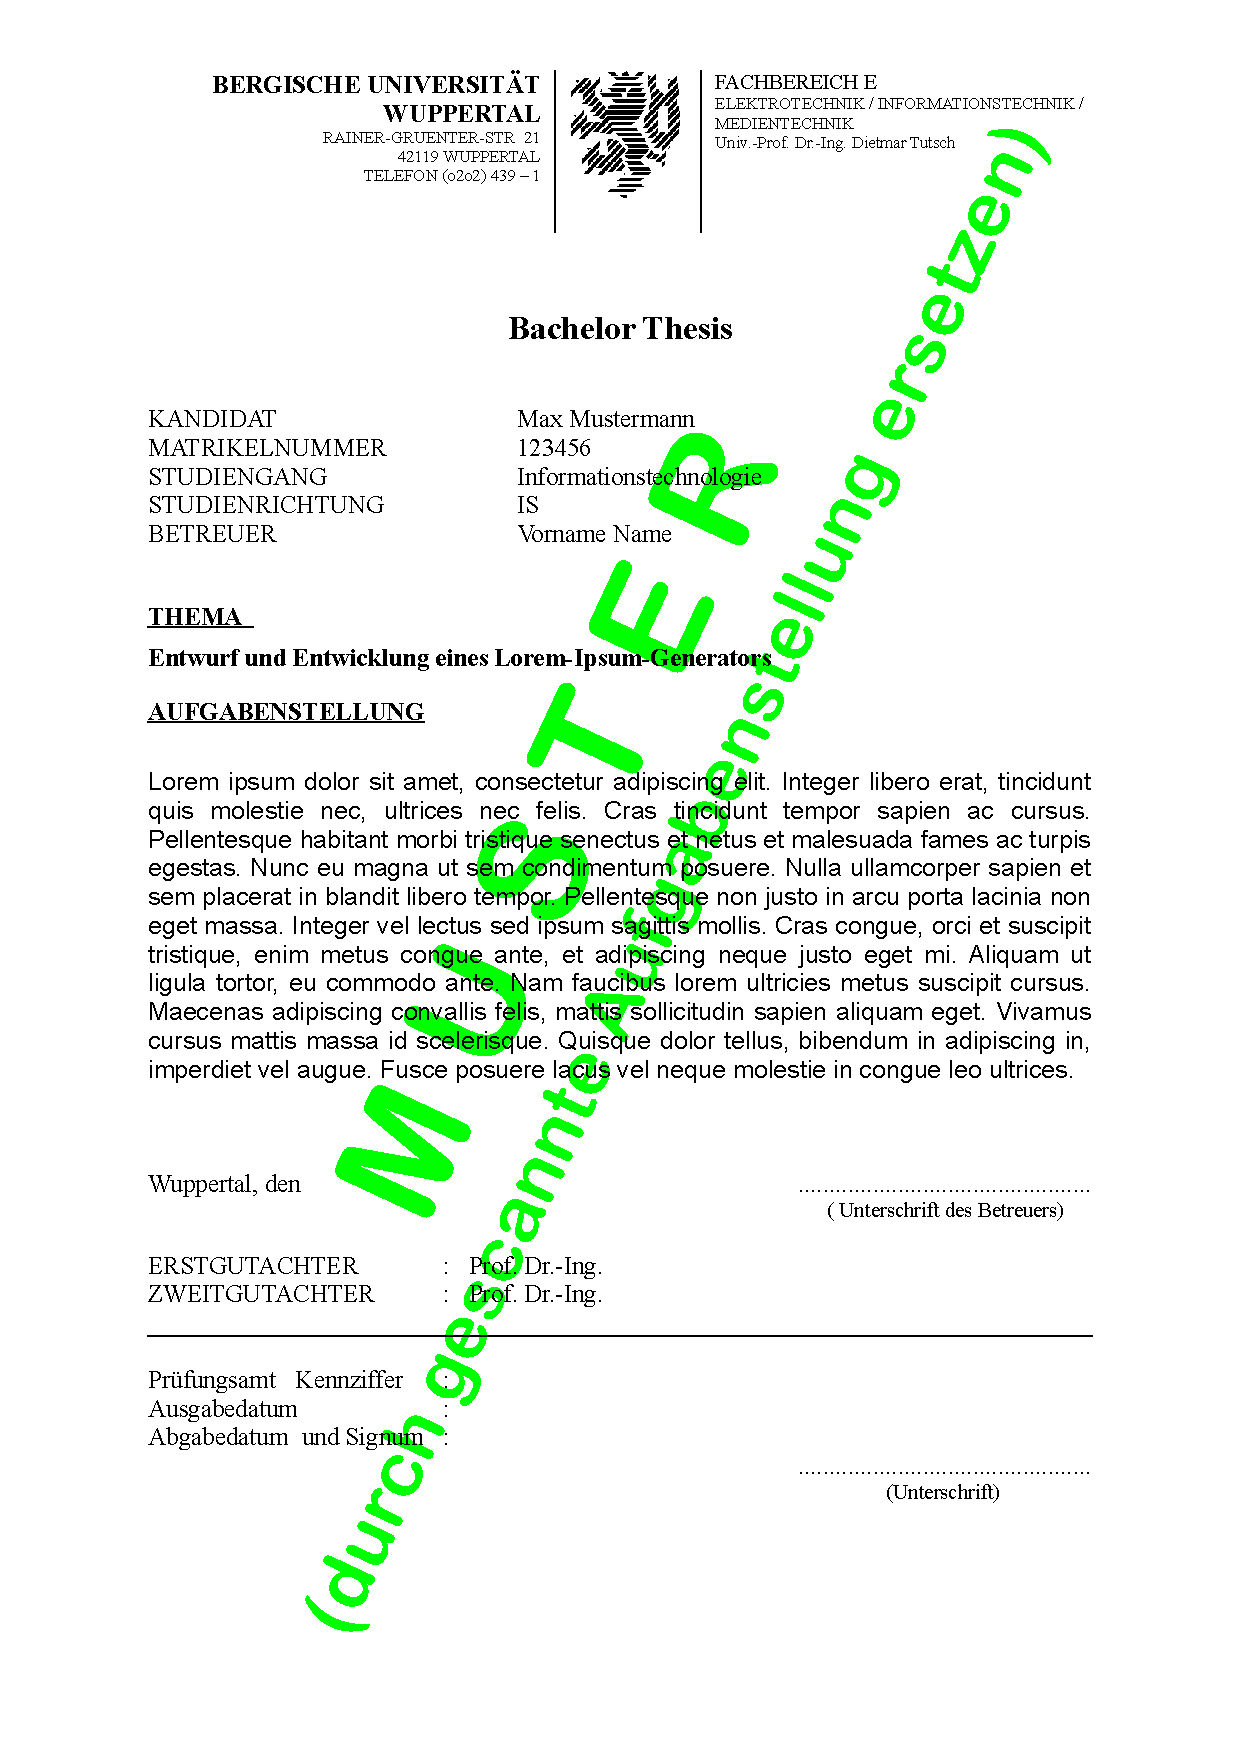
\includepdf[
		%pages={1},
		%fitpaper=true
	%]{Medien/Aufgabenstellung.pdf}%
	%\clearpage{\pagestyle{empty}\cleardoublepage}%
%
%
%%%%%%%%%%%%%%%%%%%%%%%%%%%%%%%%%%%%%%%%%%%%%%%%%%%%%%%%%%%%%%%%%%%%%%%%%%%%%%%%
%%% Verlängerung %%%%%%%%%%%%%%%%%%%%%%%%%%%%%%%%%%%%%%%%%%%%%%%%%%%%%%%%%%%%%%%
%
	%\ifbool{verlaengerung}{%
		%\cleardoublepage%
		%\pdfbookmark[1]{Verlängerung}{verlaengerung}%
		%
\includepdf[pages={1},fitpaper=true]{Medien/Verlaengerung.pdf}%
	  	%\clearpage{\pagestyle{empty}\cleardoublepage}%
	%}{}%
%
%
%%%%%%%%%%%%%%%%%%%%%%%%%%%%%%%%%%%%%%%%%%%%%%%%%%%%%%%%%%%%%%%%%%%%%%%%%%%%%%%%
%%% Erklärungen %%%%%%%%%%%%%%%%%%%%%%%%%%%%%%%%%%%%%%%%%%%%%%%%%%%%%%%%%%%%%%%%
%
	\pdfbookmark[1]{Erklärungen}{erklaerung}%
	\vspace*{2em}%
	
	\vspace*{\fill} % Push content to the vertical center
\begin{center}
    \Huge
    \textbf{If you fail, never give up because FAIL means ``First Attempt in Learning.''}
    
    \vspace{0.5cm}
    \hrule % Horizontal line
    \vspace{0.5cm}
    \large
    (APJ Abdul Kalam)
\end{center}
\vspace*{\fill} % Push content to the vertical center
	\newpage
	\section*{Declaration of Authorship}


\vspace{20pt}

I, Jay Karippacheril Jacob, declare that this thesis titled, "Accelerating the computation of the matrix sign function" and the work presented in it are my own. I confirm that:

\vspace{10pt}

\begin{itemize}
	
	\item This work was been done wholly or mainly while in candidature for a research degree at this University.
	\item Where any part of this thesis has previously been submitted for a degree or any other qualification at this University or any other institution, this has been clearly stated.
	\item Where I have consulted the published work of others, this is always clearly attributed.
	\item Where I have quoted from the work of others, the source is always given. With the exception of such quotations, this thesis is entirely my own	work.
	\item  I have acknowledged all main sources of help.
	\item Where the thesis is based on work done by myself jointly with others, I have made clear exactly what was done by others and what I have contributed myself.
	
\end{itemize}

\vspace{40pt}

\ifbool{zusatzErklaerung}{\vfill}{\vspace{4em}}%
\begin{tabular}{lc}%
	\ort, \abgabedatum \hspace*{1cm}& \rule[2px]{5cm}{0.5px}\\%
	&\footnotesize{(Signature)}%
\end{tabular}
\ifbool{zusatzErklaerung}{\vfill}{\vspace{5em}}%
	
	\newpage
	\section*{Acknowledgment}

First and foremost, I would like to express my heartfelt gratitude to Prof. Dr. Andreas Frommer. From the very first email inquiring about the possibility of working under his supervision to every step throughout the course of this thesis, he has been consistently kind, generous, and supportive. I deeply appreciate his guidance in helping me grasp the critical concepts required for my research and his invaluable assistance in rectifying the mistakes I made along the way. Our weekly meetings were always constructive, enlightening, and filled with engaging discussions, which I truly cherished. It has been a remarkable experience to complete my thesis under his supervision, and I am sincerely grateful for the initial ideas and references he provided that shaped the foundation of this work.

\vspace{10pt}

I am also deeply grateful to Dr. Gustavo Alonso Ramirez Hidalgo for his exceptional support and guidance. At the early stages of my thesis, I found certain technical concepts challenging to understand, but his clear explanations helped me navigate through these difficulties. I greatly appreciate the time and effort he invested in reviewing my algorithms and code, ensuring better implementations. Despite leaving the University of Wuppertal, he continued to offer his support, for which I will always be indebted. 

\vspace{10pt}

I would also like to extend my gratitude to Jose Jimenez Merchan for stepping in during the final stages of my thesis and offering guidance to me.

\vspace{10pt}

To Prof. Dr. Andreas Frommer, Dr. Gustavo Alonso Ramirez Hidalgo, and José Jiménez Merchán, I am immensely thankful for their unique personalities, unwavering support, and the time they dedicated to me throughout my master's thesis journey.

\vspace{10pt}

Lastly, I would like to express my heartfelt appreciation to my family, friends, and the Faculty of Mathematics and Natural Sciences at the University of Wuppertal. Their constant encouragement, support, and belief in me have been a source of strength throughout my master’s journey.

\vspace{20pt}

Thank you all for being an integral part of this significant milestone in my life.

	\newpage
	\section*{Abstract}

The matrix sign function arises in computations in lattice QCD. We look at the computation of the action $\text{sign}(Q)x$ of the sign function of the matrix $Q$ on a vector $x$. In our application, $Q$ is the symmetrized Wilson-Dirac operator. This is a Hermitian matrix if the chemical potential is 0; otherwise, it is non-Hermitian. Actually, we will always consider the inverse square root function, since $\text{sign}(Q)x = (Q^2)^{-1/2}Qx$.

The Arnoldi Krylov subspace approximation is the basis method to approximate $\text{sign}(Q)x$. There are several ways to accelerate the convergence of this basic scheme:
\begin{enumerate}
    \item \textbf{Restarts} (in the non-Hermitian case). This avoids having too many inner products in the Arnoldi orthogonalization.
    \item \textbf{Deflation} (explicit and implicit). This makes the matrix better conditioned and thus reduces the number of iterations. Explicit deflation uses the smallest left and right eigenvectors; implicit deflation is present in the thick restart approach of Eiermann and Güttel; see also the \texttt{funm} Matlab code.
    \item \textbf{Polynomial preconditioning.} This also makes the matrix better conditioned and thus reduces the number of iterations. A recent paper on this was published along with the numerical results for QCD on a parallel machine.
    \item \textbf{Sketching.} This is a randomized approach where we save orthogonalizations and sketch the Arnoldi matrix. The relevant paper is by Güttel and Schweitzer.
\end{enumerate}

\textbf{The purpose of the thesis} is to consider the following combination of the above approaches:
\begin{itemize}
    \item $2 + 1$ (as is already done in \texttt{funm})
    \item $2 + 3$ (building on existing work and code of Gustavo)
    \item $2 + 4$ (this is new, but Stefan Güttel just gave a talk on it at a conference in Paris)
\end{itemize}

\textbf{Tasks:}
\begin{enumerate}
    \item Understand and describe the individual methods (1--4).
    \item Describe, formulate algorithmically, and discuss the combined methods ($2+1$, $2+3$, $2+4$).
    \item Test the combined methods, in Matlab on small configurations.
\end{enumerate}





%
%
%%%%%%%%%%%%%%%%%%%%%%%%%%%%%%%%%%%%%%%%%%%%%%%%%%%%%%%%%%%%%%%%%%%%%%%%%%%%%%%%
%%% Danksagung %%%%%%%%%%%%%%%%%%%%%%%%%%%%%%%%%%%%%%%%%%%%%%%%%%%%%%%%%%%%%%%%%
	%\ifbool{danksagung}{%
		%\vspace*{\fill}\vspace{-3em}%
		%\pdfbookmark[1]{Danksagung}{danksagung}%
		%\section*{Danksagung}
\todo{Text der Danksagung wird hier eingetragen.}

Lorem ipsum dolor sit amet, consectetur adipiscing elit. Integer libero erat, tincidunt quis molestie nec, ultrices nec felis. Cras tincidunt tempor sapien ac cursus. Pellentesque habitant morbi tristique senectus et netus et malesuada fames ac turpis egestas. Nunc eu magna ut sem condimentum posuere. Nulla ullamcorper sapien et sem placerat in blandit libero tempor. Pellentesque non justo in arcu porta lacinia non eget massa. Integer vel lectus sed ipsum sagittis mollis. Cras congue, orci et suscipit tristique, enim metus congue ante, et adipiscing neque justo eget mi. Aliquam ut ligula tortor, eu commodo ante. Nam faucibus lorem ultricies metus suscipit cursus. Maecenas adipiscing convallis felis, mattis sollicitudin sapien aliquam eget. Vivamus cursus mattis massa id scelerisque. Quisque dolor tellus, bibendum in adipiscing in, imperdiet vel augue. Fusce posuere lacus vel neque molestie in congue leo ultrices.%
		%\vfill%
	%}{}
%
%
%%%%%%%%%%%%%%%%%%%%%%%%%%%%%%%%%%%%%%%%%%%%%%%%%%%%%%%%%%%%%%%%%%%%%%%%%%%%%%%%
%%% Kurzfassung & Abstract %%%%%%%%%%%%%%%%%%%%%%%%%%%%%%%%%%%%%%%%%%%%%%%%%%%%%
%
	%\clearpage{\pagestyle{empty}\cleardoublepage}
	%\vspace*{\fill}\vspace{-3em}
	%\pdfbookmark[1]{Kurzfassung}{kurzfassung}
	%%% Version 2023-08-21
%% LaTeX-Vorlage für Abschlussarbeiten
%% Erstellt von Nils Potthoff, ab 2020 erneuert und ausgebaut von Simon Lohmann
%% Lehrstuhl Automatisierungstechnik/Informatik Bergische Universität Wuppertal
%%%%%%%%%%%%%%%%%%%%%%%%%%%%%%%%%%%%%%%%%%%%%%%%%%%%%%%%%%%%%%%%%%%%%%%%%%%%%%%%

% INFO: Die Kurzfassung wird immer auf Deutsch UND Englisch benötigt!

% Kurzfassung auf Deutsch
\begingroup 
	\selectlanguage{ngerman}% der folgende Text ist auf Deutsch
	\section*{Kurzfassung}
	\todo{Der Text der Kurzfassung wird hier eingetragen.}
	\blindtext
\endgroup

% Kurzfassung auf Englisch
\begingroup
	\selectlanguage{english}% der folgende Text ist auf Englisch
	\section*{Abstract}
	\todo{The english version.}
	\blindtext
\endgroup

	\vfill
	\clearpage
%
%
%%%%%%%%%%%%%%%%%%%%%%%%%%%%%%%%%%%%%%%%%%%%%%%%%%%%%%%%%%%%%
%  INHALTSVERZEICHNIS
\markboth{\contentsname}{}
\pdfbookmark[1]{\contentsname}{toc}
\begingroup
	\renewcommand{\markboth}[2]{}{}
	\tableofcontents
\endgroup
\clearpage
%
%
%%WIDMUNG, VORWORT
%
%% Ende der Titelei; es folgt der Hauptteil
\ifbool{doppelseitig}{%
	\clearpage%
	\hphantom{anker, damit hier auch wirklich eine leere Seite ist}%
}{}%
{\pagestyle{empty}\cleardoublepage}% Inhalt soll auf rechter Seite beginnen
\pagenumbering{arabic}%
\pagestyle{thesis-page-regular}%

 % Titelseite etc. (bitte nicht ändern) %%%%%%%%%
	%%%%%%%%%%%%%%%%%%%%%%%%%%%%%%%%%%%%%%%%%%%%%%%%%%%%%%%%%%%%%%%%%%%%%%%%%%%%
	%%%%%%%%%%%%%  Ab hier ändern und ergänzen  %%%%%%%%%%%%%%%%%%%%%%%%%%%%%%%%
	%%%%%%%%%%%%%  | | | | | | | | | | | | | |  %%%%%%%%%%%%%%%%%%%%%%%%%%%%%%%%   
	%%%%%%%%%%%%%  V V V V V V V V V V V V V V  %%%%%%%%%%%%%%%%%%%%%%%%%%%%%%%%
	\chapter{Introduction}
\label{sec: intro}

% Introduction to matrix functions and their applications.
Consider a matrix $\mathbf{A} \in \mathbb{C}^{n \times n}$, a vector $\mathbf{b} \in \mathbb{C}^{n}$ and a function $\mathbf{f} : \mathbb{C} \to \mathbb{C}$, the action of a matrix is defined as:
\begin{equation}
    f(A)b
    \label{eq:1.1}
\end{equation}
The above expression represents a product of the matrix function $f(A) \in \mathbb{C}^{n \times n}$ on a vector \textbf{b}. There exists a huge interest in the action of a matrix on a vector in the fields of science and engineering.
Some of the most interesting cases widely under studies are :
\begin{enumerate}
    \item \textbf{Matrix exponential function}  $f(z) = e^z$, forms the core of exponential integrators used for solving differential equations \cite{1,2,3}. 
    \item \textbf{Matrix square root} $f(z) = z^{1/2}$, in machine learning \cite{6} and in other domains such as image processing, advection-diffusion problems, elasticity and many more \cite{4,5}.
    \item \textbf{Matrix logarithm} $f(z) = \log(z)$, used in Markov model analysis \cite{7}.
    \item \textbf{Matrix fractional powers} $f(z) = z^\alpha$, in fractional differential equations \cite{9}.
    \item \textbf{Matrix sign function} $f(z) = \sgn(z)$, in lattice quantum chromodynamics (QCD) \cite{11, 10}.
\end{enumerate}
The most straightforward approach to compute $f(A)\mathbf{b}$ is to first calculate $f(A)$ and then perform matrix multiplication with $\mathbf{b}$. However, as the dimension of the matrix grows, this approach becomes impractical due to various reasons such as the storage complexity, computational cost of matrix functions, and inefficiency of matrix-vector multiplication.

%%%%%%%%%%%%%%%%%%%%%%%%%%%%%%%%%%%%%%
%% Add a sentence explaining the reasons.
%%%%%%%%%%%%%%%%%%%%%%%%%%%%%%%%%%%%%%

% Brief QCD lattice computation and the type of matrices we are dealing with.
Here, our domain of interest is the matrix sign function, in conjunction with the application of lattice QCD. The most significant challenge faced in lattice QCD was the implementation of chiral symmetry on the lattice \cite{12} and one among the prominent solutions proposed to overcome this was the Overlap-Dirac operator involving the sign function, which avoids low mode calculation for chiral symmetry \cite{13}. However, the drawback of the above proposal was the huge computational cost of the matrix sign function since the matrix $A$ is a large sparse matrix. Typically the matrix $A$ is Hermitian and efficient methods have been already developed to approximate them as mentioned in papers \cite{14,10}.

Studying the relativistic heavy ion collisions theoretically in lattice simulations and model calculations implies presenting a non-zero density. As a result, a quark chemical potential is introduced to the QCD Lagrangian, leading to the loss of hermiticity of the matrix $A$ as in \cite{16}. Therefore, we are now faced with the computation of the explained matrix sign function for a non-Hermitian matrix $A$. Furthermore, it is to be highlighted that we will always consider the inverse square root function, since $\text{sign}(Q)x = (Q^2)^{-1/2}Qx$, which would be further detailed in the following chapters.

% How to solve these kinds of problems and the problems present in them
For smaller lattices, the existing methods could be used in the above-mentioned problem. However, as the dimension of the matrix becomes larger, one has to heavily depend upon iterative methods for approximating the matrix sign function. Some of the popular methods under use in such situations are polynomial \cite{17,18} and rational \cite{19,20,21} Krylov methods which demand a high arithmetic cost for the orthogonalization of a Krylov basis or a large memory cost for the storage of Krylov basis vectors. These limitations narrow down the attainable accuracy of the Krylov methods. To address these constraints, there are several strategies available. Among them a few strategy of interest that could accelerate the convergence are:
\begin{enumerate}
    \item \textbf{Restarts} (in the non-Hermitian case). This avoids having too many inner products in the Arnoldi orthogonalization \cite{52}.
    \item \textbf{Deflation} (explicit and implicit). This makes the matrix better conditioned and thus reduces the number of iterations. Explicit deflation uses the smallest left and right eigenvectors; \cite{52, 11}.
    \item \textbf{Polynomial preconditioning.} This also makes the matrix better conditioned and thus reduces the number of iterations \cite{49}.
    \item \textbf{Sketching.} This is a randomized approach where we save orthogonalizations and sketch the Arnoldi matrix \cite{41}.
\end{enumerate}

% Brief on what is being discussed and analysed in this thesis
In this thesis, we explore new possibilities arising from the combination of deflation and Krylov subspace methods based on the above strategies, chosen for their strengths in relation to the matrix sign function and specific applications of interest. In Chapter \ref{sec:matrix_fun}, we begin with an introduction to matrix functions, including essential definitions and properties. This discussion narrows in Chapter \ref{sec:matrix_sign_func}, where we focus on the matrix sign function, our primary area of investigation. Here, we cover definitions and properties derived from matrix functions, along with specific characteristics unique to the matrix sign function.

We indicated that our interest are in large non-Hermitian matrices of dimension $N$. Hence, in chapter \ref{sec:QCD_sim_and_non_herm_challenges} provides a concise overview of Quantum Chromodynamics (QCD) simulations, particularly the Wilson-Dirac and overlap operators in lattice QCD. We examine the limitations encountered in calculating sign functions in this context, highlighting the challenges and the motivation to develop algorithms that enhance efficiency and stability.

Our goal is to approximate the action of a matrix sign function on a vector more efficiently and stably. To this end, we introduce recent methods identified in our literature review, alongside algorithms for their implementation, in Chapters \ref{sec:kryl_subspace_app} and \ref{sec:deflation}. In Chapter \ref{sec:expl_poss}, we present a framework for implementing potential new algorithms and discuss the rationale behind the choices and combinations selected for our numerical experiments. Finally, Chapter \ref{sec:num_exper} provides an in-depth analysis of the performance of these algorithms across various parameters.
	\chapter{Matrix Functions}
\label{sec:matrix_fun}

% It provides a brief overview of what we will discuss in this section.
As a starting point for this thesis, we begin our research by reviewing the existing literature on our domain of interest, the action of a matrix $f(A)\mathbf{b}$. Specifically, we are focused on algorithms that can expedite the matrix sign functions, $sgn(A)$ for large non-Hermitian matrices with dimension $N$.To achieve this objective, we begin by presenting fundamental information on matrix functions. This is followed by a discussion of the matrix sign function in Chapter \ref{sec:matrix_sign_func}. 

In the prior Chapter, we indicated our interest in large non-Hermitian matrices of dimension $N$. Hence, with the help of chapter \ref{sec:QCD_sim_and_non_herm_challenges}, we will elucidate the reason behind the focus on this particular class of matrices. Proceeding further in this review, we aim to address algorithms that could potentially minimize the two significant computational challenges: cost and time. Chapter \ref{sec:kryl_subspace_app} introduces Krylov methods, including the Arnoldi method, the restarted Arnoldi method, and the sketched Arnoldi method, which are of particular interest for further research. Chapter \ref{sec:deflation} will explore deflation along with the LR-deflation algorithm, another area of keen interest.

% A small introduction to start on the topic matrix functions
Throughout this Chapter, we will anchor our discussion on \cite{8}, which provides a robust foundation for the theory of matrix functions. As outlined in this reference, although there exist different ways of defining $f(A)$ there are three definitions we are interested in the context of computing $f(A)$.

\section{Definitions of \emph{$f(A)$}}
\label{sec:def_f(A)}

% In this subsection we will introduce the general definitions for the action of a matrix.

\begin{definition}
    \label{def:2.1}
    \cite{8}(Jordan canonical form). Any matrix $A \in \mathbb{C}^{n \times n}$ can be written in the Jordan canonical form,

    \begin{align}
        Z^{-1} A Z &= J = \text{diag}(J_1, J_2, \ldots, J_p),
        \label{eq:2.1}
    \end{align}

    \begin{align}
        J_k &= J_k(\lambda_k) = \begin{bmatrix}
        \lambda_k & 1 & & \\
        & \lambda_k & \ddots & \\
        & & \ddots & 1 \\
        & & & \lambda_k
        \end{bmatrix} \in \mathbb{C}^{m_k \times m_k}.
        \label{eq:2.2}
    \end{align}
    where $Z$ is non-singular and $m_1 + m_2 + ... + m_p = n$.
\end{definition}

In the above standard result, the Jordan matrix $J$ is unique up to the ordering of the blocks $J_i$, whereas $Z$ known as the transforming matrix is not unique. Here, $\lambda_1,...,\lambda_p$ denotes the distinct eigenvalues of the matrix $A$ used to formulate Jordan blocks, with $n_i$ representing the size of the largest Jordan block containing eigenvalue $\lambda_i$.

Before presenting the definition of matrix functions via Jordan canonical form, we first introduce the following terminology.

\begin{definition}
    \label{def:2.2}
    \cite{8}The function $f$ is said to be defined on the spectrum of A if the values
    \[
        f^{(j)}(\lambda_i), \quad j=0:n_i-1, \quad i=1:s
    \]
    exist. These are called the values of the function f on the spectrum of A.
\end{definition}

The following definition of matrix functions via the Jordan canonical form depends solely on the values of $f$ evaluated at the spectrum of $A$, without requiring additional information beyond this spectrum. Indeed, any $\sum_{i=1}^s n_i$ arbitrary values can be chosen and assigned as the values of $f$ on the spectrum of $A$. Only when making statements about global properties, such as continuity, do we need to impose additional assumptions on $f$.

\begin{definition}
    \label{def:2.3}
    \cite{8}(matrix function via Jordan canonical form). Let $f$ be defined on the spectrum of $A \in \mathbb{C}^{n \times n}$ and let $A$ have the Jordan canonical form \ref{eq:2.1} and \ref{eq:2.2}. Then
    \begin{equation}
        f(A) := Zf(J)Z^{-1} = Z \mathrm{diag}(f(J_k))Z^{-1}
        \label{eq:2.3}
    \end{equation}
    where
    \begin{equation}
        f(J_k) :=
        \begin{bmatrix}
            f(\lambda_k) & f'(\lambda_k) & \cdots & \frac{f^{(m_k-1)}(\lambda_k)}{(m_k-1)!} \\
            & f(\lambda_k) & \ddots & \vdots \\
            & & \ddots & f'(\lambda_k) \\
            & & & f(\lambda_k)
        \end{bmatrix}
        \label{eq:2.4}
    \end{equation}.
\end{definition}

The insights we infer from the first definition for $f(A)$ are:
\begin{enumerate}
    \item $f(A)$ is independent of the Jordan canonical form used.
    \item If $A$ is diagonalizable then the Jordan canonical form reduces to an eigendecomposition $A=ZDZ^{-1}$, with $D=diag(\lambda_i)$ and the columns of $Z$ are eigenvectors of $A$
    \end{enumerate}
    
The Jordan canonical form is rarely used in computations due to its high sensitivity to perturbations. However, in the special case where \( A \) is normal (i.e., unitarily diagonalizable), the second inference from the aforementioned definition becomes applicable and $f(A)$ could be computed from the well-conditioned eigendecomposition. This direct method of computing $f(A)$ is therefore employed only when $A$ is a small Hermitian matrix, with a computational complexity of \( O(n^3) \) \cite{8}. 

The second approach for defining $f(A)$ is with the help of polynomial interpolation, which yields numerous useful properties.

\begin{theorem}
    \label{the:2.4}
    \cite{8}For polynomials $p$ and $q$ and $A \in \mathbb{C}^{n \times n}$, $p(A) = q(A)$ if and only if $p$ and $q$  take the same values on the spectrum of A.
\end{theorem}

The above theorem establishes that the matrix $p(A)$ is entirely determined by the values of $p$ on the spectrum of $A$.

\begin{definition}
    \label{def:2.5}
    \cite{8}(matrix function via Hermitian interpolation). Let $f$ be defined on the spectrum of $A \in \mathbb{C}^{n \times n}$ and let $\psi$ be the minimal polynomial of $A$, where $\psi(x)=\prod^{s}_{i=1}(x-\lambda_{i})^{n_{i}}$ Then $f(A) := p(A)$, where $p$ is the polynomial of degree less than
    \[
        \sum_{i=1}^{s} n_i = \deg \psi
    \]
    that satisfies the interpolation conditions
    \begin{equation}
        p^{(j)}(\lambda_i) = f^{(j)}(\lambda_i), \quad j=0:n_i-1, \quad i=1:s
        \label{eq:2.5}
    \end{equation}

    There is a unique such $p$ with minimal degree and it is known as the Hermite interpolation polynomial.
\end{definition}

While the second definition of $f(A)$ appears more numerically practical than the first, it is important to note that the interpolating polynomial $p$ not only depends on $f$ but also on the eigenvalues of $A$. As cited in \cite{15}, it would necessitate $O(n^{4} )$ floating point operations ($(O(n)$ matrix-matrix multiplications each of which costs $O(n^{3} )$) to produce $f(A)$ and is numerically unstable.

\begin{remark}
    \label{rem:2.6}
    Some important remarks on the above definition based on \cite{8}are:
    \begin{enumerate}
    \item If the polynomial $q$ satisfies the interpolation conditions specified in Equation \ref{eq:2.5} as well as additional interpolation conditions (whether at the same or different $\lambda_i$), then $q$ and the polynomial  $p$ from Definition \ref{def:2.5} yield identical values on the spectrum of $A$. Consequently, by Theorem \ref{the:2.4}, it follows that $q(A) = p(A) = f(A)$.

    \item The Hermite interpolating polynomial $p$ can be defined explicitly by the Lagrange–Hermite formula

    \begin{equation}
        p(t) = \sum_{i=1}^{s} \left[ \left( \sum_{j=0}^{n_{i}-1} \frac{1}{j!} \phi_{i}^{(j)}(\lambda_{i})(t-\lambda_{i})^{j} \right) \prod_{\substack{j=1 \\ j \neq i}}^{s} (t-\lambda_{j})^{n_{j}} \right]
        \label{eq:2.6}
    \end{equation}
    where  $\phi_i(t) = \frac{f(t)}{\prod_{j \neq i} (t - \lambda_j)^{n_j}}$.

    \item The definition explicitly makes $f(A)$ a polynomial in $A$.

    \item According to Definition \ref{def:2.5}, even if $f$ is represented by a power series, $f(A)$ can still be expressed as a polynomial in $A$ of degree at most $n-1$.

    \item If $A$ is a real, diagonal matrix, then for the condition  $f(A)$ to be real whenever $A$ is real becomes evident only when the scalar function $f$ is real on the subset of the real line on which it is defined.

    \item The Definition \ref{def:2.5} could be directly derived from the formula mentioned in equation \ref{eq:2.4} for a function of the Jordan block $J_k$. 
    We can directly derive from Definition \ref{def:2.5} the formula \ref{eq:2.4} for a function of the Jordan block $J_k$. The sufficient interpolation conditions to achieve the Hermite interpolating polynomial,
    \[
        p(t) = f(\lambda_k) + f'(\lambda_k)(t - \lambda_k) + \frac{f''(\lambda_k)}{2!}(t - \lambda_k)^2 + \cdots + \frac{f^{(m_k-1)}(\lambda_k)}{(m_k-1)!}(t - \lambda_k)^{m_k-1}.
    \]

    \end{enumerate}
\end{remark}

The third approach of defining $f(A)$ involves the Cauchy integral theorem, assuming $f$ is analytic, unlike the other two definitions where $f$ has to be defined on the spectrum of $A$.

\begin{definition}
    \label{def:2.7}
    \cite{8}(matrix function via Cauchy integral). For $A \in \mathbb{C}^{n \times n}$,

    \begin{equation}
        f(A) := \frac{1}{2\pi i} \int_\Gamma f(z)(zI - A)^{-1}dz
        \label{eq:2.7}
    \end{equation}
    where $f$ is analytical on and inside a closed contour $\Gamma$ that encloses $spec(A)$.
\end{definition}

The above definition is highly applicable to our problem of interest. Here we face many numerical challenges and the most critical challenge encountered is the identification of an appropriate contour $\Gamma$ and a quadrature rule that depends on both $f$ and $A$.

Thus, a good definition is one that can be chosen to not only yield the expected properties but also reveal useful, less obvious ones. Accordingly, we conclude this chapter by presenting some general properties derived from the definition of $f(A)$.

\begin{remark}
\label{rem:2.8}
    (properties of the matrix functions)\cite{8}
    \begin{enumerate}
        \item $f(A)$ commutes with A.
        \item $f(A^{T})=f(A)^{T}$.
        \item $f(XAX^{-1})=Xf(A)X^{-1}$.
        \item The eigenvalues of $f(A)$ are $f(\lambda_{i})$, where the $\lambda_{i}$ are the eigenvalues of $A$.
        \item If $X$ commutes with $A$ then $X$ commutes with $f(A)$.
    \end{enumerate}
\end{remark}
	\chapter{Matrix Sign Function}
\label{sec:matrix_sign_func}

% An introduction to what a scalar sign function is!
To introduce the matrix sign function, it is essential to explore the scalar sign function as it represents an extension of their scalar counterparts. The scalar sign function is defined over the complex plane excluding the imaginary axis: $\mathbb{C}\setminus\mathbb{C}^0 = \mathbb{C}^+ \cup \mathbb{C}^-$ where $\mathbb{C}^-$, $\mathbb{C}^+$ and $\mathbb{C}^0$ denote the open right-half complex plane, the open left-half complex plane, and the imaginary axis, respectively. Thus, the scalar sign function for $z \in \mathbb{C}^+ \cup \mathbb{C}^-$ is defined by\cite{22}

\begin{equation}
    \sgn z = \begin{cases}
                1, & z \in \mathbb{C}^+ \\
                -1, & z \in \mathbb{C}^-
            \end{cases}.
            \label{eq:2.8}
\end{equation}

The above definition implies that if $z \in \mathbb{C}^{\theta} = \{iy, y \in \mathbb{R}\}$ then $\sgn(z)$ is undefined. Now based on the above, to define the matrix sign function, we proceed under the assumption that $A \in \mathbb{C}^{n \times n}$ does not possess eigenvalues lying on the imaginary axis, thereby ensuring $A$ is non-singular and $\sgn(A)$ remains well-defined. These conditions are crucial for establishing the validity of $\sgn(A)$. There exist numerous equivalents for matrix sign functions that extend meaningful insights into the properties they possess. In the following subsection, we will examine several pertinent definitions essential to this thesis.

\section{Definition of \emph{$\sgn(A)$}}
\label{sec:def_sgn(A)}

% In this subsection we will introduce the general definitions for the matrix sign function.
\begin{definition}
    \label{def:2.8}
    \cite{23}(Jordan canonical form) Let the matrix $A$ have a Jordan decomposition
    
    \[
        A=T\begin{bmatrix}
            N&0\\ 
            0&P
        \end{bmatrix}T^{-1},
    \]
    where $N$ and $P$ are square matrices with eigenvalues in $\mathbb{C}^-$ and $\mathbb{C}^+$, respectively. Then the sign of $A$ is defined to be,

    \begin{equation}
        \sgn(A)=T\begin{bmatrix}
            -I_{N}&0\\ 
            0&I_{P}
        \end{bmatrix}T^{-1},
        \label{eq:2.9}
    \end{equation}
    where the identity matrices $I_{N}$, and $I_{P}$, are compatibly dimensioned with $N$ and $P$, respectively.

\end{definition}
The above definition is a derivation of Definition \ref{def:2.3}, where the matrix function is the sign function, and for this function, all derivatives of all orders are zero.

Some intriguing properties for $\sgn(A)$ derived from the above initial definition are highlighted in the following remark.

\begin{remark}
\label{rem:2.9}
    (properties of the sign function)\cite{22, 23}
    \begin{enumerate}
        \item $\sgn(A)$ is diagonalizable with eigenvalues equal to $\pm1$.
        \item $\sgn(A)^2 = I$.
        \item  If $c$ is a nonzero real scalar, then $\sgn(cA)=\sgn(c)\sgn( A)$.
        \item $\nega(A) \equiv (I-\sgn(A))/2$ is a projection onto the negative invariant subspace of $A$ and $\posi(A) \equiv (I+\sgn(A))/2$ is a projection onto the positive invariant subspace of $A$, where the positive and negative invariant subspaces of $A$ are the subspaces corresponding to the eigenvalues of $A$ in $\mathbb{C}^-$ and $\mathbb{C}^+$ respectively.
    \end{enumerate}
\end{remark}

\begin{lemma}
    \label{lem:2.10}
    \cite{22}Given,
    
    \[
        A=U\begin{bmatrix}
            N&T\\ 
            0&P
        \end{bmatrix}U^{T},
    \]
    where $U$ is an orthogonal matrix, $N$ has eigenvalues in $\mathbb{C}^-$, and $P$ has eigenvalues in $\mathbb{C}^+$. Then the sign of $A$ is given by,

   \begin{equation}
        sgn(A)=U\begin{bmatrix}
            -I_{N}&S\\ 
            0&I_{P}
        \end{bmatrix}U^{T},
        \label{eq:2.10}
   \end{equation}
    where $S$ satisfies the Sylvester equation,
    \begin{equation}
        NS - SP = -2T.
        \label{eq:2.11}
    \end{equation}

\end{lemma}

The above formulation proves to be highly beneficial. It can be used to analyze the stability of Newton iteration \cite{24, 25} and analyze the conditioning \cite{25} of the matrix sign function. This definition further serves as a foundation for a method of solving the stable Sylvester equation of the form \eqref{eq:2.11}. In the equation \eqref{eq:2.10} replace $U$ with $I$ to determine $\sgn(A)$. Now, the upper right block which is $S$ of $\sgn(A)$ is the solution desired to be found from the above-stated Sylvester equation.

The second type of definition is based on integral representations. Utilizing a residue argument, presented in the spectral theory of operators, Robert derives an integral formula of the form \cite{23},

\begin{equation}
    \posi(A) = \frac{1}{2 \pi i} \int_{D} (\zeta I - A)^{-1} d\zeta,
    \label{eq:2.12}
\end{equation}
where $D$ is a simple closed contour in $\mathbb{C}^{+}$ containing the eigenvalues of $A$ with positive real part and pos(A) as mentioned in remark \ref{rem:2.9}. From this equation and the remark \ref{rem:2.9} Robert derived an integral representation as a definition for $\sgn(A)$,

\begin{definition}
    \label{def:2.11}
   \begin{equation}
        \sgn(z) = \frac{2}{\pi}z\int_{0}^{+\infty}(y^{2}I+z^{2})^{-1}dy.
        \label{eq:2.13}
    \end{equation} 
\end{definition}
    
Definition \ref{def:2.7} and the above definition are identical when $f(z) \equiv 1$ for the contour $\mathcal{C}^+$ in Definition \ref{def:2.7}. 

The third method of defining $\sgn(A)$ is through matrix iterations. Newton's iteration is the most popular iterative method to find $\sgn(A)$. The method is applied to the equation $S^{2}-I=0$. Let $A_{0} = A_k$ and set

\begin{equation}
    A_{k+1}=\frac{1}{2}(A_{k}+A_{k}^{-1}).
    \label{eq:2.15}
\end{equation}

The above matrix iteration is globally convergent for all matrices $A$ with eigenvalues in $\mathbb{C}^{-} \cup \mathbb{C}^{+}$.

\begin{equation}
    sgn(A) = \lim_{k\longrightarrow+\infty}A_{k}.
    \label{eq:2.16}
\end{equation}

An intriguing aspect of Newton's iterative method is that the convergence is quadratic when $A_k$ is close to the actual $\sgn(A)$ but could be relatively slow at the initial stages.

Higher-order Padé iterative methods are another form of iterative methods used for the computation of $\sgn(A)$. The general form of the equation used in these iterations for order $n$ is,

\begin{equation}
    A_{k+l} = P_{n}(A_{k})Q_{n}^{-1}(A_{k}),
    \label{eq:2.17}
\end{equation}
where $P_{n}(A)$ and $Q_{n}(A)$ are the odd and even parts respectively of the polynomial $(I+A)^{n}$.The Padé iterations are globally convergent and serve as an implicit definition for $\sgn(A)$. Introduction of the $\tanh$ identity in equation \eqref{eq:2.17} helps in the study of chaotic behaviours of $\sgn(A)$ on the eigenvalues of $A$ close to the imaginary axis \cite{26}.

\begin{equation}
    P_{n}(A_{k})Q_{n}^{-1}(A_{k}) = \tanh(n\arctanh(A_{k})).
    \label{eq:2.18}
\end{equation}

If we represent $x$ in polar form, i.e., $x = r e^{i \phi}$, then $x$ has two principal branches, given by $\sqrt{x} = \pm\sqrt{r} e^{i \frac{\phi}{2}}$ for $\phi \in [-\pi, \pi]$. Following the first type of definition and extending the scalar formulation of the sign function, we define $\sgn(z) = \frac{z}{\sqrt{z^2}}$ as presented by Higham \cite{27} and apply it to the corresponding matrix function. This extension holds only when $z$ is not purely imaginary and consequently, when extended to a matrix $A$, the matrix must have no purely imaginary eigenvalues.

For such matrices, $A^2$ contains no eigenvalues on the negative real axis, thus ensuring that there exists a unique square root, $N=(A^{2})^{\frac{1}{2}}$. This commutes with $A$ and has eigenvalues in the open right-half complex plane as cited in the paper \cite{28}. Thus we have a definition for the matrix sign function:

\begin{definition}
    \label{def:2.12}
    Let $spec(A) \cap \mathbb{R}^{-} = \emptyset$, then 
    \begin{equation}
        \sgn(A) = A(A^2)^{-\frac{1}{2}}.
        \label{eq:2.19}
    \end{equation}
\end{definition}
	\chapter{QCD simulations and its Non-Hermitian challenges}
\label{sec:QCD_sim_and_non_herm_challenges}

% Intro. into QCD
One of the most demanding applications for supercomputers currently is Lattice QCD simulation, where a significant amount of resources are allocated. Quantum chromodynamics (QCD) is a quantum field theory for the strong interaction of the quarks via gluons \cite{30}. This theory is applied to make predictions on masses and resonance spectra on hadrons \cite{29}.

\section{The Wilson-Dirac and the overlap operator in lattice QCD}
\label{sec:wil_dirac_overlap}

% A Brief on the section in QCD where the problem originates.
The governing equation that determines the dynamics of the quarks and the interaction of quarks and gluons is the Dirac equation.

\begin{equation}
    D\psi + m \cdot \psi = \eta.
    \label{eq:2.20}
\end{equation}

In the above equation the quark fields are represented by $\psi = \psi(x)$ and $\eta = \eta(x)$, where $x$ denotes the points in space-time,
$x = (x_{0}, x_{1}, x_{2}, x_{3})$ \cite{31}. The Dirac operator $D$ in the equation \eqref{eq:2.20} represents the gluons and sets the mass of the quarks in the QCD theory. The parameter $m$ is a scalar mass. The Dirac operator can be written as:

\begin{equation}
    D = \sum_{\mu=0}^{3} \gamma_{\mu} \otimes (\partial_\mu + A_\mu),
    \label{eq:2.21}
\end{equation}
where $\partial_\mu = \partial / \partial x_{\mu}$ and $A$ is the gluon gauge field with the anti-hermitian traceless matrices $A_{\mu}(x)$. The $\gamma$-matrices represent the generators of the Clifford algebra \cite{32}. At a given point $x$, the quark field $\psi$ is expressed by a twelve-component column vector. These column vectors correspond to three colours and four spins, acted upon by $A_{\mu}(x)$ and $\gamma_{\mu}$ respectively.

To align with our study, we rewrite the massless overlap Dirac operator with a non-zero chemical potential $\mu$ as follows\cite{33}:

\begin{equation}
    D_{ov}(\mu) = 1+\gamma_{5}sgn(H_{w}(\mu)),
    \label{eq:2.22}
\end{equation}
where $H_{w}(\mu) = \gamma_{5}D_{w}(\mu)$, $D_{w}(\mu)$ is the Wilson-Dirac operator at nonzero chemical potential \cite{34, 35} with negative Wilson mass $m_{w} \in (-2, 0)$, $\gamma_{5} = \gamma_{1}\gamma_{2}\gamma_{3}\gamma_{4}$. The Wilson-Dirac operator is a discretization of the Dirac operator on a four-dimensioned lattice given as,

\begin{equation}
    \begin{aligned}
        \relax [D_w (\mu)]_{nm} = \delta_{n,m} \\ 
        &- \kappa \sum_{j=1}^{3} (1 + \gamma_j) U_{n,j} \delta_{n+\hat{j},m}- \kappa \sum_{j=1}^{3} (1 - \gamma_j) U_{n-\hat{j},j}^{\dagger} \delta_{n-\hat{j},m} \\
        &- \kappa (1 + \gamma_4) e^\mu U_{n,4} \delta_{n+\hat{4},m}- \kappa (1 - \gamma_4) e^{-\mu} U_{n-\hat{4},4}^{\dagger} \delta_{n-\hat{4},m},
    \end{aligned}
    \label{eq:2.23}
\end{equation}
where $\kappa = 1/(8+2m_{w})$ and $U_{n,v}$ is the \textit{SU}(3)-matrix associated with the link connecting the lattice site $n$ to $n + \hat{v}$. One of the most important highlights of the Wilson-Dirac operator is that compared to the naive discretization of the derivative operator, it avoids the replication of the fermion species for the continuum Dirac operator.

In the discretized formula \eqref{eq:2.23} the non-Hermiticity of the operator arises due to the term $e^{\pm \mu}$. The quark field at each lattice site corresponds to 12 variables: 3 \textit{SU}(3) colour components $\times$ 4 Dirac spinor components. This depicts that the matrix $H_{w}(\mu)$ inside the sign function shifts its properties from Hermitian to non-Hermitian when $\mu \neq 0$. This means we have a new case to be addressed.

The challenge with non-Hermitian matrices lies in the fact that they typically have complex eigenvalues, which complicates the evaluation of the sign function. Therefore, the application of Definition \ref{def:2.8} to equation \eqref{eq:2.22} necessitates the evaluation of the sign of a complex number. Moreover, Definition \ref{def:2.12} offers a clear understanding of the properties that the sign function must satisfy.

We know that for a square matrix $A$, $[\sgn(A)]^2 = I$ needs to concur for a sign function. A short calculation based on the Jordan block canonical form shows that for the above reason the overlap operator $D_{ov}(\mu)$ as defined in equation \eqref{eq:2.22} satisfies the GinspargWilson relation \cite{16}.

\begin{equation}
    {D_{ov},\gamma_{5}}=D_{ov}\gamma_{5}D_{ov}.
    \label{eq:2.24}
\end{equation}
For $A$ Hermitian, the polar factor $\text{pol}(A)=A(A^{\dagger}A)^{-1/2}$ of $A$ coincides with $\sgn(A)$.Building upon the above, significant advancements have been made in developing efficient and faster iterative methods for computing the action of the matrix sign function on a vector.  However, for $A$ non-Hermitian, $\sgn(A) \neq pol(A)$ and $pol(A)^{2}\neq I$. Thus, for $\mu \neq 0$, replacing $\sgn(H_w)$ with $\text{pol}(H_w)$ in the definition of the overlap operator in equatiion \eqref{eq:2.22} not only alters the operator but also violates the Ginsparg-Wilson relation, as demonstrated in numerical experiments. We conclude that the definition provided in Equation \eqref{eq:2.22} is the correct formulation of the overlap operator for $\mu \neq 0$. This, in turn, generates the motivation for us to explore further iterative methods of sign function of non-Hermitian matrices.
	\chapter{Krylov Subspace Methods in Matrix Function Applications}
\label{sec:kryl_subspace_app}

% An intro. and reason for the choice of Krylov methods in general.
Iterative methods in general play a crucial role in approximating matrix functions efficiently, especially in scenarios where direct calculations are computationally costly and time-consuming. When discussing iterative methods, Krylov subspace methods have garnered significant interest due to extensive research, their properties, and fast convergence. These methods are particularly well-suited for large-scale problems because they produce iterative solutions using only matrix-vector products. In this chapter, we will introduce some fundamental concepts and algorithms. We will then build upon these basics by exploring selected methods from the Krylov subspace methods that are of particular interest in our research.

To begin, we will first introduce the definition of a Krylov subspace for a matrix $A$ and a vector $b$, which forms the foundation for everything discussed in the upcoming subsections.

\begin{definition}
    \label{def:2.13}
    \cite{37} The $m^{th}$ Krylov subspace of $A \in \mathbb{C}^{n \times n}$ and $b \in \mathbb{C}^n$ is given by,
    \[
    \mathcal{K}_m(A, b) := \text{span}(b, Ab, A^2 b, \ldots, A^{m-1} b) = \{ p(A)b : p \in \mathcal{P}_{m-1} \},
    \]
    where $\mathcal{P}_{m-1}$ is the set of all polynomials of degree at most $m - 1$.
\end{definition}

Krylov method works by using the Krylov subspace mentioned in Definition \ref{def:2.13} to find a suitable approximation $f_{m}\in \mathcal{K}_m(A,b)$ for $f(A)b$. To achieve this, we need to construct a basis for $\mathcal{K}_m(A, b)$. The concept of seeking an approximation to $f(A)b$ within a Krylov subspace $K_m(A,b)$ is naturally motivated by Definition \ref{def:2.2}, where every matrix function is essentially a polynomial (of degree at most $n-1$) in $A$. Therefore, $f(A)b \in K_n(A,b)$. The significant advantage of Krylov subspace methods lies in their inherent capability to obtain good approximations using a polynomial of lower degree, which proves advantageous for our purposes. Some intriguing properties of these methods are highlighted in the following remark.

\begin{remark}
    \label{rem:2.14}
    \cite{37} Let $A \in \mathbb{C}^{n \times n}$ and let $b \in \mathbb{C}^n$. In addition, let $m^*$ be the smallest integer such that there exists a polynomial $p_{m^*} \in \Pi_{m^*}$ which satisfies $p_{m^*}(A)b = 0$. Then
    \begin{enumerate}
        \item $K_m(A,b) \subseteq K_{m+1}(A,b)$ for all $m \geq 1$,
        \item $K_{m^*}(A,b)$ is invariant under $A$, and $K_m(A,b) = K_{m^*}(A,b)$ for all $m \geq m^*$,
        \item $\dim K_m(A,b) = \min\{m, m^*\}$.
    \end{enumerate}

\end{remark}

\section{The Arnoldi approximation for matrix functions}
\label{sec:arnoldi}

% Form a general idea on Arnoldi approximation and its application on matrix functions.
The Arnoldi process is a method to obtain a well-conditioned basis of a Krylov subspace. The most apparent choice for a basis of $K_m(A,b)$ is the Krylov basis $b, Ab, A^2b, \ldots, A^{m-1}b$, which can exhibit significant ill-conditioning. To ensure numerical stability, we introduce orthogonalization of the basis. Therefore, the method begins by defining $v_1 = \frac{1}{\|b\|_2} b$ and proceeds to construct additional basis vectors through iterative steps, orthogonalizing $Av_j$ against the previous basis vectors $v_1, \ldots, v_{j-1}$. The algorithm developed based on the above idea is as below:

\begin{algorithm}[H]
    \caption{Arnoldi process \cite{38}}
    \label{alg:arnoldi}
    \begin{algorithmic}[1] % number every line
        \REQUIRE Matrix $A \in \mathbb{C}^{n \times n}$, vector $b \in \mathbb{C}^n$, integer $m$
        \STATE Initialize $v_1 = \frac{1}{\|b\|_2} b$
         \FOR{$j = 1$ to $m$}
            \STATE Compute $w_j = A v_j$
            \FOR{$i = 1$ to $j$}
                \STATE Compute $h_{i,j} = v_i^H w_j$
                \STATE Update $w_j = w_j - h_{i,j} v_i$
            \ENDFOR
            \STATE Compute $h_{j+1,j} = \|w_j\|_2$
            \IF{$h_{j+1,j} = 0$}
                \STATE \textbf{break}
            \ENDIF
            \STATE Set $v_{j+1} = \frac{w_j}{h_{j+1,j}}$
        \ENDFOR
        \STATE Form matrices $V_m = [v_1, \ldots, v_m]$ and $H_m = [h_{i,j}]_{i,j=1,\ldots,m}$
        \RETURN $V_m$, $H_m$, $h_{m+1,m}$, $v_{m+1}$
    \end{algorithmic}
\end{algorithm}

From the algorithm \ref{alg:arnoldi}, we obtain a matrix $V_m \in \mathbb{C}^{n \times m}$, whose columns consist of the orthonormal basis vectors $v_1, \ldots, v_m$ for $K_m(A, b)$, and an upper Hessenberg matrix $H_m = [h_{i,j}] \in \mathbb{C}^{m \times m}$. These matrices satisfy the Arnoldi relation \cite{38}:

\begin{equation}
    AV_m = V_m H_m + h_{m+1,m} v_{m+1} e_m^T.
    \label{eq:2.25}
\end{equation}

Since \( H_m = V_m^H A V_m \), we can infer that for a Hermitian matrix \( A = A^H \), the Hessenberg matrix \( H_m \) is also Hermitian, and thus tridiagonal. When \( h_{i,j} = 0 \), the vector \( v_i \) is already orthogonal to \( w_j \) in Algorithm \ref{alg:arnoldi}. Simplifying the Arnoldi process according to this observation results in a more cost-effective method for Hermitian $A$ known as the Lanczos process, which is considered a special case.

\begin{algorithm}[H]
\caption{Lanczos process \cite{38}}
\label{alg:lanczos}
\begin{algorithmic}[1] % number every line
\REQUIRE Matrix $A \in \mathbb{C}^{n \times n}$, vector $b \in \mathbb{C}^n$, integer $m$
\STATE Initialize $v_1 = \frac{1}{\|b\|_2} b$
\FOR{$j = 1$ to $m$}
    \IF{$j \geq 2$}
        \STATE $w_j = A v_j - h_{j,j-1} v_{j-1}$
    \ELSE
        \STATE $w_j = A v_j$
    \ENDIF
    \STATE $h_{j,j} = v_j^* w_j$
    \STATE $w_j = w_j - h_{j,j} v_j$
    \STATE $h_{j+1,j} = \|w_j\|_2$
    \IF{$h_{j+1,j} = 0$}
        \STATE \textbf{break}
    \ENDIF
    \STATE $v_{j+1} = \frac{w_j}{h_{j+1,j}}$
\ENDFOR
\STATE Form matrices $V_m = [v_1, \ldots, v_m]$ and $H_m = [h_{i,j}]_{i,j=1,\ldots,m}$
\RETURN $V_m$, $H_m$, $h_{m+1,m}$, $v_{m+1}$
\end{algorithmic}
\end{algorithm}

From the above, we have found a way to construct an orthogonal basis for $\mathcal{K}_m(A, b)$. However, our goal is to approximate $f(A)$ using this method. Hence, we need a procedure to achieve $f(A)b \approx f_m \in \mathcal{K}_m(A,b)$. From Definition \ref{def:2.13} and our prior explanation, we understand that the idea behind any Krylov method is to approximate a polynomial $p$ by a smaller polynomial of degree $m-1$. Thus, we can rephrase our problem of approximating $f_m$ as how to choose a polynomial $p_{m-1} \in \Pi_{m-1}$ such that $p_{m-1}(A)b \approx p(A)b = f(A)b$.

We know from the definitions of matrix functions that $p$ interpolates $f$ at $\text{spec}(A)$ and we consider the approximating polynomial $p_{m-1}$ to interpolate $f$ at $m$ suitably chosen points. This leads us to the Ritz values corresponding to $\mathcal{K}_m(A, b)$, which are the eigenvalues of $H_m$. These eigenvalues are always related to some form of spectral information of $A$, as they lie within its field of values (which reduces to the spectral interval $[\lambda_{\min}, \lambda_{\max}]$ in the Hermitian case). Moreover, they become exact eigenvalues of $A$ when the Krylov subspace reaches its maximum possible dimension \cite{44}.

The highlight of choosing $p_{m-1}$ as the polynomial that interpolates $f$ at the Ritz values corresponding to $\mathcal{K}_m(A, b)$ is that $p_{m-1}(A)b$ arise as a by-product without the explicit need to compute $p_{m-1}$.
The above is provided in the below lemma.

\begin{lemma}
    \label{lem:2.15}
    \cite{8} Let \( A \in \mathbb{C}^{n \times n} \) and let \( b \in \mathbb{C}^n \). Let \( V_m, H_m \) fulfil the relation \eqref{eq:2.25}, and let
    \begin{equation}
        f_m = V_m f(V_m^H A V_m) V_m^H b = b_2 V_m f(H_m) \hat{e_1},
        \label{eq:2.26}
    \end{equation}
    where $\hat{e_1}$ is the first unit vector in a coordinate system. Then
    \[ f_m = p_{m-1}(A)b,\]
    where \( p_{m-1} \in \Pi_{m-1} \) is the unique polynomial interpolating \( f \) at the eigenvalues of \( H_m \) in the Hermite sense, provided that \( f \) is defined on \( \text{spec}(H_m) \).
\end{lemma}

The approximation $f_m = p_{m-1}(A)b$ is considered close to the correct value $f(A)b$ if the $m$ Ritz values are near the $n$ eigenvalues of $A$. From $H_m = V_m^H A V_m$, it follows that the eigenvalues of $H_m$ lie within the field of values of $A$, i.e.,

\[
    spec(H_m) \subseteq W(A) := \{ x^* A x : \|x\|_2 = 1 \}.
\]
Since $\text{spec}(A) \subseteq W(A)$, the Arnoldi approximation \eqref{eq:2.26} is a reasonable approach. Furthermore, we observe that the eigenvalues of $H_m$ eventually become eigenvalues of $A$ with an increase in $m$. In other words, the Arnoldi approximation becomes exact after a finite number of iterations. i.e., in reference to remark \ref{rem:2.14}, the Arnoldi process is feasible up to $m$ and only then breaks down. We also have
\begin{equation}
    \text{spec}(H_m) \subseteq \text{spec}(A), \quad f(A)b = b_2 V_m f(H_m) \hat{e_1},
    \label{eq:2.27}
\end{equation}
i.e., the Arnoldi approximation is exact for $m$.

The merits of having the Arnoldi approximation is that we do not need to store $A$ explicitly because we only require $A$ for matrix-vector multiplication at a cost of $\mathcal{O}(n)$ typically, if $A$ is sparse. This makes it particularly advantageous for dealing with large sparse matrices.

While we recognize the benefits of Arnoldi approximations, a significant challenge is to store the full matrix $V_m$, even for large sparse matrices where storing full matrix $A$ was previously unnecessary. This challenge applies to sparse and Hermitian or non-Hermitian matrices $A$, leading to memory limitations after $m$ iterations, depending on the matrix size. Some approaches to mitigate these issues include:

\begin{enumerate}
    \item For Hermitian matrices and non-Hermitian matrices, it is well known that the computation for a particular case matrix function can be improved by deflating the eigenvalues smallest in absolute value \cite{10}. The idea is to treat these critical eigenvalues exactly and perform the Krylov subspace approximation on a deflated space.
    \item Recently, \cite{41} introduced a method called randomized subspace embedding, that partly avoids orthogonalization in the Arnoldi process by leveraging randomized subspace embedding techniques \cite{42}. This approach represents $f(A)$ via a Cauchy integral as defined prior in Definition \ref{def:2.7}, thereby reducing the problem of $f(A)b$ to solving shifted inverses $(A + sI)^{-1}b$. Subsequently, Krylov subspace methods for inverses are accelerated through a sketch-and-solve approach akin to \cite{43}.
    
    \item Restarting the Arnoldi Process is another approach, first described in \cite{44} and detailed in \cite{45}. Here, the error of the Arnoldi approximation is approximated by another Arnoldi iteration, continuing iteratively to refine the approximation.

    \item Another interesting approach is to use polynomials for preconditioning the matrix $A$, which helps in much faster convergence of the Arnoldi process as introduced by the paper \cite{49} for the special case of the inverse square root.
\end{enumerate}

Additionally, it is worth noting that Algorithm \ref{alg:arnoldi} employs a modified Gram-Schmidt orthogonalization process to compute $V_m$, the orthonormal Krylov basis, which requires $\mathcal{O}(Nm^2)$ arithmetic operations for the Arnoldi process. This makes it computationally expensive, with increasing time requirements as $m$ grows. In contrast, the Lanczos process requires only $\mathcal{O}(Nm)$ arithmetic operations. However, it is important to understand that the Lanczos process can only be applied to the special case of Hermitian $A$.

Assume we have have a linear system $Ax=b$ with $A\in \mathbb{C}^{N\times N}$, $b\in\mathbb{C}^N$, and an initial guess $x_0\in \mathbb{C}^N$ and a subspace $\mathcal{M} \subseteq \mathbb{C}^N$ then $x_{\mathcal{M}}\in x_0 + \mathcal{M}$ such that $x_{\mathcal{M}}$ is an approximate solution of $Ax=b$. To solve such a linear system we could use the Galerkin approach and FOM is a method to solve $Ax=b$ using such an approach.

\begin{definition}
    \label{def:19.1}
     The full orthogonalization method (FOM) for solving $Ax=b$ is a Krylov subspace method, where the iterate $x_k$ is obtained by the Galerkin approach using the subspace
\[
	 \mathcal{M}_k=K_k(A, r_0), \text{with } r_0=b-Ax_0.
\]
\end{definition}

For $f(H_m) = f(V_m^\dagger A V_m)$, the integral representation in FOM can be expressed as
\begin{align}
    f_m &= \int_{\Gamma} \|b\| V_m (tI - H_m)^{-1} e_1 \, d\mu(t) \\
    &= \int_{\Gamma} x_m(t) \, d\mu(t).
    \label{eq:5.4&5.5}
\end{align}
From this, we observe that the integrand contains the FOM (or Galerkin) approximation
\begin{align*}
    x_m(t) &:= \|b\| V_m (tI - H_m)^{-1} e_1 \\
    &= V_m y_m(t).
\end{align*}
for the solution $x(t)$ of the shifted linear system $(tI - A)x(t) = b$. The residuals of these approximations are explicitly given by
\begin{align}
    r_m(t) &= b - (tI - A)x(t) \\
    &= -\|b\| h_{m+1,m} (e_m^{T}(tI - H_m)^{-1} e_1) v_{m+1} \\
    &= \alpha(t) v_{m+1},
    \label{eq:5.6&5.7&5.8}
\end{align}
where $\alpha(t) = -\|b\| h_{m+1,m} (e_m^{T}(tI - H_m)^{-1} e_1)$, and $r_m(t)$ is orthogonal to $\text{span}(V_m)$. These insights are essential in the following section.

\section{Randomized Sketching For Krylov Approximations}
\label{sec:sketching}

% Introduction on randomized sketching for Krylov approximations.
As discussed in the previous section, the evaluation of Arnoldi approximation methods necessitates the storage of an entire Krylov basis $V_m$ and the orthogonalization of the next Arnoldi vectors against all previous ones, which becomes problematic for large matrices. Sketching offers a potential remedy by relaxing the stringent orthogonality requirement. The proposed approach merely requires that the sketched residual $Sr_m(t)$ be orthogonal to the sketched span of the Krylov basis, $span(SV_m)$ where $S$ is a $s\times N$ sketching matrix. This is similar to the sketched Galerkin orthogonality condition for a parametric linear system \cite{46}. This requires us to have the below,

\[
    \hat{x_m}(t) = V_m \hat{y_m}(t) \text{    with    } (SV_m)^{H}[Sb - S(tI + A)\hat{x_m}(t)] = 0,
\]
or equivalently (if the inverted quantity is well-defined), 
\begin{equation}
    \hat{x_m}(t) = V_m\hat{y_m}(t) \text{    with    } \hat{y_m}(t) = [(SV_m)^{H}(tSV_m + SAV_m)]^{-1}(SV_m)^{H}(Sb).
    \label{eq:2.28}
\end{equation}
Then as mentioned in the paper \cite{41}, the sketched FOM approximation for $f(A)$ is defined to be,
\[
    \hat{f}_m := \int_{\Gamma} \hat{x}_m(t) \, \mathrm{d}\mu(t) = V_m \int_{\Gamma} \left[(SV_m)^H (tSV_m + SAV_m)\right]^{-1} \, \mathrm{d}\mu(t) (SV_m)^H (Sb).
    \tag{\footnotesize sFOM}
\]

\begin{remark}
    \label{rem:2.17}
    Some important remarks as seen in paper \cite{41} are,
    \begin{enumerate}
        \item if $S = I \implies$ FOM and sFOM yield the same approximates.
        \item The sketched orthogonality condition is imposed explicitly in (sFOM), hence there is no requirement for the Krylov basis $V_m$ to be orthogonal. This means that $V_m$ can be constructed without orthogonalization or by using a truncated orthogonalization procedure
        \item The sketched matrices $SV_m$ and $SAV_m$ can be constructed on the fly during the Arnoldi iteration, being expanded by $Sv_{m+1}$ and $SAv_{m+1}$ when the new Krylov basis vector $v_{m+1}$ is appended to $V_{m}$. The matrix-vector product $Av_{m+1}$ can be reused in the following iteration so that the overall number of matrix-vector products with A remains the same as for the Arnoldi procedure without sketching.
        \item If the full vector approximation $\hat{f}_m$ defined by (sFOM) is needed, then $V_m$ will still need to be stored as $\hat{x}_m(t) = V_m\hat{y}_m(t)$. However, as opposed to the standard FOM approach, $V_m$ does not need to be (fully) orthogonal and hence $V_m$ can be held on slow memory (e.g., hard disk). Full access to $V_m$ is only needed once the sketched FOM approximant $\hat{f}_m$ is formed, but not during the basis generation. Alternatively, the sketched approximation also makes it viable to use a two-pass approach \cite{47, 48} in the case of non-Hermitian $A$.
        \item If only a few (say, $\ell \ll N$) selected components of $\hat{f}_m$ are needed or, more generally, a matrix-vector product $M\hat{f}_m$ with a short matrix $M \in \mathbb{C}^{\ell \times N}$, then with truncated Arnoldi only $k+1$ basis vectors $v_j$ need to be kept in memory in addition to the small matrix $MV_m$.
    \end{enumerate}   
\end{remark}

\subsection{ A closed formula for sketched FOM}
\label{sec_sketched_FOM}

% Further explanation and conversion to a useful algorithm.
As further investigated in the paper \cite{41}, if equation \eqref{eq:2.28} is well defined, this guarantees $SV_m$ is of full rank $m$ and that $V_m^{H}S^{H}SV_m$ is non-singular. Re-arranging the expression inside the brackets in equation \eqref{eq:2.28} we have,

\[\left[ t V_m^H S^H S V_m + V_m^H S^H S A V_m \right]^{-1} 
= \left( V_m^H S^H S V_m \right)^{-1} \left[ t I + V_m^H S^H S A V_m \left( V_m^T S^T S V_m \right)^{-1} \right]^{-1}.
\]
Hence we rewrite the sFOM approximations as,
\begin{align*}
    \hat{f}_m &= V_m \int_{\Gamma} \left[ tV_m^H S^H S V_m + V_m^H S^H S A V_m \right]^{-1} \mathrm{d}\mu(t) \ (SV_m)^H (Sb) \\
            &= V_m (V_m^H S^H S V_m)^{-1} \int_{\Gamma} \left[ tI + V_m^H S^H S A V_m (V_m^H S^H S V_m)^{-1} \right]^{-1} \mathrm{d}\mu(t) \ (SV_m)^H (Sb) \\
            &= V_m (V_m^H S^H S V_m)^{-1} f \left( V_m^H S^H S A V_m (V_m^H S^H S V_m)^{-1} \right) (SV_m)^H (Sb).
    \tag{\footnotesize sFOM'}
\end{align*}

Similar to the standard FOM approximation, the closed formula for the sketched approximation (sFOM'), does not involve any integration. Moreover, sFOM and sFOM' are completely independent of the choice of $V_m$ as long as $span(V_m) = \kappa_m(A, b)$

As elaborated in the paper \cite{41}, a basis whitening condition was used for their analysis without the loss of generality that the sketched basis be orthonormal for a full rank $m$, $SV_m$. The basis whitening condition is given by,
\begin{equation}
    (SV_m)^{H}SV_m = I_m.
    \label{eq:2.29}
\end{equation}
Thus resulting in a simpler expression,
\[
    \hat{f_m} = V_mf(V_m^{H}S^{H}SAV_m)V_m^{H}S^{H}Sb.
    \tag{\footnotesize sFOM''}
\]

If $SV_m = Q_mR_m$ is a thin QR decomposition of the (non-orthonormal) sketched basis $SV_m$, this could be used as a low-cost computational process rather than enforcing the basis whitening condition during the Gram–Schmidt orthonormalization process on sketched vectors. This implies we replace,

\[
    SV_m \leftarrow Q_m, SAV_m \leftarrow (SAV_m)R_m^{-1}, V_m \leftarrow V_mR_m^{-1} \text{ (only implicitly!)}
\]

in (sFOM''), resulting in

\[
    \hat{f_m} = V_m(R_m^{-1}f(Q_m^{H}SAV_mR_m^{-1})Q_m^{H}Sb.
    \tag{\footnotesize sFOM'''}
\]

Based on the above, a standard algorithm for sketched FOM approximation of $f(A)b$ can be represented as below.

\begin{algorithm}[H]
    \caption{Sketched FOM approximation of f (A)b \cite{41}}
    \label{alg: Sketched FOM approximation of f (A)b}
    \begin{algorithmic}[1]
        \REQUIRE $A \in \mathbb{C}^{N \times N}$, $b \in \mathbb{C}^{N}$, function $f$, integers $m < s \ll N$
        \ENSURE $\hat{f}_m \approx f(A)b$
        \STATE Draw sketching matrix $S \in \mathbb{C}^{s \times N}$
        \STATE Generate (non-orthogonal) basis $V_m$ of $K_m(A, b)$, as well as $SV_m$ and $SAV_m$
        \STATE Compute thin QR decomposition $SV_m = Q_m R_m$
        \COMMENT{basis whitening}
        \STATE $\hat{f}_m \gets V_m \left(R_m^{-1} f \left(Q_m^H S A V_m R_m^{-1} \right) Q_m^H S b \right)$
    \end{algorithmic}
\end{algorithm}

\begin{remark}
    \label{rem:2.18}
    \cite{41} If $SV_m$ and hence $R_m$ are extremely ill-conditioned, it is better to utilize the numerical pseudoinverse instead of $R_m^{-1}$ to reduce any numerical instability.
\end{remark}

\subsection{Adaptive quadrature for sketched FOM}
\label{sec:adap_sketched_FOM}

% Introducing the main idea of the Adaptive quadrature-based SKetched FOM
In the paper \cite{41} to evaluate the sketched GMRES approximant (sGMRES), the integral is approximated as no closed form. For approximating the integral one can in principle use any \textit{l}-point quadrature rule,
\begin{equation}
    \int_{\Gamma} \left( tSV_m + SAV_m \right)^{\dagger} (Sb) \, \mathrm{d}\mu(t) \approx \sum_{i=1}^{\ell} w_i(t_i, SV_m + SAV_m)^{\dagger} (Sb) =: q_\ell(S, A, V_m, b)
    \label{eq:2.30}
\end{equation}
with weights $w_i$ and quadrature nodes $t_i \in \Gamma (i = 1, 2\dots, l)$. In \cite{41}, the author uses the paper \cite{52} as a reference and introduces a numerical quadrature. They compute the results of two quadrature rules $q_{l_1}(S, A, V_m, b)$ and $q_{l_2}(S, A, V_m, b)$ of orders $l_1 < l_2$ respectively. If,
\begin{equation}
    ||q_{l_1}(S, A, V_m, b) - q_{l_2}(S, A, V_m, b)|| < tol
    \label{eq:2.31}
\end{equation}
is the absolute value of the difference between the two quadrature rules for a user-specified tolerance 'tol', we accept the result of the higher-order quadrature rule $q_{l_2}$. If the above equation \eqref{eq:2.31} is not satisfied, the order of the quadrature rule is increased by setting $l_1 \leftarrow l_2$ and $l_2 \leftarrow [\sqrt{2} \cdot l_2]$. We repeat this until equation \eqref{eq:2.31} is fulfilled.

\flushbottom
\begin{algorithm}[H]
    \caption{Sketched GMRES approximation of $f(A)b$ with $k$-truncated Arnoldi \cite{41}}
    \label{alg:Sketched GMRES approximation of f(A)b}
    \begin{algorithmic}[1]
        \REQUIRE $A \in \mathbb{C}^{N \times N}$, $b \in \mathbb{C}^{N}$, function $f$, integers $m, s, \ell_1, \ell_2$, tolerance $\text{tol}$
        \ENSURE $\tilde{f}_m \approx f(A)b$
        \STATE Draw sketching matrix $S \in \mathbb{C}^{s \times N}$
        \STATE Generate (non-orthogonal) basis $V_m$ of $K_m(A, b)$, as well as $SV_m$ and $SAV_m$
        \STATE Compute thin QR decomposition $SV_m = Q_mR_m$ \COMMENT{basis whitening}
        \STATE $SV_m \gets Q_m$, $SAV_m \gets (SAV_m)R_m^{-1}$, $V_m \gets V_mR_m^{-1}$ \COMMENT{only implicitly!}
        \IF{contour $\Gamma$ is not fixed}
            \STATE Compute solutions $\Lambda$ of generalized rectangular EVP $SAV_m x = -\lambda SV_m x$
            \STATE Choose $\Gamma$ such that it encircles $\Lambda$
        \ENDIF
        \STATE Compute quadrature rules $q_{\ell_1}(S, A, V_m, b)$ and $q_{\ell_2}(S, A, V_m, b)$ \COMMENT{see \eqref{eq:2.30}}
        \WHILE{$|q_{\ell_1}(S, A, V_m, b) - q_{\ell_2}(S, A, V_m, b)| > \text{tol}$}
            \STATE Set $q_{\ell_1}(S, A, V_m, b) \gets q_{\ell_2}(S, A, V_m, b)$ \COMMENT{reuse previous result}
            \STATE $\ell_1 \gets \ell_2$, $\ell_2 \gets \ell_2 + \lceil \sqrt{2} \cdot \ell_2 \rceil$ \COMMENT{increase order of quadrature rules}
            \STATE Compute quadrature rule $q_{\ell_2}(S, A, V_m, b)$
        \ENDWHILE
        \STATE $\tilde{f}_m \gets V_m q_{\ell_2}(S, A, V_m, b)$
    \end{algorithmic}
\end{algorithm}


In Algorithm \ref{alg:Sketched GMRES approximation of f(A)b}, although any quadrature rule could be used, it is necessary to emphasise that the choice of the quadrature rule should depend on $f$ and $\Gamma$. If $f$ is not a Stieltjes function, we are then required to additionally construct a suitable contour $\Gamma$ before the numerical integration.

%% Should we discuss the computational cost? 

\section{Polynomial preconditioning} 
\label{sec:poly_pre_cond}

% Introduction to polynomial preconditioning and the concept behind the method mentioned in the paper.
preconditioning is one of the most well-acknowledged techniques for solving linear systems. Such a system is represented with the $f(z) = z^{-1}$ function. Let us consider a non-singular matrix $M$ then,

\begin{equation}
    A^{-1}b = (M^{-1}A)^{-1}M^{-1}b = M^{-1}(AM^{-1})^{-1}b.
    \label{eq:2.32}
\end{equation}

The equation \eqref{eq:2.32} represents the two possible types of preconditioning. The first equality displays a left preconditioning, where we compute an approximation $x_{m}$ for $A^{-1}b$ from the Krylov subspace $\mathcal{K}_{m}(M^{-1}A, M^{-1}b)$. The second equality leads us to the right preconditioning, where we compute the approximation $x_{m} = M^{-1}y_{m}$. Here $y_{m}$ is the approximation to $(AM^{-1})^{-1}b$ from the Krylov subspace $\mathcal{K}_{m}(AM^{-1}, b)$.

Though we consider preconditioning to be a very useful technique, the challenge faced with this method is that we need to find the most appropriate preconditioner $M$, that leads us to a relatively cheaper computation of $M^{-1}u$, for any vector $u$. Moreover, this matrix $M$ should bring $M^{-1}A$ / $AM^{-1}$ closer to identity such that, this further accelerates the Krylov subspace methods to converge faster in fewer number of iterations.

In the paper \cite{49}, a proposal was introduced that enables us to borrow the idea of polynomial preconditioning of the function $f(z)=z^{-1}$ to any function $f$. The property of interest in the function $f(z) = z^{-1}$ is that,
\[
    (z_{1}z_{2})^{-1} = z_{1}^{-1}z_{2}^{-1} = z_{2}^{-1}z_{1}^{-1}.
\]
If we translate this to matrix functions for any two non-singular matrices $A$ and $B$ we have,
\[
    (AB)^{-1} =B^{-1}A^{-1} = A^{-1}B^{-1}.
\]

This is what was reflected in the equation \eqref{eq:2.32}. This property is representable only if $A$ and $B$ commute, in which $f(A)g(B) = g(B)f(A)$ for any functions $f$ and $g$, thus in particular for $f(z) = g(z) = z^{-1}$. Now to implement this idea the paper \cite{49} suggests identifying the situation where $f(AB)$ can be smoothly interlinked to $f(A)$ and/or $f(B)$. The proposal made in the paper is that, assuming $A \in \mathbb{C}^{n \times n}$ with a polynomial $p$ and a function $z^{\alpha}$ for some $\alpha \in \mathbb{R}$ where, $f(z) = g(z) = z^{\alpha}$. Furthermore, if $\alpha < 0$ an assumption is made such that matrices $A$ and $p(A)$ do not have eigenvalues in $(-\infty, 0]$. Then,

\begin{equation}
    (Ap(A))^\alpha = A^\alpha (p(A))^\alpha = (p(A))^\alpha A^\alpha.
    \label{eq:2.33}
\end{equation}

\subsection{Preconditioning for inverse square root}
\label{sec:pre_cond_inv_sqrt}

% explanation in the area of concern, inverse square root
The approach introduced in the polynomial preconditioning method for the inverse square root is to,
\begin{enumerate}
    \item approximate $p(A)$ as close as possible to $A^{-1}$ such that $Ap(A)$ is very close to identity.
    \item $(p(A))^{1/2}$ needs to be easily evaluated.
\end{enumerate}

To achieve these goals, the paper \cite{49} suggests to consider $p(z) = (q(z))^{2}$, where $q$ is chosen as a polynomial that approximates $z^{-1/2}$. Modifying the equation \eqref{eq:2.33} for $\alpha = -1/2$ gives,
\begin{equation}
    A^{-1/2}b = (A(q(A))^{2})^{-1/2}q(A)b = q(A)(A(q(A))^{2})^{-1/2}b,
    \label{eq:2.34}
\end{equation}
where we know,
\begin{equation}
    ((q(A))^{2})^{-1/2} = q(A).
    \label{eq:2.35}
\end{equation}

Satisfying the equation \eqref{eq:2.35} directly correlates to the branch we consider for the square root and the distribution of the eigenvalues of $A$. In paper \cite{49} a further assumption is made where only the principle branch of the square root is considered i.e.,
\[
    z = |z| e^{i \text{arg}(z)} \rightarrow ||z|^{1/2}| e^{i\text{arg}(z)/2} \text{, for } \text{arg}(z) \in (-\pi, \pi].
\]
i.e., the branch cut is put on the negative real axis. Hence for any polynomial $q$ we have,
\begin{equation}
    ((q(A))^{2})^{-1/2} = q(A) \text{ if spec}(q(A)) \in \mathbb{C}^{+},
    \label{eq:2.36}
\end{equation}
where $\mathbb{C}^{+}$ denotes  the open right half-plane.

As a result of the above implications if $q(A)$ approximates $A^{-1/2}$, the matrix $A(q(A))^{2}$ should be close to identity and thus have a small condition number. This signifies we require only fewer iterations for obtaining a more accurate approximation $f_{m}$

\begin{algorithm}[H]
    \caption{$m$ steps of left polynomially preconditioned Arnoldi for $A^{-1/2}b$ \cite{49}}
    \label{alg:left_polynomially_preconditioned_Arnoldi}
    \begin{algorithmic}[1]
        \REQUIRE Polynomial $q$ such that $q(A)$ approximates $A^{-1/2}$
        \ENSURE $f_m \gets V_m(H_m^{-1/2} e_1 \|c\|)$
        \STATE Choose polynomial $q$ such that $q(A)$ approximates $A^{-1/2}$
        \STATE Put $c \gets q(A)b$, $v_1 \gets c / \|c\|$
        \FOR{$j = 1, \dots, m$}
            \STATE \COMMENT{Arnoldi process for preconditioned matrix}
            \STATE Compute $u \gets Av_j$, $y \gets q(A)u$, $w \gets q(A)y$
            \FOR{$i = 1, \dots, j$}
                \STATE $h_{ij} \gets \langle w, v_i \rangle$, $w \gets w - v_i h_{ij}$ \COMMENT{orthogonalize against previous vectors}
            \ENDFOR
            \STATE $h_{j+1,j} \gets \|w\|$
            \STATE $v_{j+1} \gets w / h_{j+1,j}$
        \ENDFOR
        \STATE $f_m \gets V_m(H_m^{-1/2} e_1 \|c\|)$, $V = [v_1 \dots v_m]$, $H_m = (h_{ij}) \in \mathbb{C}^{m \times m}$ \COMMENT{upper Hessenberg}
    \end{algorithmic}
\end{algorithm}


\begin{algorithm}[H]
    \caption{$m$ steps of right polynomially preconditioned Arnoldi for $A^{-1/2}b$ \cite{49}}
    \label{alg:right_polynomially_preconditioned_Arnoldi}
    \begin{algorithmic}[1]
        \REQUIRE Polynomial $q$ such that $q(A)$ approximates $A^{-1/2}$
        \ENSURE $f_m \gets Y_m(H_m^{-1/2} e_1 \|b\|)$
        \STATE Choose polynomial $q$ such that $q(A)$ approximates $A^{-1/2}$
        \STATE Put $v_1 \gets b / \|b\|$
        \FOR{$j = 1, \dots, m$}
            \STATE \COMMENT{Arnoldi process}
            \STATE Compute $y_j \gets q(A)v_j$, $u \gets q(A)y_j$, $w \gets Au$
            \FOR{$i = 1, \dots, j$}
                \STATE $h_{ij} \gets \langle w, v_i \rangle$, $w \gets w - v_i h_{ij}$ \COMMENT{orthogonalize against previous vectors}
            \ENDFOR
            \STATE $h_{j+1,j} \gets \|w\|$
            \STATE $v_{j+1} \gets w / h_{j+1,j}$
        \ENDFOR
        \STATE $f_m \gets Y_m(H_m^{-1/2} e_1 \|b\|)$, $Y_m = [y_1 \dots y_m]$, $H_m = (h_{ij}) \in \mathbb{C}^{m \times m}$ \COMMENT{upper Hessenberg}
    \end{algorithmic}
\end{algorithm}


While comparing algorithms \ref{alg:left_polynomially_preconditioned_Arnoldi} and \ref{alg:right_polynomially_preconditioned_Arnoldi}, with left preconditioning, the norm $||f_{m}||$ can be obtained just from $H^{-1/2}e_{1}||b||$ since $V_{m}$ is orthonormal. But for the right preconditioning, $Y_{m}$ does not have orthonormal columns. Hence when basing a stopping criteria on the size of the difference of consecutive iterates, left preconditioning is usually more appropriate.

Though a proposal has been established for the polynomial preconditioning, another difficult task for using the algorithms is the selection of the polynomial based on the properties of the matrix $A$. The paper \cite{49} elaborates to what extent the equation \eqref{eq:2.36} is fulfilled for the polynomial chosen. i.e., $((q(A))^{2})^{1/2}$. Thus a general result has been used for the choice of the polynomial. Assume $\text{spec}(A) \subseteq \mathbb{C}^{+}$ and that $q$ approximates $z^{-1/2}$ on $\text{spec}(A)$ uniformly in a relative sense with accurately $\frac{1}{\sqrt{z}}$. i.e., we have,
\[
    |q(\lambda) - \lambda^{-1/2}| \leq \frac{1}{\sqrt{2}} |\lambda^{-1/2}| \quad \text{for} \quad \lambda \in \text{spec}(A).
\]

Then $((q(A))^{2})^{-1/2} = q(A)$. Based on the above-stated fulfilment criteria, some interesting choices of polynomials studied in the paper were Chebyshev expansions, polynomial interpolation at (harmonic) Ritz values,  and polynomials obtained via error via minimization.

In this thesis we are interested in obtaining polynomial interpolation at Ritz values, utilizing the Arnoldi method. The Ritz values are the eigenvalues of the upper Hessenberg matrix $H_{d}$ arising from $d$ steps of the Arnoldi process. Hence a simple idea to choose the preconditioning polynomial $q$ is as the polynomial of degree $d - 1$ that interpolates $\frac{1}{\sqrt{z}}$ at the $d$ Ritz values. This has the attractive feature that it does not require any prior knowledge about the spectral region of $A$ but rather adapts itself automatically to the spectrum of $A$. For, the Arnoldi process for constructing $H_{d}$ one can start with a randomly drawn vector. Once we have the interpolation points one could use different bases to represent the interpolating polynomial. A very widely used representation is the Newton's representation,
\begin{equation}
    P_{m-1}(\alpha) = \sum_{i=1}^{m} a_i \prod_{j=1}^{i-1} (\alpha - \theta_j),
    \label{eq:2.37}
\end{equation}
and to have the polynomial $p$ interpolating on the points ${\theta_{i} }$, we need to use divided differences to obtain the coefficients $a_{i}$ , as follows:

\[
\begin{aligned}
    a_1 &= f[\theta_1] = f(\theta_1) \\
    a_2 &= f[\theta_1, \theta_2] = \frac{f(\theta_2) - f(\theta_1)}{\theta_2 - \theta_1} \\
    a_3 &= f[\theta_1, \theta_2, \theta_3] = \frac{f[\theta_2, \theta_3] - f[\theta_1, \theta_2]}{\theta_3 - \theta_1} \\
    &\vdots \\
    a_m &= f[\theta_1, \theta_2, \theta_3, \ldots, \theta_m] = \frac{f[\theta_2, \theta_3, \ldots, \theta_m] - f[\theta_1, \theta_2, \ldots, \theta_{m-1}]}{\theta_m - \theta_1}
\end{aligned}
\]
where, $f[\theta_2, \theta_3]=\frac{f(\theta_3) - f(\theta_2)}{\theta_3 - \theta_2}$.

\section{Restarted Arnoldi}
\label{sec:restarted_arnoldi}

% Introduction to various restarted Arnoldi approaches presented in the paper based on error function.
One of the most useful definitions for the Arnoldi approximation is,

\begin{equation}
    f_{m} = V_{m}f(H_{m})V_m^{H}b = ||b||V_{m}f(H_{m})e_{1}.
    \label{eq:2.38}
\end{equation}
This provides a clear understanding of the difference between the Arnoldi approximation and polynomial interpolation. This is exploited in many methods to approximate $f(A)b$. Even though the above relationship is helpful, there are two main problems one encounters. 

The first problem is the computation and the storage of the whole Arnoldi basis $V_{m}$ for the evaluation of \eqref{eq:2.38}. This becomes expensive with the growth of $m$ to a large number. The second problem faced is that $f(H_{m})e_{1}$ has to be computed for forming $f_{m}$. This could also get expensive as $m$ grows to a bigger number. For a Hermitian matrix $A$, a simple strategy to overcome the storage problem would be a two-pass Lanczos method \cite{48}. Now in the case of a non-Hermitian matrix $A$, which is of our interest, a suggestible solution to the above problem would be restarted Arnoldi. With this method, the $m$ Arnoldi orthogonalization steps are carried out to form $f_{m}$. The basis $V_{m}$ computed thereafter gets discarded and a second cycle of Arnoldi is undergone. The Arnoldi cycle is restarted to approximate the error $d_{m}=x-f_{m}$ where $x$ denotes the sought solution of the linear system $Ax=b$.

The above restart procedure is possible because the error $d_{m}$ solves the residual equation,

\begin{equation}
    Ad_{m} = r_{m}
    \label{eq:2.39}
\end{equation}

and the residual $r_{m} = b-Af_{m}$.

As mentioned in the paper \cite{52} for the development of a restarted technique for a general function $f$, the challenge faced is directly correlated to the residual equation. However, as cited in the papers \cite{53, 44}, it is possible to introduce the error of the restarted Arnoldi approximations via divided differences. As stated by Eiermann and Ernst in their paper \cite{44}, assuming that we have $A\in\mathbb{C}^{N \times N}$, $b\in\mathbb{C}^{N}$, with Arnoldi-like decomposition, $AV_{m} = V_{m}H_{m}+h_{m+1,m}v_{m+1}e_{m}^{T}$ and $w_{m}(z) = (z-\theta_{1})\dots(z-\theta_{m})$ is the nodal polynomial associated with Ritz values $\theta_{1}\dots\theta_{m}$, are  the eigenvalues of $H_{m}$ then, the error of $f_{m}$ defined in \eqref{eq:2.38} is given by,

\begin{equation}
    f(A)b - f_{m} = ||b|| \gamma_{m} [D_{w_{m}} f](A)v_{m+1} =: e_{m}(A)v_{m+1},
    \label{eq:2.40}
\end{equation}
where $[D_{w_m} f]$ denotes the $m$-th divided difference of $f$ with respect to the interpolation nodes $\theta_{1}\dots\theta_{m}$ and $\gamma_m= \prod_{i=1}^{m}h_{i+1,i}$. This helps us represent error after $m$ steps of the Arnoldi method which could be used to perform restarts similar to the linear system. A summarized algorithm for the above form of restart is as given below:

\begin{algorithm}[H]
    \caption{Restarted Arnoldi method for $f(A)b$ from \cite{52} (generic version).}
    \label{alg:restarted_arnoldi}
    \begin{algorithmic}[1]
    \REQUIRE $A$, $b$, $f$, $m$
    \STATE Compute the Arnoldi decomposition $AV^{(1)}_m = V^{(1)}_m H^{(1)}_m + h^{(1)}_{m+1,m} v^{(1)}_{m+1} e_m^T$ with respect to $A$ and $b$.
    \STATE Set $f^{(1)}_m := \|b\|V^{(1)}_m f(H^{(1)}_m) e_1$.
    \FOR{$k = 2, 3, \dots$ \textbf{until convergence}}
        \STATE Determine the error function $e^{(k-1)}_m(z)$.
        \STATE Compute the Arnoldi decomposition $AV^{(k)}_m = V^{(k)}_m H^{(k)}_m + h^{(k)}_{m+1,m} v^{(k)}_{m+1} e_m^T$ with respect to $A$ and $v^{(k-1)}_{m+1}$.
        \STATE Set $f^{(k)}_m := f^{(k-1)}_m + \|b\|V^{(k)}_m e^{(k-1)}_m (H^{(k)}_m) e_1$.
    \ENDFOR
    \end{algorithmic}
\end{algorithm}

However as shown in the paper, combining the error representation with the algorithm \ref{alg:restarted_arnoldi} provides a restarted Arnoldi, but it is not practically feasible due to numerical instabilities. The problem arises since in divided differences,  the evaluation of high-order divided differences is prone to instabilities, due to the interpolation nodes being close to each other, thereby causing subtractive cancellations and very small denominations in the divided difference table. In the case of the Hermitian matrix $A$ a different approach was also investigated as cited in \cite{5}. Here along with the prior mentioned error representation an assumption that $A$ is hermitian is made. Let $w_{m}$ be a unitary matrix whose columns are the eigenvectors of $H_{m}$ and $\alpha_{i}=e_{1}^{T}w_{m}e_{i}$, $(i=1,\dots,m)$. Then an improved error representation can be defined as below:
\begin{equation}
    f(A)b - f_m = ||b||h_{m+1,m}g(A)v_{m+1}
    \label{eq:2.41}
\end{equation}
with
\begin{equation}
    g(z) = \sum_{i=1}^{m} \alpha_{i} \gamma_{i} D_{w_{i}}(z) \quad \text{where} \quad w_{i}(z) = (z - \theta_{i}).
    \label{eq:2.42}
\end{equation}

The error representation \eqref{eq:2.41} involves only first-order divided differences, thus making it less prone to numerical instabilities. Yet, this method is stable to a limited extent as mentioned in paper \cite{5}.

The original restart method \cite{44} is highly unstable. Hence an alternative approach without the use of an error function needs to be taken into consideration. One way would be to use the same function $f$ throughout all the restart cycles. This is realized because the Arnoldi-like approach approximates from consecutive cycles to satisfy the update,
\begin{equation}
    f^{(k)}_{m} = f^{(k-1)}_{m} + ||b||V^{(k)}_{m} \left[ f(H_{km})e_{1} \right]_{(k-1)m+1:km}, \quad k \geq 2,
    \label{eq:2.43}
\end{equation}
where $H_{m}$ is the accumulation of all the Hessenberg matrices from the previous rest cycles in a block-Hessenberg matrix form. i.e.,

\begin{equation}
    H_{km} =
    \begin{pmatrix}
        H_{(k-1)m} & O \\
        h_{m+1,m} e_1 e_{(k-1)m}^T & H^{(k)}_m
    \end{pmatrix}.
    \label{eq:2.44}
\end{equation}

In the newly updated form of approximation of $f_{m}$, presented in \eqref{eq:2.43}, the stability problems that were raised in the previous implementation have been sorted out. This also resolves the price of storage on the Arnoldi basis. These perks come however at the cost of evaluating $f$ on the Hessenberg matrix that increases its size by $km$ (i.e., the computational cost grows cubically in $km$). The Algorithm for the improved restart methods is as follows:

\begin{algorithm}[H]
    \caption{Restarted Arnoldi approximation for $f(A)b$ from \cite{59}.}
    \label{alg:restarted_arnoldi_approximation}
    \begin{algorithmic}[1]
    \REQUIRE $A$, $b$, $m$, rational approximation $r \approx f$ of the form \eqref{eq:2.45}
    \STATE Set $f^{(0)}_m = 0$ and $v^{(0)}_{m+1} = b$.
    \FOR{$k = 1, 2, \dots$ \textbf{until convergence}}
        \STATE Compute the Arnoldi decomposition $AV^{(k)}_m = V^{(k)}_m H^{(k)}_m + h^{(k)}_{m+1,m} v^{(k)}_{m+1} e_m^T$ with respect to $A$ and $v^{(k-1)}_{m+1}$.
        \IF{$k = 1$}
            \FOR{$i = 1, \dots, \ell$}
                \STATE Solve $(t_i I - H^{(k)}_m) r_{i,1} = e_1$.
            \ENDFOR
        \ELSE
            \FOR{$i = 1, \dots, \ell$}
                \STATE Solve $(t_i I - H^{(k)}_m) r_{i,k} = h^{(k-1)}_{m+1,m} (e_m^T r_{i,k-1}) e_1$.
            \ENDFOR
        \ENDIF
        \STATE $h^{(k)}_m = \sum_{i=1}^{\ell} \alpha_i r_{i,k}$.
        \STATE Set $f^{(k)}_m := f^{(k-1)}_m + \|b\|V^{(k)}_m h^{(k)}_m$.
    \ENDFOR
    \end{algorithmic}
\end{algorithm}

The rational function in the algorithm \ref{alg:restarted_arnoldi_approximation} is given by,

\begin{equation}
    r(z) = \sum_{i=1}^{l} \frac{\alpha_{i}}{t_{i} - z}.
    \label{eq:2.45}
\end{equation}
Then it can be seen that the evaluation of \eqref{eq:2.43} with $f=r$ is possible at a constant work per restart cycle. Evaluating $(t_{i} I - H_{km})^{-1} e_{1}$ via sequential solution of $k$ shifted linear system,
\begin{equation}
    (t_{i} I - H^{(1)}_{m}) r_{i,1} = e_{1}, 
    \label{eq:2.46}
\end{equation}

\begin{equation}
    (t_{i} I - H^{(j)}_{m}) r_{i,j} = h^{(j-1)}_{m+1,m} (e_{m}^{T} r_{i,j-1}) e_{1}, \quad j = 2, \ldots, k.
    \label{eq:2.47}
\end{equation}

It can be observed that the exploitation of the last block of $r(H_{km})e_{1}$ is only required. Thus allowing an efficient restarting for general functions $f$ with the closure that sufficiently accurate rational approximation $r$ (with $r(A)b \approx f(A)$ is available.

\subsection{Error function in integral form}
\label{sec:error_func_int_form}

% Explanation and introduction on the usage of integral form for error functions and its application to algorithm 2 in the restarted Arnoldi.
The main problem with the algorithm \ref{alg:restarted_arnoldi} was the divided difference. The paper \cite{52} introduces a new proposal where the error functions are evaluated using their corresponding integral representation rather than applying the divided differences along with conditions to be fulfilled to do so. The paper introduces a formula for the interpolating polynomials of functions that are representable as a Cauchy type integral i.e.,
\begin{equation}
    f(z) = \int_{\Gamma} \frac{g(t)}{t - z} \, dt, \quad z \in \Omega,
    \label{eq:2.48}
\end{equation}
where $\Omega \subset \mathbb{C}$ is a region, $f : \Omega \to \mathbb{C}$ is analytic with the path $\Gamma \subset \mathbb{C} \setminus \Omega$ and $g : \Gamma \to \mathbb{C}$. If the integral exists then we can write the interpolation polynomial $p_{m-1}$ of $f$ with the interpolation nodes $\theta_{1},\dots,\theta_{m} \subset \Omega$ as,
\begin{equation}
    p_{m-1}(z) = \int_{\Gamma} \left(1 - \frac{w_{m}(z)}{w_{m}(t)}\right) \frac{g(t)}{t - z}dt,
    \label{eq:2.49}
\end{equation}
where $w_{m}(z)=(z-\theta_{1})\dots(z-\theta_{m})$. With the above as the foundation, \cite{52} further investigates two important scenarios:

\begin{enumerate}
    \item $f$ is holomorphic on a region $\Omega' \supset \Omega$.
    \item $f$ is a Stieltjes function.
\end{enumerate}

\begin{theorem}
\label{the:2.19}
    \cite{52} Let $f$ have an integral representation \eqref{eq:2.48} and let $A \in \mathbb{C}^{N \times N}$ with $spec(A) \subset \Omega$ and $b \in \mathbb{C}^{N}$ be given. Denote by $f_{m}$ the $m$-th Arnoldi approximation \eqref{eq:2.38} to $f(A)b$ with $spec(H_{m}) = \{\theta_{1},\dots,\theta_{m}\} \subset \Omega$. Then provided that the integral \eqref{eq:2.48} with $ w_m (t) = (t - \theta_1 ) ··· (t - \theta_m )$ exists,
    \begin{equation}
        f(A)b - f_{m} = \gamma_{m} \int_{\Gamma} \frac{g(t)}{w_{m}(t)} (tI - A)^{-1} v_{m+1} \, dt =: e_{m}(A) v_{m+1},
        \label{eq:2.50}
    \end{equation}
    where $\gamma_{m}=\prod_{i=1}^{m}h_{i+1,i}$.    
\end{theorem}

The above theorem is very useful as it shows how to interpret the error of the Arnoldi approximation $f_{m}$ to the error of $f(A)b$ approximation represented by $e_{m}(A)$ applied to a vector. This could be used as a substitute to divide differences in different algorithms which had numerical instabilities. Hence we can extend further the integral representation to subsequent restart cycles due to the general form of the Cauchy-type integral being adopted. i.e., the error of $f_{m}^{(k)}$ satisfies,
\begin{equation}
    f(A)b - f_{m}^{(k)} = \gamma_{m}^{(1)} \cdots \gamma_{m}^{(k)} \int_{\Gamma} \frac{g(t)}{w_{m}^{(1)}(t) \cdots w_{m}^{(k)}} (tI-A)^{-1}v_{m+1}^{(k)} dt =: e_{m}^{(k)}(A)v_{m+1}^{(k)}
    \label{eq:2.51}
\end{equation}
provided that the integral \eqref{eq:2.48} with $w_{m}(t) = (w_{m}^{(1)}(t)\dots_{m}^{(k)}(t))$ exists.

Here we are more interested in Stieltjes functions as they suit our requirement with the sign function. Moreover, Stieltjes functions ensure the existence of the integral which is a vital part of the integral representation of the error functions. The path these functions have, $\Gamma=(-\infty, 0]$ is fixed and does not depend on the spectrum of $A$. An example of Stieltjes function that is also of interest to us is,

\begin{equation}
    f(z) = z^{-\alpha} = \frac{\sin((\alpha-1)\pi)}{\pi} \int_{-\infty}^{0} \frac{(-t)^{-\alpha}}{t-z} dt \quad \text{for } \alpha \in (0,1).
    \label{eq:2.52}
\end{equation}

Since the path of the Stieltjes function $\Gamma$ is in the real interval, one can find an elegant integral transformation to approximate the infinite integral with a numerical quadrature method.

\subsection{Evaluation of the error function by numerical quadrature}
\label{sec:eval_error_func_by_num_quad}

% The so-constructed integral representation of the error function is now elaborated on how to solve using numerical quadrature.
The paper \cite{52}, exploits the ability to approximate the action of the error function $e_{m}(A)b$, which is used in restarting the Arnoldi process, adopting numerical quadrature to approximate the integral \eqref{eq:2.50}. A typical choice of a suitable form of quadrature formula is,
\begin{equation}
    \hat{e}_{m}(z) = \gamma_{m} \sum_{i=1}^{l} w_{i}\frac{ g(t_i)}{w_{m}(t_{i})} \frac{1}{t_{i} - z}
    \label{eq:2.53}
\end{equation}
with quadrature nodes $l_{i}\in\Gamma$ and weights $w_{i}$. From equation \eqref{eq:2.53} it is observed that it is a rational approximation. Thus the approach is very similar to Algorithm \ref{alg:restarted_arnoldi_approximation}. Assume that the quadrature nodes and the weights in \eqref{eq:2.53} are fixed throughout every restart cycle in Algorithm \ref{alg:restarted_arnoldi}. Also if Algorithm \ref{alg:restarted_arnoldi_approximation} utilizes a rational approximation of the form \eqref{eq:2.45} with poles $t_{i}$ and weights $\alpha_{i}=w_{i}g(t_{i})$. Let the quadrature formula be used to evaluate $f$ in the first restart cycle of Algorithm \ref{alg:restarted_arnoldi}. These assumptions make both the algorithms mathematically equivalent at each restart for $k\geq 1$.

The newly introduced quadrature-based restart approach has several perks over the other two restart methods.

\begin{enumerate}
    \item For constructing a fixed rational approximant $r$ where $r(A)b \approx f(A)b$ in Algorithm \ref{alg:restarted_arnoldi_approximation}, an a-prior information on the spectrum of $A$ is necessary. In the integral approach, error \eqref{eq:2.51} allows the automated construction of rational approximations without any spectral data (given the path $\Gamma$ does not depend on the spectrum of $A$). Thus providing an option to apply over a broader range of applications.

    \item The same rational approximations are used by Algorithm \ref{alg:right_polynomially_preconditioned_Arnoldi}  for every restart cycle. The vector $r_{i,k}$ in \eqref{eq:2.46} and \eqref{eq:2.47} are hence needed to be stored and updated separately for each elementary shifted linear system. On the other hand, the integral representation approach does not require a fixed quadrature rule \eqref{eq:2.53}). It can be dynamically adapted in each restart cycle to evaluate $e_{m}^{(k-1)}(H_{m}^{k})e_{1}$ with the required accuracy.

    \item The quadrature allows adaptivity and error control inherently.
    
\end{enumerate}

The generic way of implementing an algorithm is as below:

\begin{algorithm}[H]
    \caption{Quadrature-based restarted Arnoldi approximation for $f(A)b$ \cite{52}}
    \label{alg:quadrature_based_arnoldi}
    \textbf{Given:} $A$, $b$, $f$, $m$, $tol$.
    \begin{algorithmic}[1]
        \STATE Compute the Arnoldi decomposition $AV^{(1)}_m = V^{(1)}_m H^{(1)}_m + h^{(1)}_{m+1,m}v^{(1)}_{m+1}e_m^T$ with respect to $A$ and $b$.
        \STATE Set $f_m^{(1)} := \|b\|V^{(1)}_m f(H_m^{(1)}) e_1$.
        \STATE Set $\tilde{\ell} := 8$ and $\ell := \text{round}(\sqrt{2} \cdot \ell)$.
        \FOR{$k = 2, 3, \dots$ until convergence}
            \STATE Compute the Arnoldi decomposition $AV^{(k)}_m = V^{(k)}_m H^{(k)}_m + h^{(k)}_{m+1,m}v^{(k)}_{m+1}e_m^T$ with respect to $A$ and $v^{(k-1)}_{m+1}$.
            \STATE Choose sets $(t_i, \omega_i)_{i=1,\dots,\tilde{\ell}}$ and $(t_i, \omega_i)_{i=1,\dots,\ell}$ of quadrature nodes/weights.
            \STATE Set \texttt{accurate} := \texttt{false} and \texttt{refined} := \texttt{false}.
            \WHILE{\texttt{accurate} = \texttt{false}}
                \STATE Compute $\tilde{h}_m^{(k)} = (e_m^{(k-1)})^T f(H_m^{(k)}) e_1$ by quadrature of order $\tilde{\ell}$.
                \STATE Compute $h_m^{(k)} = (e_m^{(k-1)})^T f(H_m^{(k)}) e_1$ by quadrature of order $\ell$.
                \IF{$\|h_m^{(k)} - \tilde{h}_m^{(k)}\| < tol$}
                    \STATE \texttt{accurate} := \texttt{true}.
                \ELSE
                    \STATE Set $\tilde{\ell} := \ell$ and $\ell := \text{round}(\sqrt{2} \cdot \tilde{\ell})$.
                    \STATE Set \texttt{refined} := \texttt{true}.
                \ENDIF
            \ENDWHILE
            \STATE Set $f_m^{(k)} := f_m^{(k-1)} + \|b\|\|V_m^{(k)} h_m^{(k)}\|$.
            \IF{\texttt{refined} = \texttt{false}}
                \STATE Set $\tilde{\ell} := \ell$ and $\ell := \text{round}(\ell / \sqrt{2})$.
            \ENDIF
        \ENDFOR
    \end{algorithmic}
\end{algorithm}

Here the use of adaptive quadrature is seen. At each restart, the integral of the error function is approximated with a different number of quadrature nodes $\Tilde{l}$ and $l (\Tilde{l} < l)$.Moreover, the paper \cite{52} suggests the possibility of introducing deflation to the above Algorithm \ref{alg:quadrature_based_arnoldi} presented in \cite{56}. To achieve this, after every restart cycle $k$, reordering of the Schur decomposition of $H_{m}^{(k)}$ is done to restart the Arnoldi process with a set of $d$ target Ritz vectors. The paper also presents some examples of functions that implement Algorithm \ref{alg:quadrature_based_arnoldi}, where insights were discussed on the integral transformation function and the suitable selection of quadrature rules based on the function under consideration.

The inverse fractional powers of $f(z) = z^{-\alpha}$ for $\alpha \in(0,1)$, the function of importance in this thesis, are Stieltjes functions. This provides the advantage that the path $\Gamma$ is always explicitly known and is independent of the spectrum of $A$. However, this comes with a demerit of dealing with infinite integration intervals. As per the paper \cite{57}, one approach to overcome this hurdle would be the introduction of Gaussian quadrature rules for infinite integration intervals. Another approach would be the application of variable substitution and transforming the infinite integral to a finite integral based on \cite{58} working with integral representation for the matrix $p$-th root.

\begin{lemma}
    \label{rem:2.20}
    \cite{52}Let $z \in \mathbb{C} \setminus \mathbb{R}^{-}$. Then for all $\beta > 0$

    \begin{equation}
        z^{-\alpha} = \frac{2 \sin((\alpha-1)\pi) \beta^{1-\alpha}}{\pi} \int_{-1}^{1} \frac{(1-x)^{-\alpha}(x+1)^{\alpha-1}}{-\beta(1-x) - z(1+x)}dx.
        \label{eq:2.54}
    \end{equation}
\end{lemma}

\begin{lemma}
    \label{rem:2.21}
    \cite{52}Let $\beta > 0$ and let $x_{i}$ and $\omega_{i} (i=1,...,l)$ be the nodes and weights of the $l$-node Gauss-Jacobi quadrature rule on $[-1,1]$. Then

    \begin{equation}
        r_{l-1,l}(z) = \frac{2 \sin((\alpha-1)\pi) \beta^{1-\alpha}}{\pi} \sum_{i=1}^{l} \frac{\omega_{i}}{-\beta(1-x_{i}) - z(1+x_{i})}
        \label{eq:2.55}
    \end{equation}

    is the $(l-1,l)$-Padé approximant for $z^{-\alpha}$ with expansion point $\beta$.
\end{lemma}

The above lemma suggests that if the spectrum of $A$ is clustered around $\beta$, then the rational approximation \eqref{eq:2.55} is well suited for $A^{-\alpha}$. A reasonable choice of transformation parameter, $\beta = \frac{trace(A)}{n}$, the arithmetic mean of eigenvalues of $A$. The numerical experiments presented in the paper \cite{52}, suggest that the method is not very sensitive to the choice of $\beta$. The disadvantage of random choice of $\beta$ is the increase in the number of quadrature nodes $l$ required for the computation, which shoots up the computational cost.

The discussion done until now of using the quadrature rule was on the original function $f(z)=z^{-\alpha}$. However, the application of the same on the error function $e_{m}(z)$ is more appealing in terms of the algorithm \ref{alg:quadrature_based_arnoldi}. In this situation, the insertion of Cayley transforms $t= -\beta \frac{1-x}{1+x}$ to \eqref{eq:2.51} and the integral representation \eqref{eq:2.52} of $z^{-\alpha}$ leads to the error function,
\begin{equation}
    \frac{2 \sin((\alpha - 1)\pi) \beta^{1 - \alpha} \gamma_{m}}{\pi} \int_{-1}^{1} \frac{1}{w_{m}\left( -\beta \frac{1 - x}{1 + x} \right)}\frac{(1 - x)^{-\alpha} (x + 1)^{\alpha - 1}}{- \beta (1 - x) - z(1 + x)}dx.
    \label{eq:2.56}
\end{equation}

The Gauss-Jacobi quadrature can handle the singularities at the endpoints of the interval $[-1,1]$. But the term, $\frac{1}{w_{m}}(-\beta\frac{1-x}{1+x})$ introduces $m$ additional singularities in the integrated; see the prior definition of $w_{m}(z)=(z-\theta_{1})\dots(z-\theta_{m})$ of the nodal polynomial. This means that the singularities of the non-transformed integrand are the Ritz values. They could lie anywhere in the field of values of $A$, in or out of the integration. Thus one can only guarantee that there are no singularities on the interval of integration if the field of values of $A$ is disjoint from the negative real axis.
	\chapter{Deflation}
\label{sec:deflation}

% Introduction on deflation and its significance within our context of the thesis.
While evaluating the sign functions for the specific case of hermitian matrices, it is well proven that deflating the eigenvalues from the smallest could act as a catalyst to accelerate the computation \cite{10}. The reason behind utilizing this is crucial since the sign function is discontinuous at zero. This is analogous to the Non-Hermitian matrices as they have a discontinuity along the imaginary axis. A solution to the above problem would be to approximate $f$ at the eigenvalues of $A$ by a low-order polynomial. However, suppose the gap between the eigenvalues of $A$ to the left and right of the imaginary axis is too small. In that case, there exists no low-order polynomial accurate for all the eigenvalues.

Deflation introduces the idea that we dissect these critical eigenvalues from the rest and solve them exactly. Krylov subspace methods approximate the remaining deflated space. In the Hermitian case, deflation is straightforward since eigenvectors are orthonormal as mentioned in \cite{11}. For the non-Hermitian matrices, we are interested in, the (generalized) eigenvectors which are not orthonormal. For this reason, the spectral definition of the matrix functions cannot be easily decomposed into orthogonal subspaces as the definition involves the inverse of the matrix of the basis vectors. The paper \cite{11} introduces some proposals to overcome this scenario using the composite subspace generated by including a small number of critical eigenvalues in the Krylov subspace.

\section{LR-deflation}
\label{sec:LR_def}

% LR-deflation for non-Hermitian matrices.
In this approach an augmented subspace $\Omega_{m} + \mathcal{K}_{m}(A, x)$ is constructed using both left and right eigenvectors in respect to the critical eigenvalues. Here, the $m$ critical eigenvalues and the left and right eigenvectors of $A$ can be computed using appropriate iterative methods. The right eigenvectors satisfy,

\begin{equation}
    AR_{m} = R_{m}\lambda_{m}.
    \label{eq:2.57}
\end{equation}

In the above equation, $\lambda_{m}$ is the diagonal eigenvalue matrix for $m$ critical eigenvalues. $R_{m} = [r_{1},\dots,r_{m}]$ the matrix of the right eigenvectors (stored as columns). The left eigenvectors satisfy,

\begin{equation}
    L_{m}^{\dagger}A = \lambda_{m}L_{m}^{\dagger}.
    \label{eq:2.58}
\end{equation}

Here $L_{m} = [_{1},\dots,l_{m}]$ is the matrix containing the left eigenvectors (stored in columns). In a non-Hermitian matrix, the left and right eigenvectors corresponding to different eigenvalues are orthogonal. If there exist degenerate eigenvalues, then linear combinations of the eigenvectors can be formed in such a way that the orthogonality property remains in general valid. For normalized eigenvectors $L_{m}^{\dagger}R_{m}=I_{m}$ i.e., $l_{i}^{\dagger}r_{i}=1$. Furthermore, $R_{m}L_{m}^{\dagger}$ is an oblique projector on the subspace $\Omega_{m}$, spanned by the right eigenvectors.

Based on the above details we can now decompose the vector $x$ as,
\begin{equation}
    x = x_{\mathcal{k}} + x_{\ominus},
    \label{eq:2.59}
\end{equation}
where $x_{||} = R_{m}L_{m}^{\dagger}x$, the oblique projection of $x_{m}$ on $\Omega_{m}$ and $x_{\ominus} = x - x_{||}$. Now applying the decomposition of $x$ from the equation \eqref{eq:2.59} on $f(A)$ yields,

\begin{equation}
\begin{aligned}
    f(A)x &= f(A)x_{\mathcal{k}} + f(A)x_{\ominus} \\
          &= f(A)R_{m}L_{m}^{\dagger}x + f(A)x_{\ominus}.
\end{aligned}
\label{eq:2.60}
\end{equation}

Now as per the previously introduced idea, the first part of the equation \eqref{eq:2.60} could be evaluated exactly using the spectral definition of the matrix functions i.e.,

\begin{equation}
    f(A)R_{m}L_{m}^{\dagger}x = R_{m}f(\lambda_{m})L_{m}^{\dagger}x.
    \label{eq:2.61}
\end{equation}

The second term could be approximated with the help of some Krylov subspace approaches. This means an orthonormal basis is constructed in the Krylov subspace $\mathcal{K}_{k}(A,x_{\ominus})$. For the Arnoldi method, the subspace is created using the recurrence,
\begin{equation}
    AV_{k} = V_{k} H_{k} + \beta_{k} v_{k+1} e_{k}^{T}.
    \label{eq:2.62}
\end{equation}
where, $\beta = |x_{\ominus}|$ and $v_{1} = \frac{x_{\ominus}}{\beta}$. The main advantage of such a deconstruction of $x$ to two components is that we could separate the effects of the critical eigendirections for a better approximation of the action of a matrix over a vector i.e., $\mathcal{K}_{k}(A,x_{\ominus})$ does not mix with $\Omega_{m}$. The above is summarized in the form of an algorithm as below:

\begin{algorithm}[H]
    \caption{Algorithm for approximating $f(A)x$ in the LR-deflation scheme \cite{11}}
    \label{alg:lr_deflation}
    \textbf{Given:} Matrix $A$, vector $x$, and function $f$.\\
    \textbf{Output:} Approximation of $f(A)x$.
    \begin{algorithmic}[1]
        \STATE Determine the left and right eigenvectors for $m$ critical eigenvalues of $A$ using ARPACK. Store the corresponding eigenvector matrices $L_m$ and $R_m$.
        \STATE Compute $f(\lambda_i)$ for $i = 1, \dots, m$ for the critical eigenvalues.
        \STATE Compute $x_{\Theta} = \left(1 - R_m L_m^{\dagger} \right) x$.
        \STATE Construct an orthonormal basis for the Krylov subspace $\mathcal{K}_k(A, x_\Theta)$ using the Arnoldi recurrence. The basis is constructed iteratively by orthogonalizing each new Krylov vector for all previous Arnoldi vectors and is stored as columns of a matrix $V_k$. Also, build the upper Hessenberg matrix $H_k = V_k^{\dagger} A V_k$.
        \STATE Compute the (first column of) $f(H_k)$.
        \STATE Compute the approximation to $f(A)x$ using \eqref{eq:2.60}.
    \end{algorithmic}
\end{algorithm}
	\chapter{Exploration of Possibilities}
\label{sec:expl_poss}

%% First an introduction on the heading and then further subsections.
So far, we have explored various approaches currently present for computing the sign function of a non-Hermitian matrix. Each method analyzed has its own advantages depending on the specific computational context. In this Chapter, we aim to combine various methods to leverage their respective strengths and enhance the overall computation.

\section{Combination of LR-deflation with Krylov Methods}
\label{sec:comb_LR_def_kryl_method}

% Explanation of the formation of various combinations with LR-deflation
In Chapter \ref{sec:deflation}, we discussed the paper \cite{11}, which demonstrates that deflation can potentially serve as an accelerator. There we were introduced to the concept of a composite subspace. Building on this foundation, our proposed combination of methods incorporates these ideas and integrates efficient Krylov subspace approaches to further enhance computational performance. In our study, we specifically adopted the LR-deflation approach, as numerical experiments in \cite{11} demonstrate that the LR-deflation scheme offers significantly better accuracy and requires less CPU time per iteration compared to other deflation methods the paper tested. As we are considering LR-deflation as the base for our combinations for evaluation, let's recap the method outlining the important ingredients to develop the new methods.

The key idea behind LR-deflation is the construction of an augmented subspace, 
$\Omega_{m} + \mathcal{K}_{m}(A, x)$, which incorporates both left and right 
eigenvectors for $m$ critical eigenvalues. As discussed in the paper \cite{11}, 
degenerate eigenvalues can be addressed by forming linear combinations of 
eigenvectors, thereby preserving orthogonality in a generalized sense. This 
allows us to create an oblique projector $R_{m}L_{m}^{\dagger}$ onto the 
subspace $\Omega_{m}$, spanned by the right eigenvectors.

With these results, the vector $x$ can be decomposed within the composite subspace as follows:
\[
\begin{aligned}
    x &= x_{\mathcal{k}} + x_{\ominus}, \\
    x_{\mathcal{k}} &= R_{m} L_{m}^{\dagger} x, \\
    x_{\ominus} &= x - x_{\mathcal{K}},
\end{aligned}
\]
where $x_{\mathcal{k}}$ represents the oblique projection of $x$ onto $\Omega_{m}$. Substituting this into the action of a matrix, the expression for $f(A)x$ can be rewritten as:
\[
\begin{aligned}
    f(A)x &= f(A)(x_{\mathcal{k}} + x_{\ominus}) \\
          &= f(A)x_{\mathcal{k}} + f(A)x_{\ominus} \\
          &= f(A)R_{m}L_{m}^{\dagger}x + f(A)x_{\ominus}.
\end{aligned}
\]
Applying the spectral definition of the matrix function, we obtain:
\[
    f(A)R_{m}L_{m}^{\dagger}x = R_{m}f(\lambda_{m})L_{m}^{\dagger}x.
\]
where, $\lambda_m$ is the diagonal eigenvalue matrix for $m$ critical eigenvalues.

Our primary interest in creating new combinations lies in evaluating $f(A)x_{\ominus}$. As discussed in the paper \cite{11}, $f(A)x_{\ominus}$ can be computed efficiently using appropriate Krylov subspace methods depending on the application. However, the study presented in the paper \cite{11} was limited to just the implementation of Arnoldi iteration combined with LR-deflation.

A general algorithm for combining Krylov methods with LR-deflation can be outlined as follows:

\begin{algorithm}[H]
    \caption{Framework for Approximating $f(A)x$ using a Combination of LR-Deflation and Krylov Subspace Methods}
    \label{alg:lr_combo}
    \textbf{Given:} Matrix $A$, vector $x$, function $f$ and no. of deflated eigenvectors $m$.\\
    \textbf{Output:} Approximation of $f(A)x$.
    \begin{algorithmic}[1]
        \STATE Determine the left and right eigenvectors for $m$ critical eigenvalues of $A$. Store the corresponding eigenvector matrices $L_m$ and $R_m$.
        \STATE Compute $f(\lambda_i)$ for $i = 1, \dots, m$ for the critical eigenvalues.
        \STATE Compute $x_{\Theta} = \left(1 - R_m L_m^{\dagger} \right) x$.
        \STATE Approximant for $f(A)x_{\ominus}$ is computed using Krylov subspace method of your interest.
        \STATE Compute the approximation to $f(A)x$ using \eqref{eq:2.60}.
    \end{algorithmic}
\end{algorithm}

The choice of LR-deflation over other methods in our study is motivated by the following factors \cite{11}:
\begin{enumerate}
    \item Unlike other deflation methods such as the Schur deflation, the absence of coupling between subspaces.
    \item Krylov subspace methods do not require the deflated directions to be (obliquely) projected out of the Krylov subspace, as the subspaces remain distinct.
    \begin{equation}
        A(I-R_mL_m^{\dagger})=(I-R_mL_m^{\dagger})A.
    \end{equation}
\end{enumerate}

However, no method is without its limitations. While LR-deflation offers the above advantages, it comes with the drawback of a longer initial phase of computation, as it requires the calculation of both left and right eigenvectors. 

\subsection{Rationale for the Selection of Methods in the Combination}
\label{sec:rationale_selec_method_in_combo}

% Justifying the choice of various methods.
From the perspective of our application, specifically, the QCD lattice problem involving non-Hermitian matrices, several Krylov methods could benefit from acceleration through LR-deflation. After reviewing various approaches, we identified a few methods that are particularly well-suited to the problem at hand. These include:
\begin{enumerate}
    \item Quadrature-based restarted Arnoldi method,
    \item Polynomial preconditioning method, and
    \item Quadrature-based sketched FOM.
\end{enumerate}

These methods and their corresponding algorithms were thoroughly discussed in Chapter \ref{sec:kryl_subspace_app}. They can be seamlessly integrated into the LR-deflation framework \ref{alg:lr_combo} at the stage where $f(A)x_{\ominus}$ is evaluated, thereby enhancing the overall computation of the approximate. In this section, we present a few justifications for the chosen methods, explaining why these specific combinations are of interest for computing the action of the sign function of a matrix on a vector.

\subsubsection{Quadrature-based restarted Arnoldi method}
\label{sec:quad_restarted_arnoldi}

In reviewing the paper on quadrature-based restarted Arnoldi \cite{52}, the authors support their method through numerical experiments demonstrating its stability and efficiency—two highly desirable properties for Krylov methods. Additionally, the method is particularly significant due to its ability to limit memory usage through restarts, where, at each restart, the last Krylov basis vector is used as the new initial residual vector.

The plots presented in the paper \cite{52}, which illustrate the absolute 2-norm error over cycles, further demonstrate the method's superiority in convergence compared to divided difference and rational approximation methods. Additionally, the paper reports promising numerical experiments with both restarted explicit and implicit deflation, as evidenced by the plot of absolute 2-norm error over cycles. Notably, these numerical experiments were conducted on the same application we are addressing, further reinforcing the suitability of the Quadrature-based restarted Arnoldi method for our study.

\subsubsection{Polynomial preconditioning method}
\label{sec:poly_precond_method}

The authors of the paper \cite{49} on polynomial preconditioned Arnoldi discussed the effects of polynomial preconditioning on the spectrum of the matrix. They specifically investigated the case of a Hermitian positive definite matrix $A$, which serves as a reflection of more general settings. They measured the quality of the preconditioner, which depends on the accuracy of the polynomial approximation. However, it should be noted that these measurements were made under the assumption of the following bound:

\[
  \left|\frac{1}{\sqrt{z}} - q(z)\right| \leq \delta(z) \quad \text{for} \quad z \in [\lambda_{\min}, \lambda_{\max}],
\]

where $q(z)$ represents the polynomial preconditioner, $\lambda_{\min}$ and $\lambda_{\max}$ are the smallest and largest eigenvalues respectively. $\delta(z)$ denotes the uniform bound for the relative approximation error on the spectral interval, given by $\delta(z)=\frac{\epsilon}{\sqrt{z}}$, with $\epsilon < \sqrt{2} - 1 \approx 0.4142$.

Using this information, the authors derived the following condition number for $A(q(A))^{2}$ to assess the effect of the preconditioning:

\[
    \kappa_{\text{pre}} \leq \frac{1+2\epsilon+\epsilon^{2}}{1-2\epsilon-\epsilon^{2}}.
\]

In their numerical experiment, the authors considered a matrix $A \in \mathbb{R}^{2500 \times 2500}$, representing the discretization of the Laplace operator on a square grid with 50 interior grid points in each direction. This matrix had a condition number of $\kappa(A) \approx 1054$. A Chebyshev preconditioning polynomial with $d = 32$ was applied \cite{49}. For this specific experiment matrix, they estimated the condition number of $A(q(A))^2$ as $\kappa_{\text{pre}} \leq 1.7345$, which was verified by the experiment. The actual condition number achieved was $\kappa_{\text{pre}} = 1.5153$ for $A(q(A))^2$, slightly smaller than predicted by the bounds and approximately 700 times smaller than the condition number of $A$.

Further analysis of the findings presented in the paper \cite{49} reveals that the use of polynomial preconditioning leads to significantly improved convergence for Arnoldi iterations compared to methods without preconditioning. More specifically, in the context of our application, this approach demonstrates substantial improvements in convergence. Consequently, polynomial preconditioning emerges as a promising candidate for combination with LR-deflation in our study. However, this raises the question of which polynomial preconditioner should be utilized.

A logical solution is to select a polynomial that minimizes computational effort. Additionally, it would be beneficial to choose a method that does not require extensive attention to the properties of the matrix or prior knowledge of the spectrum of $A$. Therefore, we favour the polynomial formed by interpolation at the (harmonic) Ritz values, as it automatically adapts to the spectrum of $A$.

\subsubsection{Quadrature-based sketched FOM}
\label{sec:quad_sketch_FOM}

The paper on randomized sketching of matrix functions \cite{41} briefly explains why this method is well-suited for applications in lattice QCD problems, illustrating its effectiveness through numerical experiments in two parts.

In the first part of the experiment, a fixed Gauss-Chebyshev quadrature rule with an accuracy parameter $\text{tol} = 10^{-7}$ was used, resulting in $l = 176$ quadrature points. The maximum Krylov dimension for the experiment was $\text{m}_{\text{max}} = 300$, with a fixed sketching parameter $\text{s} = 2\text{m}_{\text{max}} = 600$. Results were compared with the state-of-the-art HPC code for overlap fermion simulation \cite{32}, the quadrature-based restarted Arnoldi method. As noted in \cite{41}, the sketched approximations converged robustly and closely tracked the error of the best approximation. Additionally, the authors observed that convergence in the restarted method is significantly delayed, and even the largest restart length considered in the experiments led to much slower convergence than the sketching-based approach.

In the second part of the experiment, the authors measured the runtime of various methods. Results reported in \cite{41} indicate that among all methods, the sketched FOM using the closed form ran the fastest. This was attributed to the need for fewer matrix-vector products, short-recurrence orthogonalization, and the absence of overhead from operations such as quadrature. Furthermore, the experimental results show that sketched FOM, the second-fastest method, saved approximately $15\%$ of runtime and achieved higher accuracy than the quadrature-based restarted Arnoldi method. The paper concludes that quadrature-based sketching methods require slightly less than twice the time of restarted Arnoldi while also having significantly lower memory consumption, highlighting sketching-based methods as a compelling candidate for further investigation.


\section{Combination of Deflated Quadrature-based restarted Arnoldi method and  Polynomial preconditioning method}
\label{sec:combo_def_quad_based_rest_arnoldi_poly_recond}

% Explanation of the combination of Deflated Quadrature-based restarted Arnoldi method and  Polynomial preconditioning method
The paper \cite{56} presents an implementation of deflation in the restarted Arnoldi method, which extends the general restarted Arnoldi approach (Algorithm \ref{alg:restarted_arnoldi_approximation}). In this approach, after each restart cycle of the Arnoldi process, a Schur decomposition of the Hessenberg matrix is used to restart the Arnoldi process with a set of targeted Ritz values.

An interesting aspect of this method is that the same approach can be incorporated into the framework of the quadrature-based restarted Arnoldi (Algorithm \ref{alg:quadrature_based_arnoldi}), as explained in \cite{52}. The modification of the nodal polynomials required in Algorithm \ref{alg:quadrature_based_arnoldi} can be understood through Theorem 3.2 in \cite{56}. This is particularly relevant to the goals of this thesis, as we have already established that deflation acts as a catalyst to accelerate Krylov's methods.

However, we observe that the implicit quadrature-based restarted Arnoldi method experiences stagnation, at a specific relative error for various $k$ dimensions of the Krylov subspace, indicating a slow convergence rate. Importantly, as noted in \cite{52}, after an initial phase of slow convergence, the restarting method with implicit deflation exhibits the same convergence slope as the method with explicit deflation. This indicates that both methods share the same asymptotic behaviour. Here we raise the question of whether it is possible to overcome the stagnation or intermittent slow convergence observed.

In polynomial preconditioning, we noted that the preconditioner improved the condition number and had significant effects on the spectrum of the matrix. Therefore, conducting numerical experiments on the combination of implicit deflated quadrature-based restarted Arnoldi with polynomial preconditioning would be interesting. However, since polynomial preconditioned Arnoldi is computationally expensive and time-consuming, we propose adding a new parameter to control the number of polynomial preconditioned Arnoldi steps used between different cycles. This allows us to optimize the number of polynomial preconditioned Arnoldi iterations in the restarts. A framework for the implementation of the above combination is provisioned below:

\begin{algorithm}[H]
    \caption{Framework for Approximating $f(A)x$ using a Combination of Implicit deflated Quadrature-based restarted Arnoldi approximation and polynomial preconditioning}
    \label{alg:combo_impl_quad_rest_arnoldi_and_poly_precond}
    \textbf{Given:} $A$, $b$, $f$, $m$, $tol$, $no\_pre$.
    \begin{algorithmic}[1]
        \STATE Compute the Polynomial preconditioned Arnoldi for $A$ and $b$.
        \STATE Set $f_m^{(1)} := \|b\|\|V^{(1)}_m f(H_m^{(1)}) e_1\|$.
        \STATE Set $\ell := 8$ and $\tilde{\ell} := \text{round}(\sqrt{2} \cdot \ell)$.
        \FOR{$k = 2, 3, \dots$ until convergence}
            \STATE Compute partial Schur decomposition, $H^{(k-1)} U^{(k-1)} = U^{(k-1)} T^{(k-1)}$
            \STATE Set $Y^{(k-1)} := V^{(k-1)} U^{(k-1)}$ and reorthogonalize.
            \IF{ $k \leq no\_pre$}
                \STATE Compute the Polynomial preconditioned Arnoldi.
            \ELSE
                \STATE Compute the Arnoldi decomposition $A(Y^{(k-1)} V^{(k)}) =(Y^{(k-1)} V^{(k)}) H^{(k)}_m + h^{(k)}_{m+1,m}v^{(k)}_{m+1}e_m^T$.
            \ENDIF
            \STATE Choose sets $(t_i, \omega_i)_{i=1,\dots,\tilde{\ell}}$ and $(t_i, \omega_i)_{i=1,\dots,\ell}$ of quadrature nodes/weights.
            \STATE Set \texttt{accurate} := \texttt{false} and \texttt{refined} := \texttt{false}.
            \WHILE{\texttt{accurate} = \texttt{false}}
                \STATE Compute $\tilde{h}_m^{(k)} = (e_m^{(k-1)})^T f(H_m^{(k)}) e_1$ by quadrature of order $\tilde{\ell}$.
                \STATE Compute $h_m^{(k)} = (e_m^{(k-1)})^T f(H_m^{(k)}) e_1$ by quadrature of order $\ell$.
                \IF{$\|h_m^{(k)} - \tilde{h}_m^{(k)}\| < tol$}
                    \STATE \texttt{accurate} := \texttt{true}.
                \ELSE
                    \STATE Set $\tilde{\ell} := \ell$ and $\ell := \text{round}(\sqrt{2} \cdot \tilde{\ell})$.
                    \STATE Set \texttt{refined} := \texttt{true}.
                \ENDIF
            \ENDWHILE
            \STATE Set $f_m^{(k)} := f_m^{(k-1)} + \|b\|\|V_m^{(k)} h_m^{(k)}\|$.
            \IF{\texttt{refined} = \texttt{false}}
                \STATE Set $\ell := \tilde{\ell}$ and $\tilde{\ell} := \text{round}(\ell / \sqrt{2})$.
            \ENDIF
        \ENDFOR
    \end{algorithmic}
\end{algorithm}
	\chapter{Numerical Experiment}
\label{sec:num_exper}

% An intro. on what was used for the numerical experiment and considerations to be kept in mind.

In this chapter, we investigate various combinations of the methods introduced in the previous chapter, focusing on their stability and efficiency. The study and comparative analysis here draws upon references from \cite{11, 52, 49, 41}.

All computations were performed using MATLAB RB2023b Update 9 on a PC equipped with an AMD Ryzen 7 5700U, a 16-core CPU with a clock speed of 1.80 GHz, and 16 GB of RAM, running on Windows 11 Home. Given that portions of the MATLAB code are interpreted, it is important to note that MATLAB implementations may not always be optimal for comparing algorithmic runtimes. However, MATLAB remains well-suited for assessing stability. Since most of the computational load arises from sparse matrix-vector multiplications (handled by pre-compiled libraries), notable differences in running times across methods are still meaningful.

Due to this study's limited time frame, the implementations were not fully optimized. Nonetheless, all Krylov bases used here were generated through a modified Gram-Schmidt process, and truncations were incorporated for the sketching methods applied in these experiments. Additionally, it is worth noting that a whitening-conditioned basis was used for the sketching approximation methods. During the numerical experiments, the variables used are as follows:
\begin{enumerate}
    \item $m$ - The number of critical eigenvalues.
    \item $d$ - The degree of the preconditioning polynomial.
    \item $s$ - The row dimension of the sketch matrix.
    \item trunc - The number of vectors to retain during truncated orthogonalization.
    \item min\_decay - The minimum decay rate of the error required for convergence.
    \item tol - The tolerance level for the relative error.
    \item max\_iter - The maximum number of restarts for the Arnoldi process.
    \item $k2$ - The number of times the polynomial preconditioning Arnoldi method is executed upon cycle restart.
\end{enumerate}

%Here is an extra paragraph to be introduced later providing a brief on the subsections.

In the upcoming sections, we will conduct numerical experiments on various parameters, including the critical eigenvalues of the interest matrix. We will analyze restart lengths and their effects on different methods, examine their impact on the number of matrix-vector multiplications, number of inner products and restart cycles, and evaluate the changes in accuracy with varying degrees of the polynomial.

\section{Critical Eigenvalues of the $\gamma_5$-Wilson-Dirac operator}
\label{sec:crit_eig_wil_dirac_oper}

We begin our numerical experiments by examining the spectrum of the \(\gamma_5\)-Wilson-Dirac operator, \(H(\mu)\). This is crucial for gaining a better understanding of the properties of the matrix used in our numerical experiments. From the spectrum of \(H(\mu)\) for both \(4^4\) and \(8^4\) lattices (for the \(8^4\) lattice, only the 2000 smallest eigenvalues were calculated due to the heavy computational expense involved) with chemical potential, computed using MATLAB’s \texttt{eigs} solver with GMRES, as shown in Fig.~\ref{fig:spectrum_A}, we observe that the eigenvalues are close to the imaginary axis and are more spread compared to the spectrum of a lattice with no chemical potential (see Fig.~\ref{fig:spectrum_A_herm}).

Hence, as stated in \cite{11}, if the left and right eigenvalues are close to the imaginary axis and spread on both sides of the imaginary axis, no low-order polynomial can accurately approximate the inverse of all eigenvalues. This highlights the significance of deflation as a means of improving approximations.

It is important to note that computing the full spectrum is not feasible for regular production runs, particularly for $8^4$ lattices. Nevertheless, we computed it as part of our numerical investigations to illustrate the spectral properties of $H(\mu)$.

\begin{figure}[H]
    \centering
    \begin{minipage}{0.45\textwidth}
        \centering
        \includegraphics[width=\linewidth]{plots_for_thesis/spectrum_A_hermitian_4_to_4.png} % Replace with your image path
        %\caption{First Image}
        %\label{fig:image1}
    \end{minipage}%
    \hspace{0.02\textwidth} % Space between the images
    \begin{minipage}{0.45\textwidth}
        \centering
        \includegraphics[width=\linewidth]{plots_for_thesis/spectrum_A^2_hermitian_4_to_4.png} % Replace with your image path
        %\caption{Second Image}
        %\label{fig:image2}
    \end{minipage}
    \caption{\small Spectrum of Hermitian $ H_w(\mu)$ in equation \eqref{eq:2.22} (left pane) and $H_w^2(\mu)$ (right pane) for a $4^4$ lattice with zero chemical potential.}
    \label{fig:spectrum_A_herm}
\end{figure}

Although the eigenvalues most relevant for deflation in the case of the sign function are those with the smallest absolute real parts, we instead deflate based on the smallest magnitudes. This approach, borrowed from \cite{11}, is validated to yield a nearly identical set of eigenvalues for the $\gamma_5$-Wilson-Dirac operator at the non-zero chemical potential. This equivalence holds as long as the chemical potential remains relatively small and the spectrum resembles a narrow, bow-tie-shaped strip along the real axis (see Fig.~\ref{fig:spectrum_A}). Under these conditions, the sets of eigenvalues with the smallest absolute real parts and smallest magnitudes overlap.

A key metric of interest is the ratio of the magnitude of the largest deflated eigenvalue to the magnitude of the largest overall eigenvalue. This ratio, provided in Table~\ref{tab:crit_eigenvalue_time_degree_of_poly_precond} for various numbers of deflated eigenvalues, facilitates comparisons across different lattice sizes. It also clarifies how the count of eigenvalues below a specified magnitude threshold scales with the lattice volume. From Figs.~\ref{fig:spectrum_A} and \ref{fig:spectrum_A^2}, we observe that the smallest eigenvalues scale closer to the imaginary axis as the lattice volume increases, while the contours enclosing the spectra remain unchanged. Thus, as suggested in \cite{11}, scaling the number of deflated eigenvalues, $m$, with the lattice volume ensures comparable convergence properties for various lattice sizes.

As noted earlier, the number of smallest eigenvalues increases with lattice size and these eigenvalues lie close to the imaginary axis, making their computation both costly and time-consuming. One major challenge, therefore, is efficiently identifying these eigenvalues. While several approaches exist to address this issue based on the properties of the matrix, our numerical experiments utilized the GMRES method with a preconditioner, implemented within MATLAB's built-in \texttt{eigs} function. From \cite{52}, we observe the effectiveness of polynomial preconditioners, as reflected in the improvement of the condition number. Furthermore, Fig.~\ref{fig:crit_eigenvalue_time_degree_of_poly_precond} illustrates the reduction in computational time for MATLAB’s \texttt{eigs} function as the degree of the polynomial preconditioner varies. Thus, this approach provides a potential solution to mitigate the overhead caused by the \texttt{eigs} solver in MATLAB and demonstrates a significant improvement in efficiency compared to the time required to compute the smallest eigenvalues, as discussed in \cite{52}. However, selecting an optimal degree to balance computational cost and efficiency remains crucial.

\begin{table}[H]
    \centering
    \begin{minipage}{0.45\textwidth}
        \centering
        \input{plots_for_thesis/eigenvalue_ratios_4_to4} % Insert the table from the external file
    \end{minipage}
    \hspace{0.02\textwidth} % Space between the images
    \begin{minipage}{0.45\textwidth}
        \centering
        \input{plots_for_thesis/eigenvalue_ratios_8_to_4}
    \end{minipage}
    \caption{\small The ratio of the largest deflated eigenvalue to the largest eigenvalue for different values of the number of deflated eigenvalues, $m$, on both $4^4$ (left pane) and $8^4$ (right pane) lattices with chemical potential.}
    \label{tab:crit_eigenvalue_time_degree_of_poly_precond} % Use for referencing in the document
\end{table}

\begin{figure}[H]
    \centering
    % Top image
    \begin{minipage}{0.9\textwidth} % Adjust width as needed
        \centering
        \includegraphics[width=\linewidth]{plots_for_thesis/spectrum_A_non_hermitian_4_to_4.png} % Replace with your image path
        %\caption{Top Image}
        %\label{fig:top_image}
    \end{minipage}

    \vspace{0.02\textwidth} % Space between top and bottom images

    % Bottom images
    \begin{minipage}{0.45\textwidth}
        \centering
        \includegraphics[width=\linewidth]{plots_for_thesis/spectrum_A_non_hermitian_4_to_4_2000.png} % Replace with your image path
        %\caption{Bottom Left Image}
        %\label{fig:bottom_left}
    \end{minipage}%
    \hspace{0.02\textwidth} % Space between the images
    \begin{minipage}{0.45\textwidth}
        \centering
        \includegraphics[width=\linewidth]{plots_for_thesis/spectrum_A_non_hermitian_8_to_4.png} % Replace with your image path
        %\caption{Bottom Right Image}
        %\label{fig:bottom_right}
    \end{minipage}
    \caption{\small Spectrum of $ H_w(\mu)$ in equation \eqref{eq:2.22} for a $4^4$ lattice (top pane and bottom left pane) and a $8^4$ lattice (bottom right pane) with chemical potential. For the $4^4$ in the bottom pane contains only 2000 critical eigenvalues while that on the topis the full spectrum. However, for the $8^4$ lattice, only the 2000 smallest eigenvalues were calculated due to the heavy computational expense involved.}
    \label{fig:spectrum_A}
\end{figure}

\begin{figure}[H]
    \centering
    % Top image
    \begin{minipage}{0.9\textwidth} % Adjust width as needed
        \centering
        \includegraphics[width=\linewidth]{plots_for_thesis/spectrum_A^2_non_hermitian_4_to_4.png} % Replace with your image path
        %\caption{Top Image}
        %\label{fig:top_image}
    \end{minipage}

    \vspace{0.02\textwidth} % Space between top and bottom images

    % Bottom images
    \begin{minipage}{0.45\textwidth}
        \centering
        \includegraphics[width=\linewidth]{plots_for_thesis/spectrum_A^2_non_hermitian_4_to_4_2000.png} % Replace with your image path
        %\caption{Bottom Left Image}
        %\label{fig:bottom_left}
    \end{minipage}%
    \hspace{0.02\textwidth} % Space between the images
    \begin{minipage}{0.45\textwidth}
        \centering
        \includegraphics[width=\linewidth]{plots_for_thesis/spectrum_A^2_non_hermitian_8_to_4.png} % Replace with your image path
        %\caption{Bottom Right Image}
        %\label{fig:bottom_right}
    \end{minipage}
    \caption{\small The spectrum of $H_w^2(\mu)$ is shown for a $4^4$ lattice (top pane and bottom left pane) and an $8^4$ lattice (bottom right pane) with chemical potential. For the $4^4$ in the bottom pane contains only 2000 critical eigenvalues while that on the topis the full spectrum. For $8^4$ lattice plots in the bottom pane, only the 2000 smallest eigenvalues were calculated due to the heavy computational expense involved.}
    \label{fig:spectrum_A^2}
\end{figure}

\begin{figure}[H]
    \centering
    \includegraphics[width=0.8\textwidth]{plots_for_thesis/time_vs_degree_of_polynomial_preconditioner_to find_64_critical_values.png}
    \caption{\small Plot showing the timing improvement for the non-Hermitian $H(\mu)$ of the $4^4$ lattice with chemical potential using the \texttt{eigs} solver with GMRES for $m=32$, both with and without polynomial preconditioning. The GMRES parameters were set to \texttt{tol} = $1 \times 10^{-6}$ and \texttt{maxit} = 200, with the polynomial preconditioner having degree $d-1$.}
    \label{fig:crit_eigenvalue_time_degree_of_poly_precond} % Use for referencing in the document
\end{figure}

\section{Restart lengths}
\label{sec:restart_lengths}

From the numerical experiments and results presented in \cite{11, 52}, it is evident that deflation significantly enhances the performance of Krylov subspace methods. However, we aim to investigate this improvement within the context of our specific combinations. Hence, a key aspect of interest is quantifying the observed enhancement.

One notable parameter to analyze is the restart length, which corresponds to the dimension of the Krylov subspace. A smaller Krylov subspace dimension that maintains a close approximation to the exact value implies reduced computational storage requirements. This trend is evident in the various combinations we explored, as illustrated in Fig.~\ref{fig:combo_LR+left_pre_cond_k_plot}, ~\ref{fig:combo_LR+right_pre_cond_k_plot}, ~\ref{fig:combo_LR+restarted_arnoldi_k_plot}, ~\ref{fig:combo_LR+skectched_arnoldi_k_plot}, ~\ref{fig:combo_imp_rest_arnoldi+left_precond_k_plot} and ~\ref{fig:combo_imp_rest_arnoldi+right_precond_k_plot}, which presents plots of the 2-norm error against restart lengths for the different methods introduced. Thus, this demonstrates the potential usefulness of new combinations for non-Hermitian matrices. Furthermore, each curve corresponds to a different number of deflated eigenvalues in the deflation combinations.

An intriguing observation from these plots is the proximity of the lines to each other, alongside an unexpected pattern where the lines, despite their closeness, appear scattered up to some extent. This does not imply that the new combinations are less effective. Rather, this behaviour is noteworthy and can be interpreted through two justifications, which we explore further in this discussion. To justify the correctness of our implementations, we refer to ~\ref{fig:combo_LR+left_pre_cond_k_plot}, ~\ref{fig:combo_LR+right_pre_cond_k_plot}, ~\ref{fig:combo_LR+skectched_arnoldi_k_plot}, ~\ref{fig:combo_LR+restarted_arnoldi_k_plot},  ~\ref{fig:combo_imp_rest_arnoldi+left_precond_k_plot}, and ~\ref{fig:combo_imp_rest_arnoldi+right_precond_k_plot}. These plots correspond to a non-Hermitian matrix generated by injecting a small value into a $4^4$ lattice Hermitian matrix, rendering it non-Hermitian. The results demonstrate that our implementations produce approximations consistent with those expected based on \cite{11}.


The first justification lies in the inherent dependence of a method's efficiency on the properties of the matrix in question. Regardless of how efficient a method might be, it is ultimately the matrix properties that dictate the convergence behaviour of any method. Consequently, selecting a method that aligns well with these properties is crucial. In our case, the matrix is non-symmetric, non-Hermitian, and non-positive definite, which complicates the approximation of \(f(A)b\).

Another reason for the observed behaviour lies in the use of non-orthonormal normal bases and the 2-norm employed to assess the closeness to the exact result. In the LR deflation method for non-Hermitian matrices, the left and right eigenvectors are essential for isolating the eigenvalues by projecting out the corresponding subspaces. However, when these eigenvectors are non-orthonormal, inaccuracies arise. Unlike Hermitian matrices, where eigenvectors are orthogonal, non-orthonormal eigenvectors lead to misalignment, resulting in incorrect projections during the deflation process. This misalignment amplifies errors, especially in the calculation of \( f(A) b \). The lack of orthogonality introduces errors in the iterative deflation, impacting the stability and accuracy of eigenvalue extraction.

The mathematical expressions that describe the projection process can be written as:
\[
\mathbf{v}_r \cdot \mathbf{v}_l =  \sum_{i} \epsilon_i^2
\]
where \( \mathbf{v}_r \) and \( \mathbf{v}_l \) are the right and left eigenvectors, respectively, and the error sum \( \sum_i \epsilon_i^2 \) represents the total error due to the misalignment of the eigenvectors.

\begin{figure}[H]
    \centering
    \includegraphics[width=0.45\textwidth]{plots_for_thesis/orthonormal_non_orthonormal_basis.png}
    \caption{\small Comparison of orthonormal and non-orthonormal bases. The orthonormal basis preserves orthogonality, while the non-orthonormal basis introduces misalignment and error propagation.}
    \label{fig:non_orthonormal_vs_orthonormal}
\end{figure}

As shown in Fig.~\ref{fig:non_orthonormal_vs_orthonormal}, the orthonormal basis (ONB) preserves orthogonality, ensuring accurate projections and minimizing relative errors. In contrast, the non-orthonormal basis introduces misalignment, which propagates through the iterations and results in larger errors. This is illustrated by the following relationship:
\[
\| \mathbf{e} \|^2 = \| \mathbf{e}_1 \|^2 + \| \mathbf{e}_2 \|^2
\]
where \( \| \mathbf{e} \|^2 \) denotes the total error, and \( \mathbf{e}_1 \) and \( \mathbf{e}_2 \) represent the errors introduced by the non-orthonormal basis.

\begin{figure}[H]
    \centering
    % First row
    \begin{minipage}{0.45\textwidth}
        \centering
        \includegraphics[width=\linewidth]{plots_for_thesis/k_values/combo_LR_def_LPoly_precond_kplot_4x4_hermitian.png} % Replace with your image path
        %\caption{Caption for Image 1}
        %\label{fig:image1}
    \end{minipage}%
    \hspace{0.02\textwidth} % Space between the images
    \begin{minipage}{0.45\textwidth}
        \centering
        \includegraphics[width=\linewidth]{plots_for_thesis/k_values/combo_LR_def_LPoly_precond_kplot_4x4_non_hermitian_from_hermitian.png} % Replace with your image path
        %\caption{Caption for Image 2}
        %\label{fig:image2}
    \end{minipage}
    
    \vspace{0.02\textwidth} % Space between rows
    
    % Second row
    \begin{minipage}{0.45\textwidth}
        \centering
        \includegraphics[width=\linewidth]{plots_for_thesis/k_values/combo_LR_def_LPoly_precond_kplot_4x4_non_hermitian.png} % Replace with your image path
        %\caption{Caption for Image 3}
        %\label{fig:image3}
    \end{minipage}%
    \hspace{0.02\textwidth} % Space between the images
    \begin{minipage}{0.45\textwidth}
        \centering
        \includegraphics[width=\linewidth]{plots_for_thesis/k_values/combo_LR_def_LPoly_precond_kplot_8x4_non_hermitian.png} % Replace with your image path
        %\caption{Caption for Image 4}
        %\label{fig:image4}
    \end{minipage}
    
    \caption{\small Relative error as a function of Krylov subspace dimension for the combination of LR-deflation and left preconditioning polynomial Arnoldi. All plots were executed with parameters $m = [0, 2, 4, 8, 16, 64, 128]$ (number of critical eigenvalues), $k = 10:10:150$ (Krylov subspace dimension) and $d = 4$ (degree of the polynomial). The plot in the top left corresponds to the $4^4$ lattice with zero chemical potential, and the top right shows the modification of the $4^4$ lattice with zero chemical potential, transitioning from a Hermitian to a non-Hermitian matrix by adding $1 \times 10^{-7}$ to the bottom left element. The bottom left plot is for the $4^4$ lattice with chemical potential, and the bottom right plot is for the $8^4$ lattice with chemical potential.}
    \label{fig:combo_LR+left_pre_cond_k_plot}
\end{figure}

\begin{figure}[H]
    \centering
    % First row
    \begin{minipage}{0.45\textwidth}
        \centering
        \includegraphics[width=\linewidth]{plots_for_thesis/k_values/combo_LR_def_RPoly_precond_kplot_4x4_hermitian.png} % Replace with your image path
        %\caption{Caption for Image 1}
        %\label{fig:image1}
    \end{minipage}%
    \hspace{0.02\textwidth} % Space between the images
    \begin{minipage}{0.45\textwidth}
        \centering
        \includegraphics[width=\linewidth]{plots_for_thesis/k_values/combo_LR_def_RPoly_precond_kplot_4x4_non_hermitian_from_hermitian.png} % Replace with your image path
        %\caption{Caption for Image 2}
        %\label{fig:image2}
    \end{minipage}
    
    \vspace{0.02\textwidth} % Space between rows
    
    % Second row
    \begin{minipage}{0.45\textwidth}
        \centering
        \includegraphics[width=\linewidth]{plots_for_thesis/k_values/combo_LR_def_RPoly_precond_kplot_4x4_non_hermitian.png} % Replace with your image path
        %\caption{Caption for Image 3}
        %\label{fig:image3}
    \end{minipage}%
    \hspace{0.02\textwidth} % Space between the images
    \begin{minipage}{0.45\textwidth}
        \centering
        \includegraphics[width=\linewidth]{plots_for_thesis/k_values/combo_LR_def_RPoly_precond_kplot_8x4_non_hermitian.png} % Replace with your image path
        %\caption{Caption for Image 4}
        %\label{fig:image4}
    \end{minipage}
    
    \caption{\small Relative error as a function of Krylov subspace dimension for the combination of LR-deflation and right preconditioning polynomial Arnoldi. All plots were executed with parameters $m = [0, 2, 4, 8, 16, 64, 128]$ (number of critical eigenvalues), $k = 10:10:150$ (Krylov subspace dimension) and $d = 4$ (degree of the polynomial). The plot in the top left corresponds to the $4^4$ lattice with zero chemical potential, and the top right shows the modification of the $4^4$ lattice with zero chemical potential, transitioning from a Hermitian to a non-Hermitian matrix by adding $1 \times 10^{-7}$ to the bottom left element. The bottom left plot is for the $4^4$ lattice with chemical potential, and the bottom right plot is for the $8^4$ lattice with chemical potential.}
    \label{fig:combo_LR+right_pre_cond_k_plot}
\end{figure}

\begin{figure}[H]
    \centering
    % First row
    \begin{minipage}{0.45\textwidth}
        \centering
        \includegraphics[width=\linewidth]{plots_for_thesis/k_values/combo_LR_def_quad_sketched_trun_arnoldi_kplot_4x4_hermitian.png} % Replace with your image path
        %\caption{Caption for Image 1}
        %\label{fig:image1}
    \end{minipage}%
    \hspace{0.02\textwidth} % Space between the images
    \begin{minipage}{0.45\textwidth}
        \centering
        \includegraphics[width=\linewidth]{plots_for_thesis/k_values/combo_LR_def_quad_sketched_trun_arnoldi_kplot_4x4_non_hermitian_from_hermitian.png} % Replace with your image path
        %\caption{Caption for Image 2}
        %\label{fig:image2}
    \end{minipage}
    
    \vspace{0.02\textwidth} % Space between rows
    
    % Second row
    \begin{minipage}{0.45\textwidth}
        \centering
        \includegraphics[width=\linewidth]{plots_for_thesis/k_values/combo_LR_def_quad_sketched_trun_arnoldi_kplot_4x4_non_hermitian.png} % Replace with your image path
        %\caption{Caption for Image 3}
        %\label{fig:image3}
    \end{minipage}%
    \hspace{0.02\textwidth} % Space between the images
    \begin{minipage}{0.45\textwidth}
        \centering
        \includegraphics[width=\linewidth]{plots_for_thesis/k_values/combo_LR_def_quad_sketched_trun_arnoldi_kplot_8x4_non_hermitian.png} % Replace with your image path
        %\caption{Caption for Image 4}
        %\label{fig:image4}
    \end{minipage}
    
    \caption{\small Relative error as a function of Krylov subspace dimension for the combination of LR-deflation and quadrature-based sketched Arnoldi. All plots were executed with parameters: $m = [0, 2, 4, 8, 16, 64, 128]$ (number of critical eigenvalues), $k = 10:10:150$ (Krylov subspace dimension), $s = 300$ (sketch matrix row dimension, where $s = 2 \cdot k_{\text{max}}$ as in \cite{41}), and \texttt{trunc} = 2 (truncate orthogonalization to the last 'trunc' vector). The plot in the top left corresponds to the $4^4$ lattice with zero chemical potential, while the top right shows the modification of the $4^4$ lattice with zero chemical potential, transitioning from a Hermitian to a non-Hermitian matrix by adding $1 \times 10^{-7}$ to the bottom left element. The bottom left plot is for the $4^4$ lattice with chemical potential, and the bottom right plot is for the $8^4$ lattice with chemical potential.}
    \label{fig:combo_LR+skectched_arnoldi_k_plot}
\end{figure}

\begin{figure}[H]
    \centering
    % First row
    \begin{minipage}{0.45\textwidth}
        \centering
        \includegraphics[width=\linewidth]{plots_for_thesis/k_values/combo_LR_def_quad_rest_arnoldi_kplot_4x4_hermitian.png} % Replace with your image path
        %\caption{Caption for Image 1}
        %\label{fig:image1}
    \end{minipage}%
    \hspace{0.02\textwidth} % Space between the images
    \begin{minipage}{0.45\textwidth}
        \centering
        \includegraphics[width=\linewidth]{plots_for_thesis/k_values/combo_LR_def_quad_rest_arnoldi_kplot_4x4_non_hermitian_from_hermitian.png} % Replace with your image path
        %\caption{Caption for Image 2}
        %\label{fig:image2}
    \end{minipage}
    
    \vspace{0.02\textwidth} % Space between rows
    
    % Second row
    \begin{minipage}{0.45\textwidth}
        \centering
        \includegraphics[width=\linewidth]{plots_for_thesis/k_values/combo_LR_def_quad_rest_arnoldi_kplot_4x4_non_hermitian.png} % Replace with your image path
        %\caption{Caption for Image 3}
        %\label{fig:image3}
    \end{minipage}%
    \hspace{0.02\textwidth} % Space between the images
    \begin{minipage}{0.45\textwidth}
        \centering
        \includegraphics[width=\linewidth]{plots_for_thesis/k_values/combo_LR_def_quad_rest_arnoldi_kplot_8x4_non_hermitian.png} % Replace with your image path
        %\caption{Caption for Image 4}
        %\label{fig:image4}
    \end{minipage}
    
    \caption{\small Relative error as a function of Krylov subspace dimension for the combination of LR-deflation and quadrature-based restarted Arnoldi. All plots were executed with the following parameters: $m = [0, 2, 4, 8, 16, 64, 128]$ (number of critical eigenvalues), $k = 10:10:150$ (Krylov subspace dimension), \texttt{min\_decay} = 0.95 (minimum decay rate parameter for convergence), \texttt{tol} = $1 \times 10^{-12}$, and \texttt{max\_iter} = 50 (maximum number of restarts for the Arnoldi process). The top left plot corresponds to the $4^4$ lattice with zero chemical potential, while the top right shows the modification of the $4^4$ lattice with zero chemical potential, transitioning from a Hermitian to a non-Hermitian matrix by adding $1 \times 10^{-7}$ to the bottom left element. The bottom left plot represents the $4^4$ lattice with chemical potential, and the bottom right plot shows the $8^4$ lattice with chemical potential.}
    \label{fig:combo_LR+restarted_arnoldi_k_plot}
\end{figure}

\begin{figure}[H]
    \centering
    % First row
    \begin{minipage}{0.45\textwidth}
        \centering
        \includegraphics[width=\linewidth]{plots_for_thesis/k_values/combo_Lp_precond_quad_Impl_rest_arnoldi_kplot_4x4_hermitian.png} % Replace with your image path
        %\caption{Caption for Image 1}
        %\label{fig:image1}
    \end{minipage}%
    \hspace{0.02\textwidth} % Space between the images
    \begin{minipage}{0.45\textwidth}
        \centering
        \includegraphics[width=\linewidth]{plots_for_thesis/k_values/combo_Lp_precond_quad_Impl_rest_arnoldi_kplot_4x4_non_hermitian_from_hermitian.png} % Replace with your image path
        %\caption{Caption for Image 2}
        %\label{fig:image2}
    \end{minipage}
    
    \vspace{0.02\textwidth} % Space between rows
    
    % Second row
    \begin{minipage}{0.45\textwidth}
        \centering
        \includegraphics[width=\linewidth]{plots_for_thesis/k_values/combo_Lp_precond_quad_Impl_rest_arnoldi_kplot_4x4_non_hermitian.png} % Replace with your image path
        %\caption{Caption for Image 3}
        %\label{fig:image3}
    \end{minipage}%
    \hspace{0.02\textwidth} % Space between the images
    \begin{minipage}{0.45\textwidth}
        \centering
        \includegraphics[width=\linewidth]{plots_for_thesis/k_values/combo_Lp_precond_quad_Impl_rest_arnoldi_kplot_8x4_non_hermitian.png} % Replace with your image path
        %\caption{Caption for Image 4}
        %\label{fig:image4}
    \end{minipage}
    
    \caption{\small Relative error as a function of Krylov subspace dimension for the combination of implicit deflated quadrature-based restarted Arnoldi and left preconditioning polynomial. All plots were executed with the following parameters: $m = [2, 4, 8, 10]$ (number of target eigenvalues for implicit deflation), $k = 10:10:150$ (Krylov subspace dimension), \texttt{min\_decay} = 0.95 (minimum decay rate parameter for convergence), \texttt{tol} = $1 \times 10^{-12}$, \texttt{max\_iter} = 50 (maximum number of restarts for the Arnoldi process), $d = 4$ (degree of the polynomial), and \texttt{k2} = 2 (number of times polynomial preconditioning Arnoldi is run upon cycle restart). The top left plot corresponds to the $4^4$ lattice with zero chemical potential, while the top right shows the modification of the $4^4$ lattice with zero chemical potential, transitioning from a Hermitian to a non-Hermitian matrix by adding $1 \times 10^{-7}$ to the bottom left element. The bottom left plot represents the $4^4$ lattice with chemical potential, and the bottom right plot shows the $8^4$ lattice with chemical potential.}
    \label{fig:combo_imp_rest_arnoldi+left_precond_k_plot}
\end{figure}

\begin{figure}[H]
    \centering
    % First row
    \begin{minipage}{0.45\textwidth}
        \centering
        \includegraphics[width=\linewidth]{plots_for_thesis/k_values/combo_Rp_precond_quad_Impl_rest_arnoldi_kplot_4x4_hermitian.png} % Replace with your image path
        %\caption{Caption for Image 1}
        %\label{fig:image1}
    \end{minipage}%
    \hspace{0.02\textwidth} % Space between the images
    \begin{minipage}{0.45\textwidth}
        \centering
        \includegraphics[width=\linewidth]{plots_for_thesis/k_values/combo_Rp_precond_quad_Impl_rest_arnoldi_kplot_4x4_non_hermitian_from_hermitian.png} % Replace with your image path
        %\caption{Caption for Image 2}
        %\label{fig:image2}
    \end{minipage}
    
    \vspace{0.02\textwidth} % Space between rows
    
    % Second row
    \begin{minipage}{0.45\textwidth}
        \centering
        \includegraphics[width=\linewidth]{plots_for_thesis/k_values/combo_Rp_precond_quad_Impl_rest_arnoldi_kplot_4x4_non_hermitian.png} % Replace with your image path
        %\caption{Caption for Image 3}
        %\label{fig:image3}
    \end{minipage}%
    \hspace{0.02\textwidth} % Space between the images
    \begin{minipage}{0.45\textwidth}
        \centering
        \includegraphics[width=\linewidth]{plots_for_thesis/k_values/combo_Rp_precond_quad_Impl_rest_arnoldi_kplot_8x4_non_hermitian.png} % Replace with your image path
        %\caption{Caption for Image 4}
        %\label{fig:image4}
    \end{minipage}
    
    \caption{\small Relative error as a function of Krylov subspace dimension for the combination of Implicit deflated quadrature-based restarted Arnoldi and right preconditioning polynomial. All plots were executed with the following parameters: $m = [2, 4, 8, 10]$ (number of target eigenvalues for implicit deflation), $k = 10:10:150$ (Krylov subspace dimension), \texttt{min\_decay} = 0.95 (minimum decay rate parameter for convergence), \texttt{tol} = $1 \times 10^{-12}$, \texttt{max\_iter} = 50 (maximum number of restarts for the Arnoldi process), $d = 4$ (degree of the polynomial), and \texttt{k2} = 2 (number of times polynomial preconditioning Arnoldi is run upon cycle restart). The top left plot corresponds to the $4^4$ lattice with zero chemical potential, while the top right shows the modification of the $4^4$ lattice with zero chemical potential, transitioning from a Hermitian to a non-Hermitian matrix by adding $1 \times 10^{-7}$ to the bottom left element. The bottom left plot represents the $4^4$ lattice with chemical potential, and the bottom right plot shows the $8^4$ lattice with chemical potential.}
    \label{fig:combo_imp_rest_arnoldi+right_precond_k_plot}
\end{figure}

\section{Convergence Rate}           
\label{sec:convergence_rate}

When using the Krylov subspace method to approximate matrix functions of the form $f(A)b$, the convergence rate is heavily influenced by the condition number $\kappa$ of the matrix $A$. Specifically, the residual error at the $k$-th Krylov subspace iteration. One can often express this bound by the expression,
\begin{equation}
    \left(1 - \frac{1}{\kappa}\right)^k.
    \label{eq:8.1}
\end{equation} 
Here, $\kappa = \lambda_{\max}/\lambda_{\min}$, the ratio of the largest singular value ($\lambda_{\max}$) to the smallest singular value ($\lambda_{\min}$). This relationship highlights the role of the spectral properties of $A$ in determining the efficiency of the approximation.

For well-conditioned matrices, where $\kappa$ is close to unity, the convergence is rapid, as $\left(1 - \frac{1}{\kappa}\right)$ becomes small and the approximation error decreases exponentially with $k$. Conversely, when $A$ is poorly conditioned ($\kappa$ is large), convergence is significantly slower. The non-Hermitian matrices used from the $4^4$ and $8^4$ QCD lattices with chemical potential had condition numbers of 129.2774 and 18.4395, respectively. Table~\ref{tab:convergence_rate} shows the convergence rates for the two non-Hermitian matrices we have considered based on Eq.~\eqref{eq:8.1}. Furthermore Table ~\ref{tab:convergence_rate_m_8} shows the acceleration that it offers to convergence upon introducing deflation to a Krylov subspace method.


\begin{table}[H]
    \centering
    \begin{minipage}{0.45\textwidth}
        \centering
        \input{plots_for_thesis/convergence_rate_4_to4} % Insert the table from the external file
    \end{minipage}
    \hspace{0.02\textwidth} % Space between the images
    \begin{minipage}{0.45\textwidth}
        \centering
        \input{plots_for_thesis/convergence_rate_8_to4}
    \end{minipage}
    \caption{\small The table illustrates the potential convergence rates corresponding to varying restart lengths for the non-Hermitian matrix $A$ without deflation, evaluated on $4^4$ (left panel) and $8^4$ (right panel) lattices under the influence of a chemical potential.}
    \label{tab:convergence_rate} % Use for referencing in the document
\end{table}

In such cases, achieving a desired accuracy $ \epsilon $ may require an impractically large number of iterations. This challenge is further compounded for non-Hermitian matrices, where the eigenvalues may be complex. In our case, the eigenvalues are indeed complex, with many clustering near the imaginary axis, as illustrated in Fig.~\ref{fig:spectrum_A}. Consequently, the Krylov subspace method must account for contributions from a broader spectral distribution, which increases the difficulty of achieving convergence.

\begin{table}[H]
    \centering
    \begin{minipage}{0.45\textwidth}
        \centering
        \input{plots_for_thesis/convergence_rate_4_to4_m_8} % Insert the table from the external file
    \end{minipage}
    \hspace{0.02\textwidth} % Space between the images
    \begin{minipage}{0.45\textwidth}
        \centering
        \input{plots_for_thesis/convergence_rate_8_to4_m_8}
    \end{minipage}
    \caption{\small The table illustrates the potential convergence rates corresponding to varying restart lengths for the non-Hermitian matrix $A$ with deflation ($m=8$), evaluated on $4^4$ (left panel) and $8^4$ (right panel) lattices under the influence of a chemical potential.}
    \label{tab:convergence_rate_m_8} % Use for referencing in the document
\end{table}

While the condition number $ \kappa $ serves as a useful metric for estimating the convergence rate, it is insufficient to fully characterize the behaviour of the Krylov subspace method for general non-Hermitian matrices. The interplay between the spectrum of $ A $, the function $ f(A) $, and the starting vector $ b $ introduces additional complexities that $ \kappa $ alone cannot capture. As a result, further spectral and subspace analyses are often required to accurately predict convergence rates for non-Hermitian problems, as discussed in \cite{38}. However, such detailed investigations are beyond the scope of this thesis due to the limited time available.

\section{Matrix-vector multiplications and inner products}
\label{sec:mvms_and_inner_pdt}

Another key aspect of analysis in our numerical experiments is the computation of matrix-vector multiplications (mvms). This is particularly significant as, after excluding matrix-matrix multiplications involving $A$ (e.g., $A \times A$) from our implemented functions, the most expensive computation is $A \times x$, where $A$ is the large matrix of interest and $x$ is an arbitrary vector. Understanding the performance of $A \times x$ is crucial as it helps evaluate the suitability of these new methods for matrices with larger dimensions, which are the primary focus of our applications.

The plots in Fig. ~\ref{fig:combo_LR+left_pre_cond_mvms_plot},
~\ref{fig:combo_LR+right_pre_cond_mvms_plot}, ~\ref{fig:combo_LR+skectched_arnoldi_mvms_plot}, ~\ref{fig:combo_LR+restarted_arnoldi_mvms_plot},
~\ref{fig:combo_imp_rest_arnoldi+left_precond_mvms_plot}, and ~\ref{fig:combo_imp_rest_arnoldi+right_precond_mvms_plot}  illustrate the relative error as a function of mvms. An interesting observation is that, with deflation, combinations involving quadrature-based sketched Arnoldi and both left and right preconditioning exhibit significant improvements in relative error for the same number of mvms. On the other hand, the combination of LR-deflation with quadrature-based restarted Arnoldi achieve even better results, where fewer mvms are required to reach higher accuracy compared to cases without deflation. However, the results appear uneven for the combination of implicit deflated quadrature-based restarted Arnoldi with preconditioning. This behaviour arises because the stopping criteria between cycles are reached faster, preventing the method from attaining exact approximations.

Thus, deflation demonstrates its potential as a critical catalyst for enhancing the performance of these methods, especially in large-scale applications. However, it is important to note that these mvms do not account for the computation of the smallest critical eigenvalues obtained using MATLAB's built-in \texttt{eigs} function. Furthermore, calculating the smallest eigenvalues is one of the most expensive operations and depends significantly on the matrix's properties. Specifically, when the eigenvalues are closer to the imaginary axis in the matrix's spectrum, the computation time increases substantially.

Another interesting parameter, in conjunction with computational cost, is the number of inner products. This is of particular interest because we have considered both quadrature-based sketched Arnoldi and quadrature-based restarted Arnoldi methods in combination with LR-deflation. In the case of quadrature-based sketched Arnoldi, due to the truncation of the orthogonalization of the vectors, it is expected that fewer inner products are required. This is illustrated in Table ~\ref{tab:inner_pdt_8x4_non_hermitian} for the $8^4$ non-Hermitian matrix. On the other hand, for quadrature-based restarted Arnoldi, the number of inner products varies due to the presence of restart cycles, which operate based on the stopping criteria.

In general, the number of inner products can be expressed by the following equation:
\begin{equation}
    \text{inner product} = \frac{k \times (k+1)}{2}.
\end{equation}
However, with the introduction of truncation, the calculation of inner products is modified and varies as follows:
\begin{equation}
    \text{inner product} = \frac{(\text{trunc}+1)}{2} \times \text{trunc} + \text{trunc} \times (k - \text{trunc}).
\end{equation}


\begin{table}[H]
    \centering
     \input{plots_for_thesis/innerpdt_8_to_4_non_hermitian}
     \caption{\small The table represents the inner product of all six combinations with respect to the restart length $k$ and the parameters mentioned previously. Here, 
        A = Combination of LR-deflation and left preconditioning polynomial Arnoldi, 
        B = Combination of LR-deflation and right preconditioning polynomial Arnoldi, 
        C = Combination of LR-deflation and quadrature-based sketched Arnoldi, 
        D = Combination of LR-deflation and quadrature-based restarted Arnoldi, 
        E = Combination of implicit deflated quadrature-based restarted Arnoldi and left preconditioning polynomial, and 
        F = Combination of implicit deflated quadrature-based restarted Arnoldi and right preconditioning polynomial. The values correspond to the $8^4$ QCD lattice with chemical potential, where $m$ (the number of critical eigenvalues) is equal to 8.}
        \label{tab:inner_pdt_8x4_non_hermitian}
\end{table}

\begin{figure}[H]
    \centering
    % First row
    \begin{minipage}{0.45\textwidth}
        \centering
        \includegraphics[width=\linewidth]{plots_for_thesis/mvms/combo_LR_def_LPoly_precond_combo_LR_def_LPoly_precond_mvmsplot_4x4_hermitian.png} % Replace with your image path
        %\caption{Caption for Image 1}
        %\label{fig:image1}
    \end{minipage}%
    \hspace{0.02\textwidth} % Space between the images
    \begin{minipage}{0.45\textwidth}
        \centering
        \includegraphics[width=\linewidth]{plots_for_thesis/mvms/combo_LR_def_LPoly_precond_combo_LR_def_LPoly_precond_mvmsplot_4x4_non_hermitian_from_hermitian.png} % Replace with your image path
        %\caption{Caption for Image 2}
        %\label{fig:image2}
    \end{minipage}
    
    \vspace{0.02\textwidth} % Space between rows
    
    % Second row
    \begin{minipage}{0.45\textwidth}
        \centering
        \includegraphics[width=\linewidth]{plots_for_thesis/mvms/combo_LR_def_LPoly_precond_combo_LR_def_LPoly_precond_mvmsplot_4x4_non_hermitian.png} % Replace with your image path
        %\caption{Caption for Image 3}
        %\label{fig:image3}
    \end{minipage}%
    \hspace{0.02\textwidth} % Space between the images
    \begin{minipage}{0.45\textwidth}
        \centering
        \includegraphics[width=\linewidth]{plots_for_thesis/mvms/combo_LR_def_LPoly_precond_combo_LR_def_LPoly_precondi_mvmsplot_8x4_non_hermitian.png} % Replace with your image path
        %\caption{Caption for Image 4}
        %\label{fig:image4}
    \end{minipage}
    
    \caption{\small Relative error as a function of mvms for the combination of LR-deflation and left preconditioning polynomial Arnoldi. All plots were executed with parameters $m = [0, 2, 4, 8, 16, 64, 128]$ (number of critical eigenvalues), $k = 10:10:150$ (Krylov subspace dimension) and $d = 4$ (degree of the polynomial). The plot in the top left corresponds to the $4^4$ lattice with zero chemical potential, and the top right shows the modification of the $4^4$ lattice with zero chemical potential, transitioning from a Hermitian to a non-Hermitian matrix by adding $1 \times 10^{-7}$ to the bottom left element. The bottom left plot is for the $4^4$ lattice with chemical potential, and the bottom right plot is for the $8^4$ lattice with chemical potential.}
    \label{fig:combo_LR+left_pre_cond_mvms_plot}
\end{figure}

\begin{figure}[H]
    \centering
    % First row
    \begin{minipage}{0.45\textwidth}
        \centering
        \includegraphics[width=\linewidth]{plots_for_thesis/mvms/combo_LR_def_RPoly_precond_combo_LR_def_RPoly_precond_mvmsplot_4x4_hermitian.png} % Replace with your image path
        %\caption{Caption for Image 1}
        %\label{fig:image1}
    \end{minipage}%
    \hspace{0.02\textwidth} % Space between the images
    \begin{minipage}{0.45\textwidth}
        \centering
        \includegraphics[width=\linewidth]{plots_for_thesis/mvms/combo_LR_def_RPoly_precond_combo_LR_def_RPoly_precond_mvmsplot_4x4_non_hermitian_from_hermitian.png} % Replace with your image path
        %\caption{Caption for Image 2}
        %\label{fig:image2}
    \end{minipage}
    
    \vspace{0.02\textwidth} % Space between rows
    
    % Second row
    \begin{minipage}{0.45\textwidth}
        \centering
        \includegraphics[width=\linewidth]{plots_for_thesis/mvms/combo_LR_def_RPoly_precond_combo_LR_def_RPoly_precond_mvmsplot_4x4_non_hermitian.png} % Replace with your image path
        %\caption{Caption for Image 3}
        %\label{fig:image3}
    \end{minipage}%
    \hspace{0.02\textwidth} % Space between the images
    \begin{minipage}{0.45\textwidth}
        \centering
        \includegraphics[width=\linewidth]{plots_for_thesis/mvms/combo_LR_def_RPoly_precond_combo_LR_def_RPoly_precond_mvmsplot_8x4_non_hermitian.png} % Replace with your image path
        %\caption{Caption for Image 4}
        %\label{fig:image4}
    \end{minipage}
    
    \caption{\small Relative error as a function of mvms for the combination of LR-deflation and right preconditioning polynomial Arnoldi. All plots were executed with parameters $m = [0, 2, 4, 8, 16, 64, 128]$ (number of critical eigenvalues), $k = 10:10:150$ (Krylov subspace dimension) and $d = 4$ (degree of the polynomial). The plot in the top left corresponds to the $4^4$ lattice with zero chemical potential, and the top right shows the modification of the $4^4$ lattice with zero chemical potential, transitioning from a Hermitian to a non-Hermitian matrix by adding $1 \times 10^{-7}$ to the bottom left element. The bottom left plot is for the $4^4$ lattice with chemical potential, and the bottom right plot is for the $8^4$ lattice with chemical potential.}
    \label{fig:combo_LR+right_pre_cond_mvms_plot}
\end{figure}

\begin{figure}[H]
    \centering
    % First row
    \begin{minipage}{0.45\textwidth}
        \centering
        \includegraphics[width=\linewidth]{plots_for_thesis/mvms/combo_LR_def_quad_sketched_trun_arnoldi_combo_LR_def_quad_sketched_trun_arnoldi_mvmsplot_4x4_hermitian.png} % Replace with your image path
        %\caption{Caption for Image 1}
        %\label{fig:image1}
    \end{minipage}%
    \hspace{0.02\textwidth} % Space between the images
    \begin{minipage}{0.45\textwidth}
        \centering
        \includegraphics[width=\linewidth]{plots_for_thesis/mvms/combo_LR_def_quad_sketched_trun_arnoldi_combo_LR_def_quad_sketched_trun_arnoldi_mvmsplot_4x4_non_hermitian_from_hermitian.png} % Replace with your image path
        %\caption{Caption for Image 2}
        %\label{fig:image2}
    \end{minipage}
    
    \vspace{0.02\textwidth} % Space between rows
    
    % Second row
    \begin{minipage}{0.45\textwidth}
        \centering
        \includegraphics[width=\linewidth]{plots_for_thesis/mvms/combo_LR_def_quad_sketched_trun_arnoldi_combo_LR_def_quad_sketched_trun_arnoldi_mvmsplot_4x4_non_hermitian.png} % Replace with your image path
        %\caption{Caption for Image 3}
        %\label{fig:image3}
    \end{minipage}%
    \hspace{0.02\textwidth} % Space between the images
    \begin{minipage}{0.45\textwidth}
        \centering
        \includegraphics[width=\linewidth]{plots_for_thesis/mvms/combo_LR_def_quad_sketched_trun_arnoldi_combo_LR_def_quad_sketched_trun_arnoldi_mvmsplot_8x4_non_hermitian.png} % Replace with your image path
        %\caption{Caption for Image 4}
        %\label{fig:image4}
    \end{minipage}
    
    \caption{\small Relative error as a function of mvms for the combination of LR-deflation and quadrature-based sketched Arnoldi. All plots were executed with parameters: $m = [0, 2, 4, 8, 16, 64, 128]$ (number of critical eigenvalues), $k = 10:10:150$ (Krylov subspace dimension), $s = 300$ (sketch matrix row dimension, where $s = 2 \cdot k_{\text{max}}$ as in \cite{41}), and \texttt{trunc} = 2 (truncate orthogonalization to the last 'trunc' vector). The plot in the top left corresponds to the $4^4$ lattice with zero chemical potential, while the top right shows the modification of the $4^4$ lattice with zero chemical potential, transitioning from a Hermitian to a non-Hermitian matrix by adding $1 \times 10^{-7}$ to the bottom left element. The bottom left plot is for the $4^4$ lattice with chemical potential, and the bottom right plot is for the $8^4$ lattice with chemical potential.}
    \label{fig:combo_LR+skectched_arnoldi_mvms_plot}
\end{figure}

\begin{figure}[H]
    \centering
    % First row
    \begin{minipage}{0.45\textwidth}
        \centering
        \includegraphics[width=\linewidth]{plots_for_thesis/mvms/combo_LR_def_quad_rest_arnoldi_combo_LR_def_quad_rest_arnoldi_mvmsplot_4x4_hermitian.png} % Replace with your image path
        %\caption{Caption for Image 1}
        %\label{fig:image1}
    \end{minipage}%
    \hspace{0.02\textwidth} % Space between the images
    \begin{minipage}{0.45\textwidth}
        \centering
        \includegraphics[width=\linewidth]{plots_for_thesis/mvms/combo_LR_def_quad_rest_arnoldi_combo_LR_def_quad_rest_arnoldi_mvmsplot_4x4_non_hermitian_from_hermitian.png} % Replace with your image path
        %\caption{Caption for Image 2}
        %\label{fig:image2}
    \end{minipage}
    
    \vspace{0.02\textwidth} % Space between rows
    
    % Second row
    \begin{minipage}{0.45\textwidth}
        \centering
        \includegraphics[width=\linewidth]{plots_for_thesis/mvms/combo_LR_def_quad_rest_arnoldi_combo_LR_def_quad_rest_arnoldi_mvmsplot_4x4_non_hermitian.png} % Replace with your image path
        %\caption{Caption for Image 3}
        %\label{fig:image3}
    \end{minipage}%
    \hspace{0.02\textwidth} % Space between the images
    \begin{minipage}{0.45\textwidth}
        \centering
        \includegraphics[width=\linewidth]{plots_for_thesis/mvms/combo_LR_def_quad_rest_arnoldi_combo_LR_def_quad_rest_arnoldi_mvmsplot_8x4_non_hermitian.png} % Replace with your image path
        %\caption{Caption for Image 4}
        %\label{fig:image4}
    \end{minipage}
    
    \caption{\small Relative error as a function of mvms for the combination of LR-deflation and quadrature-based restarted Arnoldi. All plots were executed with the following parameters: $m = [0, 2, 4, 8, 16, 64, 128]$ (number of critical eigenvalues), $k = 10:10:150$ (Krylov subspace dimension), \texttt{min\_decay} = 0.95 (minimum decay rate parameter for convergence), \texttt{tol} = $1 \times 10^{-12}$, and \texttt{max\_iter} = 50 (maximum number of restarts for the Arnoldi process). The top left plot corresponds to the $4^4$ lattice with zero chemical potential, while the top right shows the modification of the $4^4$ lattice with zero chemical potential, transitioning from a Hermitian to a non-Hermitian matrix by adding $1 \times 10^{-7}$ to the bottom left element. The bottom left plot represents the $4^4$ lattice with chemical potential, and the bottom right plot shows the $8^4$ lattice with chemical potential.}
    \label{fig:combo_LR+restarted_arnoldi_mvms_plot}
\end{figure}

\begin{figure}[H]
    \centering
    % First row
    \begin{minipage}{0.45\textwidth}
        \centering
        \includegraphics[width=\linewidth]{plots_for_thesis/mvms/combo_Lp_precond_quad_Impl_rest_arnoldi_combo_Lp_precond_quad_Impl_rest_arnoldi_mvmsplot_4x4_hermitian.png} % Replace with your image path
        %\caption{Caption for Image 1}
        %\label{fig:image1}
    \end{minipage}%
    \hspace{0.02\textwidth} % Space between the images
    \begin{minipage}{0.45\textwidth}
        \centering
        \includegraphics[width=\linewidth]{plots_for_thesis/mvms/combo_Lp_precond_quad_Impl_rest_arnoldi_combo_Lp_precond_quad_Impl_rest_arnoldi_mvmsplot_4x4_non_hermitian_from_hermitian.png} % Replace with your image path
        %\caption{Caption for Image 2}
        %\label{fig:image2}
    \end{minipage}
    
    \vspace{0.02\textwidth} % Space between rows
    
    % Second row
    \begin{minipage}{0.45\textwidth}
        \centering
        \includegraphics[width=\linewidth]{plots_for_thesis/mvms/combo_Lp_precond_quad_Impl_rest_arnoldi_combo_Lp_precond_quad_Impl_rest_arnoldi_mvmsplot_4x4_non_hermitian.png} % Replace with your image path
        %\caption{Caption for Image 3}
        %\label{fig:image3}
    \end{minipage}%
    \hspace{0.02\textwidth} % Space between the images
    \begin{minipage}{0.45\textwidth}
        \centering
        \includegraphics[width=\linewidth]{plots_for_thesis/mvms/combo_Lp_precond_quad_Impl_rest_arnoldi_combo_Lp_precond_quad_Impl_rest_arnoldi_mvmsplot_8x4_non_hermitian.png} % Replace with your image path
        %\caption{Caption for Image 4}
        %\label{fig:image4}
    \end{minipage}
    
    \caption{\small Relative error as a function of mvms for the combination of implicit deflated quadrature-based restarted Arnoldi and left preconditioning polynomial. All plots were executed with the following parameters: $m = [2, 4, 8, 10]$ (number of target eigenvalues for implicit deflation), $k = 10:10:150$ (Krylov subspace dimension), \texttt{min\_decay} = 0.95 (minimum decay rate parameter for convergence), \texttt{tol} = $1 \times 10^{-12}$, \texttt{max\_iter} = 50 (maximum number of restarts for the Arnoldi process), $d = 4$ (degree of the polynomial), and \texttt{k2} = 2 (number of times polynomial preconditioning Arnoldi is run upon cycle restart). The top left plot corresponds to the $4^4$ lattice with zero chemical potential, while the top right shows the modification of the $4^4$ lattice with zero chemical potential, transitioning from a Hermitian to a non-Hermitian matrix by adding $1 \times 10^{-7}$ to the bottom left element. The bottom left plot represents the $4^4$ lattice with chemical potential, and the bottom right plot shows the $8^4$ lattice with chemical potential.}
    \label{fig:combo_imp_rest_arnoldi+left_precond_mvms_plot}
\end{figure}

\begin{figure}[H]
    \centering
    % First row
    \begin{minipage}{0.45\textwidth}
        \centering
        \includegraphics[width=\linewidth]{plots_for_thesis/mvms/combo_Rp_precond_quad_Impl_rest_arnoldi_combo_Rp_precond_quad_Impl_rest_arnoldi_mvmsplot_4x4_hermitian.png} % Replace with your image path
        %\caption{Caption for Image 1}
        %\label{fig:image1}
    \end{minipage}%
    \hspace{0.02\textwidth} % Space between the images
    \begin{minipage}{0.45\textwidth}
        \centering
        \includegraphics[width=\linewidth]{plots_for_thesis/mvms/combo_Rp_precond_quad_Impl_rest_arnoldi_combo_Rp_precond_quad_Impl_rest_arnoldi_mvmsplot_4x4_non_hermitian_from_hermitian.png} % Replace with your image path
        %\caption{Caption for Image 2}
        %\label{fig:image2}
    \end{minipage}
    
    \vspace{0.02\textwidth} % Space between rows
    
    % Second row
    \begin{minipage}{0.45\textwidth}
        \centering
        \includegraphics[width=\linewidth]{plots_for_thesis/mvms/combo_Rp_precond_quad_Impl_rest_arnoldi_combo_Rp_precond_quad_Impl_rest_arnoldi_mvmsplot_4x4_non_hermitian.png} % Replace with your image path
        %\caption{Caption for Image 3}
        %\label{fig:image3}
    \end{minipage}%
    \hspace{0.02\textwidth} % Space between the images
    \begin{minipage}{0.45\textwidth}
        \centering
        \includegraphics[width=\linewidth]{plots_for_thesis/mvms/combo_Rp_precond_quad_Impl_rest_arnoldi_combo_Rp_precond_quad_Impl_rest_arnoldi_mvmsplot_8x4_non_hermitian.png} % Replace with your image path
        %\caption{Caption for Image 4}
        %\label{fig:image4}
    \end{minipage}
    
    \caption{\small Relative error as a function of mvms for the combination of Implicit deflated quadrature-based restarted Arnoldi and right preconditioning polynomial. All plots were executed with the following parameters: $m = [2, 4, 8, 10]$ (number of target eigenvalues for implicit deflation), $k = 10:10:150$ (Krylov subspace dimension), \texttt{min\_decay} = 0.95 (minimum decay rate parameter for convergence), \texttt{tol} = $1 \times 10^{-12}$, \texttt{max\_iter} = 50 (maximum number of restarts for the Arnoldi process), $d = 4$ (degree of the polynomial), and \texttt{k2} = 2 (number of times polynomial preconditioning Arnoldi is run upon cycle restart). The top left plot corresponds to the $4^4$ lattice with zero chemical potential, while the top right shows the modification of the $4^4$ lattice with zero chemical potential, transitioning from a Hermitian to a non-Hermitian matrix by adding $1 \times 10^{-7}$ to the bottom left element. The bottom left plot represents the $4^4$ lattice with chemical potential, and the bottom right plot shows the $8^4$ lattice with chemical potential.}
    \label{fig:combo_imp_rest_arnoldi+right_precond_mvms_plot}
\end{figure}


\section{Restart cycles}
\label{sec:restart_cycles}

Restart cycles are of particular interest in this study, as we focus on two methods: the combination of quadrature-based restarted Arnoldi with LR deflation, and the implicit quadrature-based restarted Arnoldi with polynomial preconditioning. It is important to emphasize that, to ensure consistency, we explicitly required every method to follow the modified Gram-Schmidt process. Consequently, we did not employ the most optimized adaptive version of the quadrature-based restarted Arnoldi, as illustrated in \cite{21}. 

It is interesting to note that with the introduction of LR-deflation into the quadrature-based restarted Arnoldi method, the number of restart cycles for the same restart length reduced significantly. This indicates that the convergence rate of the approximation $f(A)b$ is much faster than without LR-deflation. A similar observation can be made for the combination of implicit deflated quadrature-based restarted Arnoldi with polynomial preconditioning, further suggesting the potential to approximate $\sgn(A)$ at a faster convergence rate with reduced computational storage requirements. 

Moreover, an insightful observation is the flexibility to vary the number of preconditioned Arnoldi iterations, allowing for the computational cost to be optimized and maintained at a desired level.

\begin{figure}[H]
    \centering
    % First row
    \begin{minipage}{0.45\textwidth}
        \centering
        \includegraphics[width=\linewidth]{plots_for_thesis/restart_cycles/combo_Lp_precond_quad_Impl_rest_arnoldi_combo_Lp_precond_quad_Impl_rest_arnoldi_restplot_4x4_hermitian.png} % Replace with your image path
        %\caption{Caption for Image 1}
        %\label{fig:image1}
    \end{minipage}%
    \hspace{0.02\textwidth} % Space between the images
    \begin{minipage}{0.45\textwidth}
        \centering
        \includegraphics[width=\linewidth]{plots_for_thesis/restart_cycles/combo_Lp_precond_quad_Impl_rest_arnoldi_combo_Lp_precond_quad_Impl_rest_arnoldi_restplot_4x4_non_hermitian_from_hermitian.png} % Replace with your image path
        %\caption{Caption for Image 2}
        %\label{fig:image2}
    \end{minipage}
    
    \vspace{0.02\textwidth} % Space between rows
    
    % Second row
    \begin{minipage}{0.45\textwidth}
        \centering
        \includegraphics[width=\linewidth]{plots_for_thesis/restart_cycles/combo_Lp_precond_quad_Impl_rest_arnoldi_combo_Lp_precond_quad_Impl_rest_arnoldi_restplot_4x4_non_hermitian.png} % Replace with your image path
        %\caption{Caption for Image 3}
        %\label{fig:image3}
    \end{minipage}%
    \hspace{0.02\textwidth} % Space between the images
    \begin{minipage}{0.45\textwidth}
        \centering
        \includegraphics[width=\linewidth]{plots_for_thesis/restart_cycles/combo_Lp_precond_quad_Impl_rest_arnoldi_combo_Lp_precond_quad_Impl_rest_arnoldi_restplot_8x4_non_hermitian.png} % Replace with your image path
        %\caption{Caption for Image 4}
        %\label{fig:image4}
    \end{minipage}

    \caption{\small Relative error as a function of number of restarts for the combination of implicit deflated quadrature-based restarted Arnoldi and left preconditioning polynomial. All plots were executed with the following parameters: $m = [2, 4, 8, 10]$ (number of target eigenvalues for implicit deflation), $k = 10:10:150$ (Krylov subspace dimension), \texttt{min\_decay} = 0.95 (minimum decay rate parameter for convergence), \texttt{tol} = $1 \times 10^{-12}$, \texttt{max\_iter} = 50 (maximum number of restarts for the Arnoldi process), $d = 4$ (degree of the polynomial), and \texttt{k2} = 2 (number of times polynomial preconditioning Arnoldi is run upon cycle restart). The top left plot corresponds to the $4^4$ lattice with zero chemical potential, while the top right shows the modification of the $4^4$ lattice with zero chemical potential, transitioning from a Hermitian to a non-Hermitian matrix by adding $1 \times 10^{-7}$ to the bottom left element. The bottom left plot represents the $4^4$ lattice with chemical potential, and the bottom right plot shows the $8^4$ lattice with chemical potential.}
    \label{fig:combo_imp_rest_arnoldi+left_precond_rest_plot}
\end{figure}

\begin{figure}[H]
    \centering
    % First row
    \begin{minipage}{0.45\textwidth}
        \centering
        \includegraphics[width=\linewidth]{plots_for_thesis/restart_cycles/combo_LR_def_quad_rest_arnoldi_combo_LR_def_quad_rest_arnoldi_restplot_4x4_hermitian.png} % Replace with your image path
        %\caption{Caption for Image 1}
        %\label{fig:image1}
    \end{minipage}%
    \hspace{0.02\textwidth} % Space between the images
    \begin{minipage}{0.45\textwidth}
        \centering
        \includegraphics[width=\linewidth]{plots_for_thesis/restart_cycles/combo_LR_def_quad_rest_arnoldi_combo_LR_def_quad_rest_arnoldi_restplot_4x4_non_hermitian_from_hermitian.png} % Replace with your image path
        %\caption{Caption for Image 2}
        %\label{fig:image2}
    \end{minipage}
    
    \vspace{0.02\textwidth} % Space between rows
    
    % Second row
    \begin{minipage}{0.45\textwidth}
        \centering
        \includegraphics[width=\linewidth]{plots_for_thesis/restart_cycles/combo_LR_def_quad_rest_arnoldi_combo_LR_def_quad_rest_arnold_restplot_4x4_non_hermitian.png} % Replace with your image path
        %\caption{Caption for Image 3}
        %\label{fig:image3}
    \end{minipage}%
    \hspace{0.02\textwidth} % Space between the images
    \begin{minipage}{0.45\textwidth}
        \centering
        \includegraphics[width=\linewidth]{plots_for_thesis/restart_cycles/combo_LR_def_quad_rest_arnoldi_combo_LR_def_quad_rest_arnoldi_restplot_8x4_non_hermitian.png} % Replace with your image path
        %\caption{Caption for Image 4}
        %\label{fig:image4}
    \end{minipage}
    
    \caption{\small Relative error as a function of the number of restarts for the combination of LR-deflation and quadrature-based restarted Arnoldi. All plots were executed with the following parameters: $m = [0, 2, 4, 8, 16, 64, 128]$ (number of critical eigenvalues), $k = 10:10:150$ (Krylov subspace dimension), \texttt{min\_decay} = 0.95 (minimum decay rate parameter for convergence), \texttt{tol} = $1 \times 10^{-12}$, and \texttt{max\_iter} = 50 (maximum number of restarts for the Arnoldi process). The top left plot corresponds to the $4^4$ lattice with zero chemical potential, while the top right shows the modification of the $4^4$ lattice with zero chemical potential, transitioning from a Hermitian to a non-Hermitian matrix by adding $1 \times 10^{-7}$ to the bottom left element. The bottom left plot represents the $4^4$ lattice with chemical potential, and the bottom right plot shows the $8^4$ lattice with chemical potential.}
    \label{fig:combo_LR+restarted_arnoldi_rest_plot}
\end{figure}

\section{Degree of the polynomial}
\label{sec:degree_of_the_polynomial}

Another interesting parameter to study is how the degree of the polynomial affects the different combinations. It is expected that as the degree of the polynomial increases, steeper convergence rates will be observed, as discussed in \cite{49}. Figures~\ref{fig:d_combo_LR+left_pre_cond_mvms_plot} and~\ref{fig:d_combo_LR+right_pre_cond_mvms_plot} show the plots for the relative error in the matrix-vector multiplications (mvms). It can be observed that the same trend is followed in the combination of LR-deflation and polynomial preconditioning. However, this raises the question of what degree of the polynomial should be chosen for the numerical experiments. Ideally, one should select a method that minimizes the number of inner products and mvms. In our numerical experiments, we choose $d = 4$ since it provides fast convergence while minimizing the number of matrix-vector multiplications, making it a suitable constant for our other parameter analyses.


\begin{figure}[H]
    \centering
    % First row
    \begin{minipage}{0.45\textwidth}
        \centering
        \includegraphics[width=\linewidth]{plots_for_thesis/d_values/combo_LR_def_LPoly_precond_combo_LR_def_LPoly_precond_d_2.png} % Replace with your image path
        %\caption{Caption for Image 1}
        %\label{fig:image1}
    \end{minipage}%
    \hspace{0.02\textwidth} % Space between the images
    \begin{minipage}{0.45\textwidth}
        \centering
        \includegraphics[width=\linewidth]{plots_for_thesis/d_values/combo_LR_def_LPoly_precond_combo_LR_def_LPoly_precond_d_4.png} % Replace with your image path
        %\caption{Caption for Image 2}
        %\label{fig:image2}
    \end{minipage}
    
    \vspace{0.02\textwidth} % Space between rows
    
    % Second row
    \begin{minipage}{0.45\textwidth}
        \centering
        \includegraphics[width=\linewidth]{plots_for_thesis/d_values/combo_LR_def_LPoly_precond_combo_LR_def_LPoly_precond_d_8.png} % Replace with your image path
        %\caption{Caption for Image 3}
        %\label{fig:image3}
    \end{minipage}%
    \hspace{0.02\textwidth} % Space between the images
    \begin{minipage}{0.45\textwidth}
        \centering
        \includegraphics[width=\linewidth]{plots_for_thesis/d_values/combo_LR_def_LPoly_precond_combo_LR_def_LPoly_precond_d_16.png} % Replace with your image path
        %\caption{Caption for Image 4}
        %\label{fig:image4}
    \end{minipage}
    
    \caption{\small Relative error as a function of mvms for the combination of LR-deflation and left preconditioning polynomial Arnoldi. All plots were executed with parameters $m = [0, 2, 4, 8, 16, 64, 128]$ (number of critical eigenvalues), $k = 10:10:150$ (Krylov subspace dimension) and $d = 2, 4, 8, 16$ (degree of the polynomial). The plot are for modified $4^4$ lattice with zero chemical potential, transitioning from a Hermitian to a non-Hermitian matrix by adding $1 \times 10^{-7}$ to the bottom left element. The plot on the top left pane is for $d=2$, the one on the top right pane is for $d=4$, the one on the bottom left pane is for $d=8$ and the one on the bottom right pane is for $d=16$. }
    \label{fig:d_combo_LR+left_pre_cond_mvms_plot}
\end{figure}

\begin{figure}[H]
    \centering
    % First row
    \begin{minipage}{0.45\textwidth}
        \centering
        \includegraphics[width=\linewidth]{plots_for_thesis/d_values/combo_LR_def_RPoly_precond_combo_LR_def_RPoly_precond_d_2.png} % Replace with your image path
        %\caption{Caption for Image 1}
        %\label{fig:image1}
    \end{minipage}%
    \hspace{0.02\textwidth} % Space between the images
    \begin{minipage}{0.45\textwidth}
        \centering
        \includegraphics[width=\linewidth]{plots_for_thesis/d_values/combo_LR_def_RPoly_precond_combo_LR_def_RPoly_precond_d_4.png} % Replace with your image path
        %\caption{Caption for Image 2}
        %\label{fig:image2}
    \end{minipage}
    
    \vspace{0.02\textwidth} % Space between rows
    
    % Second row
    \begin{minipage}{0.45\textwidth}
        \centering
        \includegraphics[width=\linewidth]{plots_for_thesis/d_values/combo_LR_def_RPoly_precond_combo_LR_def_RPoly_precond_d_8.png} % Replace with your image path
        %\caption{Caption for Image 3}
        %\label{fig:image3}
    \end{minipage}%
    \hspace{0.02\textwidth} % Space between the images
    \begin{minipage}{0.45\textwidth}
        \centering
        \includegraphics[width=\linewidth]{plots_for_thesis/d_values/combo_LR_def_RPoly_precond_combo_LR_def_RPoly_precond_d_16.png} % Replace with your image path
        %\caption{Caption for Image 4}
        %\label{fig:image4}
    \end{minipage}
    
    \caption{\small Relative error as a function of mvms for the combination of LR-deflation and right preconditioning polynomial Arnoldi. All plots were executed with parameters $m = [0, 2, 4, 8, 16, 64, 128]$ (number of critical eigenvalues), $k = 10:10:150$ (Krylov subspace dimension) and $d = 2, 4, 8, 16$ (degree of the polynomial). The plot in the top left corresponds to the $4^4$ lattice with zero chemical potential, and the top right shows the modification of the $4^4$ lattice with zero chemical potential, transitioning from a Hermitian to a non-Hermitian matrix by adding $1 \times 10^{-7}$ to the bottom left element. The bottom left plot is for the $4^4$ lattice with chemical potential, and the bottom right plot is for the $8^4$ lattice with chemical potential.}
    \label{fig:d_combo_LR+right_pre_cond_mvms_plot}
\end{figure}

	\chapter{Conclusion}

In this thesis, we have analyzed various combinations of recently developed algorithms, such as quadrature-based sketched Arnoldi, polynomial preconditioning, quadrature-based restarted Arnoldi, and deflation. Based on insights from the reference literature and our numerical experiments, these methods, both individually and in combination, demonstrate significant potential for applications in non-Hermitian matrices.

Our numerical experiments revealed the complexities introduced by non-Hermitian matrices, particularly due to the spread of their spectra on either side of the imaginary axis, as observed in our application matrices. These matrices present unique challenges, including a large number of critical eigenvalues clustering near the imaginary axis in the spectral plots. Furthermore, we noted several important observations, such as the unpredictability and the need for further investigation into convergence rates, as the condition number alone does not reliably predict convergence behaviour for non-Hermitian matrices. Additionally, the unusual behaviour of the 2-norm error plots, caused by the non-orthonormal basis, further complicates the analysis.

From the investigations conducted in this thesis, we conclude that polynomial preconditioning is a powerful tool for finding eigenvalues and eigenvectors. However, the degree of the polynomial must be carefully chosen to balance computational cost and time. Moreover, as established in \cite{4}, deflation serves as an excellent catalyst for accelerating other Krylov subspace methods across all combinations. The primary drawback of deflation lies in the computation of critical eigenvalues and eigenvectors, which becomes increasingly complex as the matrix dimension grows. Consequently, combinations involving LR-deflation are particularly interesting, provided better algorithms for efficiently computing critical eigenvalues and eigenvectors are developed.

Our numerical experiments indicate that the combinations of LR-deflation with polynomial preconditioning and LR-deflation with quadrature-based sketched Arnoldi are the most effective. This is evident from Table ~\ref{tab:inner_pdt_8x4_non_hermitian}, where the number of inner products required for orthogonalization is significantly lower for these combinations to achieve accuracies on the order of $10^{-8}$. Additionally, the LR-deflation combined with quadrature-based sketched Arnoldi demonstrates the least number of matrix-vector multiplications (mvms), the shortest computational time, and steady convergence rates, making it a strong candidate for future research and applications in non-Hermitian problems. Although computationally more expensive, the combination of LR-deflation with polynomial preconditioning is still a compelling choice, as it allows for the reuse of Ritz values and the preconditioning polynomial to condition non-Hermitian matrices for faster evaluation of critical eigenvalues and eigenvectors.

While the other combinations performed as expected, apart from the advantage of restarts for storage efficiency, they do not provide sufficient justification for further exploration. These methods are computationally expensive in terms of inner products for orthogonalization, mvms, and computational time compared to the aforementioned combinations, as observed in our numerical experiments. However, they may still hold promise for specific applications where their unique features align with particular requirements.
	\chapter{Outlook}
\label{sec:outlook}

For future research, several possibilities emerge from the findings of this thesis. One numerical experiment of interest would be the implementation of the C code and the investigation of its performance and actual computational timings. As discussed in the conclusion, with the added advantage of polynomial preconditioning in identifying the critical eigenvalues and eigenvectors, it would be intriguing to explore the combination of LR-deflation with polynomial preconditioning. Instead of directly finding the critical eigenvalues and eigenvectors of matrix $A$, the focus could shift to evaluating the preconditioned matrix $Q^2(q(Q^2))^2$ and optimizing the method.

Another promising direction for future research would be the combination of the quadrature-based sketched Arnoldi method with polynomial preconditioning. This combination could be an interesting area of investigation, as the drawbacks of polynomial preconditioning—such as the higher number of mvms and inner products required for orthogonalization—might be mitigated by the advantages of quadrature-based sketched Arnoldi. This synergy could potentially result in faster, steeper, and more stable convergence rates.

	% weitere .tex-Dateien werden mit \input eingebunden
	% (z.B. eine für jedes Kapitel)

	% Einführungskapitel
	%\chapter{Einleitung}

	{
		\todo[inline]{%
			Im Anhang dieses Dokuments gibt es die Kapitel \nameref{sec:anhang:faq} und \nameref{sec:anhang:latex-beispiele},\\die euch bei Problemen oder Fragen zu LaTeX und der Thesisvorlage helfen können.
		}
	}
	
	\section{Motivation}
		\todo[inline]{%
			Hier soll das Thema motiviert werden.
			Bitte nicht \enquote{Ich bin besonders motiviert, weil ...}
			sondern \enquote{Thema/Projekt XY ist wichtig/muss untersucht/soll entwickelt werden, weil ...}
		} 
		\blindtext
		
	\section{Problemstellung \& Ziele}
		\todo[inline]{%
			Hier sollen die Problemstellung und das Ziel der Thesis kurz in eigenen Worte erläutert werden.
		}
		\blindtext
		
		
	\section{Aufbau der Thesis}
		\todo[inline]{%
			Überblick über den Aufbau der Thesis. Welche Kapitel behandeln was?
		}
		\blindtext
		
		
	\section{Notation}
		\todo[inline]{%
			(optional)\\
			Wenn in der Thesis eine besondere Notation eingeführt/verwendet wird, ist diese hier kurz zu erklären. Andernfalls kann dieser Abschnitt entfallen.
		}
		\blindtext
	%%% Version 2023-08-21
%% LaTeX-Vorlage für Abschlussarbeiten
%% Erstellt von Nils Potthoff, ab 2020 erneuert und ausgebaut von Simon Lohmann
%% Lehrstuhl Automatisierungstechnik/Informatik Bergische Universität Wuppertal
%%%%%%%%%%%%%%%%%%%%%%%%%%%%%%%%%%%%%%%%%%%%%%%%%%%%%%%%%%%%%%%%%%%%%%%%%%%%%%%%

\chapter{Grundlagen}
	\todo[inline]{%
		Hier werden die Grundlagen der Thematik erklärt.
		Das können z.B. mathematische Grundlagen, Kommunikationsprotokolle oder spezielle Algorithmen sein.\\
		Übliches Wissen aus unserer Fakultät wie z.B. die Formel $U = R*I$ oder die Funktionsweise von Schleifen und Arrays kann vorausgesetzt werden.
		\\~\\
		Faustregel: alles, was man selber vorher nicht wusste, aber auch nicht selber entwickelt hat.
		\\~\\
		Hier gilt es aber auch auf Erst- und Zweitgutachter einzugehen.
		Wenn man weiß, dass einer der beiden ein Thema nicht so genau kennt, sollte es evtl. doch in die Grundlagen.
		\\~\\
		=> im Zweifelsfall den Betreuer fragen
	}
	
	\section{Verwendete Protokolle}
		\subsection[I³C]{I³C (Inter-Integrated IC Circuit)}
			\blindtext
		\subsection{\texorpdfstring{B$^\text{U}_\text{W}$ 4.0}{BUW 4.0}}
			\blindtext
		\subsection[HTML]{HTML (berühmtes Internetprotokoll)}
			\blindtext
		
		
	\section{Elektrotechnik}
		\subsection{Richtungsabhängigkeit von passiven Bauteilen}
			\blindtext
		\subsection{Neulingsche \glqq Geht ohne Kondensator\grqq-Vermutung}
			\blindtext
		\subsection{Liquid Crystal LCD-Displays}
			\blindtext
		
	\section{Mathematik}
		\subsection{Numerische Evaluation der Division durch Null}
			\blindtext
		\subsection{Die ganzverwurschtelte Invers-Transformation}
			\blindtext
		\subsection{V\o{}\v{r}w\ae{}r\v{s}\'{e} \c{K}\"{\i}\~{n}\k{e}m\aa{}\c{t}i\c{k}}
			\blindtext
		
	\section{Wirtschaft}
		\subsection{Die Erwerbsregeln der Ferengi-Allianz}
			\blindtext
			
		\subsection{Toilettenpapier -- Krisensichere Geldanlage?}
			\blindtext
			
		\subsection{Kostenevaluation ausführlich schwafelnder und aus dem soeben genannten Grunde völlig übertrieben langer Abschnittsüberschriften in Textdokumenten}
			\blindtext
			
%\chapter{Dies ist ein sehr langer Kapitelname, der daher in der bisherigen Vorlage zu gewissen Problemen mit überlappendem Text in der Kopfzeile einer Seite führen konnte}
%	\blindtext
%	\clearpage
%	\blindtext
%	\section{Kostenevaluation ausführlich schwafelnder und aus dem soeben genannten Grunde völlig übertrieben langer Abschnittsüberschriften in Textdokumenten}
%	\clearpage
%	\blindtext

		

	
	
	% weitere (eigene) Kapitel
	%\chapter{Entwurf}
	\section{title}
		\subsection{title}
			\blindtext

			\blindtext
			\blindtext
			
			\blindtext
			\blindtext
		\subsection{title}
		
			\blindtext
	
	\section{title}
		\subsection{title}
			\blindtext
		
			\blindtext
		\subsection{title}
			\blindtext
		

	%%% Version 2023-08-21
%% LaTeX-Vorlage für Abschlussarbeiten
%% Erstellt von Nils Potthoff, ab 2020 erneuert und ausgebaut von Simon Lohmann
%% Lehrstuhl Automatisierungstechnik/Informatik Bergische Universität Wuppertal
%%%%%%%%%%%%%%%%%%%%%%%%%%%%%%%%%%%%%%%%%%%%%%%%%%%%%%%%%%%%%%%%%%%%%%%%%%%%%%%%

\chapter{Realisierung}
	\section{title}
		\blindtext
		
		\blindtext
		\blindtext
		
	\section{title}
		\blindtext
		
		\blindtext
		
		\blindtext

		\subsection{title}
			\blindtext
			
			\blindtext
		\subsection{title}
			\blindtext
		
			
			
			\begin{figure}
				\centering
				\begin{tikzpicture}
				\duck[speech={\small Quaak!}, bubblecolor=cyan!20!white, laughing]
				\end{tikzpicture}
				\caption{Bildbeschreibungen sind wichtig, damit der Leser versteht, was er da sieht. Allerdings sollten sie nicht unnötig lang sein -- längere Texte, wie zum Beispiel dieser hier, der ausführlich erläutert, dass auf dem Bild eine gelbe Ente zu sehen ist, welche den Schnabel geöffnet hat und \enquote{Quaak!} sagt, gehören in den normalen Fließtext.}
			\end{figure}

	%...

	% Schlusskapitel
	%%% Version 2023-08-21
%% LaTeX-Vorlage für Abschlussarbeiten
%% Erstellt von Nils Potthoff, ab 2020 erneuert und ausgebaut von Simon Lohmann
%% Lehrstuhl Automatisierungstechnik/Informatik Bergische Universität Wuppertal
%%%%%%%%%%%%%%%%%%%%%%%%%%%%%%%%%%%%%%%%%%%%%%%%%%%%%%%%%%%%%%%%%%%%%%%%%%%%%%%%

\chapter{Analyse}
	\todo[inline]{%
		In diesem Kapitel analysiert ihr eure Ergebnisse.
		\\\medskip
		Was funktioniert wie gewünscht?\\
		Was funktioniert noch nicht (oder noch nicht ganz richtig)?\\
		~~~~-> kann man dann auch im Ausblick erwähnen\\\medskip
		Wichtig: Wie gut sind die Ergebnisse (z.B. Fehlerrate, Genauigkeit, Wiederholbarkeit, ...)\\
		\bigskip
		\textbf{In der Analyse schreibt man eine wissenschaftliche Auswertung, keine persönliche Meinung!} (die kommt ggf. im Fazit)\\
		\bigskip
		Wenn etwas nicht gut funktioniert, sollte hier eine Fehleranalyse stehen. Selbst wenn man den Fehler vielleicht nicht komplett lösen konnte, kann man so zeigen, dass man systematisch nach einer Lösung gesucht hat (Unter welchen Bedingungen tritt das Problem auf? Regelmäßig oder Unvorhersehbar? Gibt es sonstige Auffälligkeiten? etc.).
	}
	
	\section{title}
	\blindtext
	
	\section{title}
	\blindtext

	%\chapter{Schlussbetrachtungen}
	\todo[inline]{Hier ist wieder eigene Meinung erlaubt}
	\section{Fazit}
		\todo[inline]{Was wurde erreicht? Was fehlt oder ist nicht fertig geworden? Wurde irgendetwas über die Aufgabenstellung hinausgehendes gemacht?}
		\blindtext
	\section{Ausblick}
		\todo[inline]{Wie könnte man an dem Projekt weiterarbeiten? Dieser Abschnitt ist eine gute Gelegenheit noch offene Baustellen anzusprechen und ggf. kurze Vorschläge dazu zu machen}
		\blindtext

	%%%%%%%%%%%%%%%%%%%%%%%%%%%%%%%%%%%%%%%%%%%%%%%%%%%%%%%%%%%%%%%%%%%%%%%%%%%%
	\appendix % Ende des Inhalts, hier beginnt der Anhang %%%%%%%%%%%%%%%%%%%%%%
	%%%%%%%%%%%%%%%%%%%%%%%%%%%%%%%%%%%%%%%%%%%%%%%%%%%%%%%%%%%%%%%%%%%%%%%%%%%%
	%%%%%%%%%%%%%%%%%%%%%%%%%%%%%%%%%%%%%%%%%%%%%
%%% ! WARNUNG ! %%%%%%%%%%%%%%%%%%%%%%%%%%%%%
%%%%%%%%%%%%%%%%%%%%%%%%%%%%%%%%%%%%%%%%%%%%%
%%%  Diese Datei bitte nur bearbeiten,    %%%
%%%   wenn du ein LaTeX-Experte bist      %%%
%%%             U N D                     %%%
%%%  die Vorlage unbedingt ändern willst  %%%
%%%%%%%%%%%%%%%%%%%%%%%%%%%%%%%%%%%%%%%%%%%%%
%%%%%%%%%%%%%%%%%%%%%%%%%%%%%%%%%%%%%%%%%%%%%
%
%%%%%%%%%%%%%%%%%%%%%%%%%%%%%%%%%%%%%%%%%%%%%%%%%%%%%%%%%%%%%%%%%%%%%%%%%%%%%%%%
%%% DATEI-INFO %%%%%%%%%%%%%%%%%%%%%%%%%%%%%%%%%%%%%%%%%%%%%%%%%%%%%%%%%%%%%%%%%
%%%%%%%%%%%%%%%%%%%%%%%%%%%%%%%%%%%%%%%%%%%%%%%%%%%%%%%%%%%%%%%%%%%%%%%%%%%%%%%%
%%% Diese Datei generiert diverse Verzeichnisse %%%%%%%%%%%%%%%%%%%%%%%%%%%%%%%%
%%%%%%%%%%%%%%%%%%%%%%%%%%%%%%%%%%%%%%%%%%%%%%%%%%%%%%%%%%%%%%%%%%%%%%%%%%%%%%%%
%
%SONSTIGE VERZEICHNISSE
\clearpage{\pagestyle{empty}\cleardoublepage}%
\begingroup
	% Lokaler Override -> Verzeichnisse tragen sich gerne mal sowohl als aktuelles Kapitel als auch aktuelles Unterkapitel ein - dass steht in der Kopfzeile dann doppelt da und sieht hässlich aus!
	\let\oldmarkboth\markboth
	\renewcommand{\markboth}[2]{
		\oldmarkboth{#1}{}
	}
	
	
	\ifbool{verzeichnisseZusammenfassen}{% Seitenumbruch durch Abstand ersetzen, wenn gewünscht
		\def\clearpage{\vspace{2em}}%
	}{}%
%
%
	\ifbool{abbildungsverzeichnis}{%
		\clearpage%
		\verzeichnisEintrag{\listfigurename}{lof}
		\setlength{\cftfigindent}{0em}% Verzeichniseinträge ohne extra Indent darstellen
		\listoffigures%
	}{}%
%
%
	%\ifbool{quellcodeverzeichnis}{%
		%\clearpage%
		%\verzeichnisEintrag{\lstlistlistingname}{listings}
		% indent wird in Präambel entfernt
		%\lstlistoflistings%
	%}{}%
%
%
\clearpage
	\ifbool{tabellenverzeichnis}{%
		\clearpage%
		\verzeichnisEintrag{\listtablename}{lot}
		\setlength{\cfttabindent}{0em}% Verzeichniseinträge ohne extra Indent darstellen
		\listoftables%
	}{}%
%
	
%		\clearpage%
%		%Redefinition des Stils von "siehe {anderer Begriff}":
%		\renewcommand\glsseeformat[3][\seename]{%
%			\\*% non breaking new line
%			\emph{#1} \glsseelist{#2}%
%		}
%
		% Anwendbare Styles (es gibt noch viel mehr): 
		% mcolist 			: mehrspaltig
		% mcolindexgroup 	: spalten+Anfangsbuchstaben über Gruppen
		% altlist			: 		
		% long				:
		%
		% nogroupskip deaktiviert den Abstand zwischen Gruppen (CLK und CRC gehören zu einer Gruppe, weil sie beide mit C beginnen)
	\ifbool{symbolverzeichnis}{%
		\vspace{-1em}
		\setlength{\glsdescwidth}{.75\linewidth}
		% TODO: Verzeichnisbreite dynamisch anpassen, z.B. mit https://tex.stackexchange.com/questions/174652/glossaries-package-how-to-format-the-positions-of-the-columns-and-width-of-the
		\verzeichnisEintrag{\glssymbolsgroupname}{listofsymbols}
		\printnoidxglossary[type=symbols,		style=altlongragged4col,nogroupskip]
		\vspace{-1em}
	}{}%
	
%	\verzeichnisEintrag{Irgendeinverzeichnis}{label-fuer-irgendeinverzeichnis}
%	
%	\chapter*{Irgendeinverzeichnis}
%		\begin{tabular}{ll}
%		$a$ & 124\\
%		$b_e$ & 2\\
%		$\phi_+^\sigma$ & $\frac{61}{9}$\\
%		$d$ & 42
%		\end{tabular}
	
	\ifbool{abkuerzungsverzeichnis}{%
%		\setlength{\glsdescwidth}{.85\linewidth}
		% TODO: Verzeichnisbreite dynamisch anpassen, z.B. mit https://tex.stackexchange.com/questions/174652/glossaries-package-how-to-format-the-positions-of-the-columns-and-width-of-the
		\SaveTranslation{\abbreviationsnamesaved}{abbreviationsname}
		\verzeichnisEintragX{\GetTranslation{abbreviationsname}}{\abbreviationsnamesaved}{listofabbreviations}
		\printnoidxglossary[type=abbreviations,	style=longragged3col,nogroupskip, title={\GetTranslation{abbreviationsname}}]
		\vspace{-1em}
	}{}%
	\ifbool{akronymverzeichnis}{%
		\verzeichnisEintrag{\acronymname}{listofacronyms}
		\printnoidxglossary[type=acronym,		style=mcolindex,nogroupskip]
		\vspace{-1em}
	}{}%
	%\ifbool{glossar}{%
		%\verzeichnisEintrag{\glossaryname}{glossary}
		%\printnoidxglossary[type=main,			style=altlist,nogroupskip]
%		\par
	%}{}%
	%	
	%%Literaturverzeichnis
	\ifbool{weiterfuehrendeLiteratur}{%
		\verzeichnisEintrag{\GetTranslation{Bibliography}}{literature}
		\printbibliography[title={\GetTranslation{Bibliography}},category=cited]%
		
		%\SaveTranslation{\furtherreadingsaved}{FurtherReading}% Umweg, da ggf. Umlaute enthalten sind und das sonst direkt nicht klappt
		%\verzeichnisEintragX{\GetTranslation{FurtherReading}}{\furtherreadingsaved}{furtherreading}
		\printbibliography[title={\GetTranslation{FurtherReading}},notcategory=cited]%
	}{%
		\verzeichnisEintrag{\GetTranslation{Bibliography}}{literature}
		\printbibliography[title={\GetTranslation{Bibliography}}]%
	}%
%
\endgroup% Verzeichnisse (bitte nicht ändern) %%%%%%%%%%%%%
	%%%%%%%%%%%%%%%%%%%%%%%%%%%%%%%%%%%%%%%%%%%%%%%%%%%%%%%%%%%%%%%%%%%%%%%%%%%%
	
	% Anhänge
%	\input{Kapitel/Klassendiagramm}
%	\input{Kapitel/Versuchsaufbauten}
%	%% Version 2023-08-21
%% LaTeX-Vorlage für Abschlussarbeiten
%% Erstellt von Nils Potthoff, ab 2020 erneuert und ausgebaut von Simon Lohmann
%% Lehrstuhl Automatisierungstechnik/Informatik Bergische Universität Wuppertal
%%%%%%%%%%%%%%%%%%%%%%%%%%%%%%%%%%%%%%%%%%%%%%%%%%%%%%%%%%%%%%%%%%%%%%%%%%%%%%%%

\chapter{Schaltpläne}
	\section{Schaltplan}
		\includegraphics[width=\linewidth]{Medien/schaltplan1.png}
		\clearpage
		
		\noindent
		\includegraphics[width=\linewidth]{Medien/schaltplan2.png}
		\clearpage
		 
		\noindent
		\includegraphics[width=\linewidth]{Medien/schaltplan3.png}
		\clearpage
		
		\noindent
		\includegraphics[width=\linewidth]{Medien/schaltplan4.png}
		\clearpage
		
		
	\section{Platinenlayout/Bestückungsplan}
		\subsection{Top Layer}
		\includegraphics[width=0.85\linewidth]{Medien/bestueckungtop.png}
		\subsection{Bottom Layer}
		\includegraphics[width=0.85\linewidth]{Medien/bestueckungbottom.png}

%	\chapter{Messreihen}
	\blindtext
	%%% Version 2023-08-21
%% LaTeX-Vorlage für Abschlussarbeiten
%% Erstellt von Nils Potthoff, ab 2020 erneuert und ausgebaut von Simon Lohmann
%% Lehrstuhl Automatisierungstechnik/Informatik Bergische Universität Wuppertal
%%%%%%%%%%%%%%%%%%%%%%%%%%%%%%%%%%%%%%%%%%%%%%%%%%%%%%%%%%%%%%%%%%%%%%%%%%%%%%%%

\chapter{Sourcecode}
	\begin{lstlisting}[language=C, caption={Ein Beispielhafter Quellcode}]
#include <stdio.h>

int main(void){
	printf("Hello World!\n");
	
	return 0;
}
	\end{lstlisting}


	%%% Version 2023-08-21
%% LaTeX-Vorlage für Abschlussarbeiten
%% Erstellt von Nils Potthoff, ab 2020 erneuert und ausgebaut von Simon Lohmann
%% Lehrstuhl Automatisierungstechnik/Informatik Bergische Universität Wuppertal
%%%%%%%%%%%%%%%%%%%%%%%%%%%%%%%%%%%%%%%%%%%%%%%%%%%%%%%%%%%%%%%%%%%%%%%%%%%%%%%%

\chapter{Fragen und Antworten (FAQs)}
	\label{sec:anhang:faq}
	\emph{engl.: Häufig stellte Fragen}
	
	\emph{In \ref{FAQ:Vorlage} gibt es die FAQ speziell zu dieser Vorlage und dem Umgang damit.}
	
	\emph{In \ref{FAQ:LaTeX} werden typische Anfängerfragen zum Thema \LaTeX{} behandelt.} 
	
	\section{Zu dieser Vorlage}\label{FAQ:Vorlage}
		\subsection{Was brauche ich?}
			\subsubsection{Diese Vorlage}
			Die Vorlage wird als komprimiertes Archiv verteilt. Dieses muss zuerst entpackt werden.
			
			\subsubsection{Eine LaTeX-Distribution}
			Je nach Betriebssystem gibt es unterschiedliche Pakete, in denen \LaTeX zusammen mit den am häufigsten benutzten Paketen zu einer sogenannten \emph{\LaTeX-Distribution} zusammengefasst ist.
%			
			\TeX Live und MiKTeX sind die am häufigsten genutzten Varianten:
			
			\paragraph{TeX Live}~\\
			\fbox{Linux} \fbox{Windows} \fbox{MacOS\footnotemark}\footnotetext{für MacOS gibt es auch noch die speziell abgestimmte Variante \emph{MacTeX}, welche auf \emph{\TeX Live} aufbaut} \fbox{FreeBSD} \fbox{NetBSD} \fbox{Solaris}
			\hfill
			\url{http://tug.org/texlive/}
			\medskip
			
			\noindent Wird in den vielen Linux-Distributionen schon mitgeliefert und über den Linux-Paketmanager automatisch aktualisiert.
			%				
			Unter Ubuntu/Mint/Debian kann man es z.B. über das Terminal mit  
			\lstinline|sudo apt install texlive| installieren.
			%				
			Je nach Anwendung gibt es verschieden große Pakete. Mit \lstinline|texlive| installiert man ein einfaches TeX-System mit häufig genutzten Paketen. Dies ist für die meisten Anwendungsfälle ausreichend.
			%				
			\lstinline|texlive-base| wäre die Minimalinstallation, alle weiteren Pakete müssen von Hand installiert werden.
			%				
			\lstinline|texlive-full| enthält alle Pakete. Dafür braucht es natürlich auch am meisten Speicherplatz.
			
			\paragraph{MiKTeX}~\\
			\fbox{Linux} \fbox{Windows} \fbox{MacOS}
			\hfill
			\url{https://miktex.org/download}
			
			\noindent Lädt Pakete nur auf Anfrage, braucht also potenziell weniger Speicherplatz.
			Bei der Installation wird gefragt, was passieren soll, wenn MiKTeX bemerkt dass ein Paket fehlt:
			\begin{description}
				\item[Nicht installieren] Fehlende Pakete werden nicht automatisch installiert -- das muss man also selber machen. \textit{(Für Anfänger nicht empfohlen)}
				\item[Nachfragen] Sobald ein Paket fehlt, öffnet MiKTeX ein Fenster in dem man auswählen kann, ob das Paket installiert werden darf. Einfach und transparent. Am Anfang wird man aber möglicherweise ziemlich oft gefragt, bis alle Pakete heruntergeladen wurden.
				\item[Automatisch installieren] Fehlende Pakete werden ohne Nachfrage beim Nutzer automatisch installiert. Einfach, aber intransparent.
			\end{description}
			
			Man kann diese Option in den Einstellungen von MiKTeX auch später noch ändern.
			
			\subsubsection{Einen (LaTeX-) Editor}
			\emph{Weil \LaTeX-Quellcode auch nur ganz normaler Text ist, kann im Prinzip jeder beliebige Text-Editor\footnote{Nur bitte nicht Word, Writer etc. Das sind keine Text-Editoren!} benutzt werden.}
			\medskip
			
			Viel einfacher (und übersichtlicher) wird es aber, wenn man einen \LaTeX-Editor benutzt.
			Diese Programme kennen in der Regel die meisten Befehle und können diese automatisch vervollständigen, bieten Vorschaufunktionen, einfaches Kompilieren und vieles mehr.
			
			
			Empfehlenswert ist z.B. \emph{TeXstudio\footnote{\url{https://www.texstudio.org/}, verfügbar für Linux, Windows \& Mac OS}}, in dem ich diesen Text hier gerade schreibe und schon diverse Vorlagen und Pakete entwickelt habe. Es enthält eine Autovervollständigung der gängigen \LaTeX-Befehle, eine einfache Rechtschreibprüfung und viele Hilfsfunktionen zum Finden von Symbolen, Formatieren von Tabellen und so weiter...
			\medskip
			
			\emph{Besonders praktisch finde ich die Option, direkt per Strg+Klick im PDF an die entsprechende Stelle im Quellcode zu springen (das geht natürlich auch anders herum). Oder mit Strg+Klick auf einen Paketnamen die entsprechende Dokumentation zu öffnen. Oder sich z.B. die Vorschau einer Formel direkt im Quellcode anzeigen zu lassen. Und es gibt noch so viel mehr...}
			
			\subsubsection{Eine Literaturverwaltung (optional)}
			Die Literaturliste kann man in einem \LaTeX-Editor schon hinreichend gut bearbeiten.
			%			
			Literaturverwaltungsprogramme können einem die Arbeit aber erleichtern.
			%			
			Frei verfügbar ist z.B. das Programm \emph{JabRef}\footnote{Läuft unter Linux, Windows und Mac OS, \url{http://www.jabref.org/}}.
			Dieses kann auch diverse Wissenschaftliche Online-Verzeichnisse durchsuchen, eignet sich (bedingt) also auch zur Literaturrecherche.
		
			
		\subsection{Titelblatt und Einstellungen ändern}\label{FAQ:Einstellungen}
			Die für Benutzer gedachten Einstellungsmöglichkeiten finden sich in der Datei \lstinline|Einstellungen.tex|.
%			
			Damit kann man \zb{} die Angaben auf der Titelseite ändern, zwischen einseitigem und doppelseitigem Layout wählen oder entscheiden, welche Verzeichnisse generiert werden sollen und vieles mehr. Alle Optionen sind dort ausführlich kommentiert.
			
		\subsection{Literatur/Quellen}
			Die Literatureinträge werden von dieser Vorlage aus der Datei \lstinline|Literatur.bib| geladen.
			Hat sich etwas an dieser Datei geändert, muss das Literaturverzeichnis neu kompiliert werden. (siehe \ref{FAQ:kompilieren:literatur} \emph{\nameref{FAQ:kompilieren:literatur}})
			
		\subsection{Glossareinträge, Abkürzungen, Akronyme}
			werden in der Datei \lstinline|Glossar.tex| eingetragen.
		
		\subsection{Im PDF sind am Anfang mehrere leere Seiten}
			Je nachdem ob Ihr in \lstinline|Einstellungen.tex| das einseitige oder das doppelseitige Layout gewählt habt, werden leere Seiten zwischen Kapiteln generiert.
			Das sieht im PDF erst mal seltsam aus, ist aber Absicht:
			%		
			So fängt \zb{} der Inhaltsteil auf der rechten Seite an (das ist eine übliche Konvention).
			Damit dann auf der linken Seite nicht noch der Rest vom Inhaltsverzeichnis steht, was schon mal etwas seltsam aussehen kann, wird dafür gesorgt, dass die erste linke Seite vor dem Start des Texts leer ist. Endet das Inhaltsverzeichnis auf der linken Seite, ergibt sich zusätzlich noch eine leere rechte Seite.
			
			Bei Aufgabenstellung, ggf. Verlängerung und Eidesstattlicher Erklärung handelt es sich jeweils um allein stehende Elemente, daher wird auch hier jeweils dafür gesorgt, dass die linke Seite daneben leer bleibt.
		
		\subsection{Seitenränder springen hin und her}
			Im doppelseitigen Layout gibt es einen inneren und einen äußeren Rand.
			\medskip
			
			\textit{In den \hyperref[FAQ:Einstellungen]{Einstellungen} kann bei Bedarf auch ein einseitiges Layout gewählt werden.}
		
		\subsection{Seitenzahlen springen hin und her}
			Im doppelseitigen Layout gibt es einen inneren und einen äußeren Rand.
			Die Seitenzahlen stehen immer am äußeren Rand der Seite.
			\medskip
			
			\textit{In den \hyperref[FAQ:Einstellungen]{Einstellungen} kann bei Bedarf auch ein einseitiges Layout gewählt werden.}
			
		\subsection{Die Druckerei zählt S/W-Seiten als Farbseiten}
			\textit{Farbseiten sind meist deutlich teurer als Schwarz-Weiß bzw. Graustufen-Seiten.
			Es kann also sinnvoll sein, wenn nur die Seiten mit farbigen Bildern etc. als Farbseiten gedruckt werden. Viele Thesis-Druckereien und Copyshops haben dafür eine Software, die Farbseiten automatisch erkennen kann\footnote{Oder das zumindest können sollte ;-)}.}
			
			Meistens funktioniert das mit dieser Thesisvorlage einwandfrei.
			Einige wenige Druckereien verhalten sich diesbezüglich aber \emph{etwas seltsam}.
			Falls eure Druckerei Probleme macht, könnt ihr in der Datei \emph{Einstellungen.tex} den Parameter \lstinline|\colormodel| anpassen.
			
			Faustregel für \lstinline|\colormodel|:
			\begin{itemize}
			\item erst bei der Standardeinstellung \lstinline|cmyk| lassen. Das ist das professionelle Druckformat.
			\item wenn die Druckerei Probleme macht, auf \lstinline|rgb| umstellen. Hat in einem uns bekannten Fall schon mal geholfen.
			\item wenn die Druckerei immer noch Probleme macht, auf \lstinline|gray| umstellen.
			\end{itemize}

	\clearpage
	\section{Zu \LaTeX{} allgemein}\label{FAQ:LaTeX}
		\subsection{Aus \LaTeX{} wird ein PDF}
			\LaTeX-Quellcode wird kompiliert, dass heißt ein spezielles Programm (der \emph{Compiler}) liest den Quellcode und erstellt daraus ein Dokument im Zielformat.
			Je nach Compiler und dessen Einstellungen können dabei unterschiedliche Zielformate herauskommen.
%			
			Einer der wichtigsten Compiler ist \emph{Pdf\LaTeX}. Er erstellt aus dem Code ein PDF-Dokument. Dieses kann dann einfach betrachtet, gedruckt, kommentiert oder auf einem Datenträger der Thesis beigelegt werden.
			
			\emph{Praktisch alle Druckereien nehmen PDF-Dokumente an.
			Mit einem Writer- oder Word-Dokument, LaTeX-Code oder anderen Datei-Formaten wollen die Druckereien dagegen häufig lieber nichts zu tun haben\footnote{Im schlimmsten Fall wird der Druckauftrag abgelehnt. Alternativ muss evtl. einen Aufpreis für die Konvertierung gezahlt werden. Mit einem PDF ist man dagegen bei praktisch allen seriösen Anbietern auf der sicheren Seite.}}
			
		\subsection{\LaTeX{} kompilieren}
			Die Thesis kann im Terminal mit dem Befehl \lstinline|pdflatex Thesis.tex| kompiliert werden.
			In \emph{TeXstudio} geht das mit einem Klick auf den Kompilieren-Button oder mit der Taste \fbox{F5}.
			
			In manchen Fällen muss man zwei mal kompilieren, mehr dazu in Abschnitt \ref{FAQ:kompilieren:zweimal} \emph{\nameref{FAQ:kompilieren:zweimal}}.
		\subsection{Literaturverzeichnis kompilieren}\label{FAQ:kompilieren:literatur}	
			Das Literaturverzeichnis wird in der Regel von einem separaten Programm verarbeitet (z.B. BibTeX, BibLaTeX oder Biber).
			%In dieser Thesisvorlage wird BibLaTeX verwendet, das Backend ist BibTeX (so passen die Standardeinstellungen von TeXstudio direkt).
			\medskip
			
			Dieses muss explizit aufgerufen werden.
			In \emph{TeXstudio} geht dass z.B. mit der Taste \fbox{F8}, im Terminal per \lstinline|bibtex Thesis.aux|.
			
			Danach muss dann das \LaTeX-Dokument (in \emph{TeXstudio} mit \fbox{F5}) kompiliert werden.
			\bigskip
			
			\hrule
			\medskip
			\noindent \textbf{Im Worstcase\footnote{alles hat sich geändert} muss man}:
			\begin{enumerate}
			\item \LaTeX-Code kompilieren \emph{(damit bekannt ist, welche Quellenverweise es gibt)}
			\item Literatur kompilieren \emph{(Quellen zusammenstellen)}
			\item \LaTeX-Code kompilieren \emph{(Layout des Dokuments, Verzeichnisse vorbereiten)}
			\item \LaTeX-Code kompilieren \emph{(Verzeichnisse korrekt setzen)}
			\end{enumerate}
			In der Praxis ist das aber kein großes Problem, da man beim Arbeiten an dem Dokument meist nach Bedarf kompiliert...
			\hrule
		
		\subsection{Zwei mal kompilieren (und warum)}\label{FAQ:kompilieren:zweimal}
			\textit{
				\begin{itemize}\itemsep=0pt
					\item Das neue Kapitel ist nicht im Inhaltsverzeichnis aufgeführt?
					\item Der Verweis auf ein Bild zeigt auf die falsche Seite?
				\end{itemize}
			}
			
			\begin{center}
				Lösung: Zwei mal kompilieren.
				\bigskip
				
				Aber warum eigentlich?
			\end{center}
			
			
			Normalerweise wird der \LaTeX-Code einmal von vorne nach hinten durchgegangen und dabei kompiliert.
%			
			Am Beispiel des Inhaltsverzeichnis wird direkt klar, dass damit bestimmte Dinge nicht möglich sind:
				Wenn das Inhaltsverzeichnis vorne im Dokument gesetzt werden soll, weiß \LaTeX{} zu diesem Zeitpunkt noch gar nicht, auf welcher Seite die Kapitel stehen werden und welche Kapitel es überhaupt gibt -- schließlich folgen diese erst später im Quellcode.
			
			Stattdessen läuft der \LaTeX-Compiler einmal durch das gesamte Dokument und merkt sich dabei, welche Kapitel existieren und auf welchen Seiten diese begonnen haben.
				Diese Information wird dann in eine Datei gespeichert\footnote{Deshalb liegen neben dem eigentlichen \LaTeX-Dokument und der Literaturdatei nach dem Kompilieren noch so viele andere Dateien mit Endungen wie z.B. \lstinline|.aux| oder \lstinline|.toc| herum}.
%			
			Im zweiten Durchlauf werden diese Informationen wieder eingelesen und verwendet um das Inhaltsverzeichnis zu erstellen, d.h. das Inhaltsverzeichnis hinkt quasi einen Kompilierschritt hinterher.
			\bigskip
			
			\noindent Das gleiche gilt auch für
			\begin{itemize}
			\item Verweise/Referenzen (bzw. alles was mit Seitenzahlen zu tun hat)
			\item alle anderen Verzeichnisse, z.B. Abbildungsverzeichnis, Tabellenverzeichnis, Literaturverzeichnis.
			\end{itemize}
		
		

		
		\subsection{Floating-Umgebungen}\label{sec:wissen:float}
			\textit{Hilfe, mein Bild/meine Tabelle/... ist nicht wo es sein soll!} --
	%		
			Bilder, Tabellen usw. sind in \LaTeX{} sogenannte \emph{Floating-Umgebungen}, d.h. sie sind nicht fest an einem Platz, sonderen werden beim Kompilieren so verschoben, dass die Seite gut aussieht.
	%		
			Nun ist \emph{was gut aussieht} nicht unbedingt für jeden gleich, und es gibt auch Fälle in denen \LaTeX{} sich scheinbar sehr seltsam entscheidet.
			Daher kann man in eckigen Klammern ggf. Präferenzen für die Positionierung angeben, die \LaTeX{} dann als Orientierung nimmt - im Zweifelsfall aber auch ignorieren darf:
			
			\begin{description}
			\item[t] bitte oben auf die Seite
			\item[b] bitte unten auf die Seite
			\item[h] bitte hier an dieser Stelle im Text
			\item[p] bitte auf eine eigene Seite packen, auf der nur andere Floats sein dürfen
			\item[!] \LaTeX soll seine eigenen Regeln zum guten Platzieren von Floats ignorieren
			\end{description}
			
			\textbf{Tipp:}
			Mit \lstinline|\clearpage| wird nicht nur die aktuelle Seite beendet und für weitere Inhalte eine neue angefangen. Es werden auch alle noch offenen Float Objekte ausgegeben. Der Befehl bietet also eine einfach Möglichkeit dafür zu sorgen, das Objekte nicht in den nächsten Abschnitt mitgenommen werden.
		
	
		\subsection{Leerzeichen nach einem Befehl fehlt}
			\subsubsection*{Das Problem}
				Schreibt man einen Satz wie z.B. \emph{Ich benutze \LaTeX, weil \LaTeX für Formelsatz super ist.} so fällt auf, dass zwischen \emph{\LaTeX{}} und \emph{für} das Leerzeichen fehlt.			
				Habe ich es einfach nur vergessen?
				
				Nein, hier ist der Quellcode:
				\bigskip
				
				\lstinline[language=thesis-latexbeispiel, showspaces=true]|Ich benutze \LaTeX, weil \LaTeX für Formelsatz super ist.|
				\bigskip
			
				Wie man sieht, steht hinter dem zweiten \lstinline[language=thesis-latexbeispiel]|\LaTeX| eindeutig ein Leerzeichen. Dieses fällt aber weg, weil Befehle in \LaTeX normalerweise grundsätzlich Parameter erwarten, also das nächste Zeichen betrachten und schauen ob noch ein Parameter kommt. Bei fettgedrucktem Text wie \lstinline[language=thesis-latexbeispiel]|dieser \textbf{Text} ist fettgedruckt| (dieser \textbf{Text} ist fettgedruckt) ist das offensichtlich, bei \lstinline[language=thesis-latexbeispiel]|\LaTeX| halt nicht. Wie man bei genauem Hinschauen sieht, ist es beim ersten \lstinline[language=thesis-latexbeispiel]|\LaTeX| auch kein Problem, weil direkt ein Komma folgt. Lediglich Leerzeichen werden von solchen Befehlen \glqq gefressen\grqq, weil ein Leerzeichen erlaubt wäre.
				
				Dieses Verhalten ist auch durchaus sinnvoll, weil man manchmal nach einem \LaTeX-Befehl vielleicht auch gar kein Leerzeichen haben will. So ist z.B. \lstinline|\LaTeXbefehl| kein gültiger \LaTeX befehl, und eigentlich wollten wir hier ja auch nur \lstinline[language=thesis-latexbeispiel]|\LaTeX| und \lstinline|befehl| aneinanderhängen. Folglich kommt zwischen \lstinline[language=thesis-latexbeispiel]|\LaTeX| und \lstinline|befehl| ein Leerzeichen, an dem \LaTeX erkennt, wo der Befehl zu Ende ist und der Text weitergeht. Weil das Leerzeichen aber nur markiert, wo der \LaTeX Befehl endet, taucht es im Text nicht auf.
			\subsubsection*{Die Lösung}
				In solchen Fällen (oder immer, es schadet jedenfalls nie) einfach \lstinline[language=thesis-latexbeispiel]|\LaTeX{}| schreiben, also leere Parameterklammern hinzufügen. So ist direkt klar, wo der Befehl aufhört und das Leerzeichen wird nicht mehr \glqq gefressen\grqq:
				\bigskip
				
				\emph{Ich benutze \LaTeX, weil \LaTeX{} für Formelsatz super ist.}
				\medskip
				
				\lstinline[language=thesis-latexbeispiel, showspaces=true]|Ich benutze \LaTeX, weil \LaTeX{} für Formelsatz super ist.|
              % Fragen und Antworten zur Vorlage und zu LaTeX
	%\chapter{\LaTeX-Beispiele}
\label{sec:anhang:latex-beispiele}
	\emph{Dieses Kapitel beinhaltet Beispiele und kurze Erklärungen zu verschiedenen \LaTeX-Funktionen die in einer wissenschaftlichen Ausarbeitung nützlich sein könnten.%
%	Wie diese konkret benutzt werden, kann man im \LaTeX-Quellcode der Thesisvorlage %(Datei \lstinline|LaTeX-Beispiele.tex|)
%	 sehen.
	 }
		
	\section{Kapitel, Abschnitte, Paragraphen}\label{sec:chapter-section-paragraph}
		Kapitel werden mit \lstinline|\chapter{Kapitelname}| erstellt.
		Als nächste Ebenen folgen \lstinline|\section{title}|, \lstinline|\subsection{title}| und \lstinline|\subsubsection{title}|.
		Reicht das immer noch nicht, gibt es auch noch \lstinline|\paragraph{title}| und für den aller äußersten Notfall\footnote{Wer so viele Hierarchieebenen benötigt macht in der Regel etwas falsch -- Selbst außergewöhnlich lange Bachelor- und Master-Thesen sind normalerweise nicht so umfangreich, dass Subparagraphen nötig werden} sogar noch \lstinline|\subparagraph{title}|.
		\begin{vorlagenbeispiel}
			\subsection{Subsection}
				Hier sind wir in einer Subsection.
				\subsubsection{Subsubsection}
					Hier sind wir in einer Subsubsection.
					\paragraph{Paragraph}
						Hier sind wir in einem Paragraph.
%						\subparagraph{Subparagraph}
%							Hier sind wir in einem Subparagraph.
		\end{vorlagenbeispiel}
		
	\section{Textauszeichnung}
		\begin{vorlagenbeispiel}
			Text kann man zum Beispiel \textbf{Fett}, \textit{Kursiv} oder \underline{Unterstrichen} hervorheben. Das geht aber auch mit \textsc{Kapitälchen}, \texttt{Dicktengleicher Schrift} oder \textsf{Serifenloser Schrift}.
		\end{vorlagenbeispiel}
		\begin{lstlisting}[keywords={textbf, textit, underline, textsc, texttt, textsf}]
Text kann man zum Beispiel \textbf{Fett}, \textit{Kursiv} oder \underline{Unterstrichen} hervorheben. Das geht aber auch mit \textsc{Kapitälchen}, \texttt{Dicktengleicher Schrift} oder \textsf{Serifenloser Schrift}.
		\end{lstlisting}
					
	\section{Fußnoten}
		\begin{vorlagenbeispiel}
		Ein Text kann Fußnoten\footnote{Wie z.B. diese hier} enthalten.
		\end{vorlagenbeispiel}
		Diese werden mit \lstinline|\footnote{text}| gesetzt. Formatierungen in der Fußnote sind grundsätzlich kein Problem%
		\footnote{%
			\color{red}Dies ist eine besonders \textbf{fette Fußnote} in rot.
		}.
%		
		Aber Vorsicht: Manche Befehle wie \zb \lstinline|\lstinline| können nicht ohne weiteres/nicht immer in einer Fußnote gesetzt werden\footnote{Der Grund dafür lässt sich unter \url{https://www.texfaq.org/FAQ-verbwithin} nachlesen}.
	
	\section{Zitate \& Literaturangaben}
		\subsection{Zitieren}
			Korrektes Zitieren ist in der Wissenschaft \emph{(und auch sonst)} äußerst wichtig und daher Pflicht.
%			\medskip
%			
			Bei allem%
				\footnote{Basiswissen aus dem eigenen Fachbereich muss in der Regel nicht zitiert werden:
					Studierende der Elektotechnik müssen $U = R \cdot I$ nicht zitieren.
					Kunst-Studierende, die eine LED verwenden möchten und einen Vorwiderstand berechnen, bisher aber noch nie etwas von dieser Formel gehört haben, sollten dies hingegen schon.}%
			, was man von anderen übernommen hat, muss angegeben werden, woher es stammt und wer es verfasst/veröffentlicht hat.
				\medskip
					
			Auf diese Weise wird eindeutig gezeigt, dass eine Information aus einer anderen Quelle übernommen wurde.
			Übernimmt man Informationen, lässt aber den Quellenverweis weg, suggeriert man damit fälschlicherweise man sei selbst die Quelle.
			
			\textbf{%
				Dies macht die entsprechende Stelle dann zu einem Plagiat} -- in der Regel ein vernichtendes Urteil für jede Arbeit und normalerweise ein schneller Weg bei Thesis, Praktikum, Seminar \& co. in Schimpf und Schande durchzufallen!
%			}
			\medskip
		
			\emph{\paragraph{Keine Panik...}
				Wer grundsätzlich gewissenhaft zitiert, an einer Stelle aber mal eine Zitierklammer vergisst, fällt damit natürlich nicht direkt durch...}
				
			\emph{\paragraph{...aber bitte eigene Leistung zeigen}
				Wer alles korrekt zitiert, aber auch keinen eigenen Text schreibt\footnote{Soll alles schon mal vorgekommen sein...}, hat zwar kein Plagiat abgegeben (gut), aber auch keine eigene Leistung gezeigt (schlecht).
				\\
				Und eigene Leistung ist nun einmal das was bewertet wird ;)}
			\clearpage
				
		\subsection{Literaturverzeichnis}
			Literatur wird in der Datei \lstinline|Literatur.bib| angegeben und in der Thesis dann mit dem Befehl \lstinline[language=thesis-latexbeispiel]|\cite{literaturname}| zitiert\cite{thesis:vorlage} -- mehr dazu in \ref{sec:zitate-in-latex}:  \nameref{sec:zitate-in-latex}¸.
			\medskip
			
			Am einfachsten ist die Bearbeitung der Datei \lstinline|Literatur.bib| mit einem Literaturverwaltungsprogramm wie beispielsweise dem frei verfügbaren \href{https://www.jabref.org/}{\emph{JabRef}}
		
		\subsection{Zitate in \LaTeX}\label{sec:zitate-in-latex}
			Zitieren kann man auf viele Arten.
			Dabei reicht es aber nicht, den Text einfach nur in Anführungszeichen zu setzen, z.\,B. \enquote{Text}!
			Für ein korrektes Zitat muss immer auch die Quellenangabe erkennbar sein.
			Die Zitierklammer kann in einem Satz hinter eine übernommene Behauptung gesetzt werden:
			
			\begin{vorlagenbeispiel}
				\noindent Der AXI-Bus hat eine Datenbreite, die stets ein Vielfaches von acht Bit\cite{ARM:AMBA4AXI4StreamProtocol:v1_0} beträgt.
			\end{vorlagenbeispiel}
			\begin{lstlisting}[language=thesis-latexbeispiel, numbers=none]
Der AXI-Bus hat eine Datenbreite, die stets ein Vielfaches von acht Bit\cite{ARM:AMBA4AXI4StreamProtocol:v1_0} beträgt.
			\end{lstlisting}
			
			So richtig hilfreich wird ein Zitat natürlich erst, wenn wir dem Leser auch einen Hinweis geben, an welcher Stelle (also \zb{} in welchem Kapitel oder auf welcher Seite) er in der angegebenen Quelle suchen muss:
			
			\begin{vorlagenbeispiel}
				\noindent Der AXI-Bus hat eine Datenbreite, die stets ein Vielfaches von acht Bit\cite[S.42]{ARM:AMBA4AXI4StreamProtocol:v1_0} beträgt.
			\end{vorlagenbeispiel}
			\begin{lstlisting}[language=thesis-latexbeispiel, numbers=none]
Der AXI-Bus hat eine Datenbreite, die stets ein Vielfaches von acht Bit\cite[S.42]{ARM:AMBA4AXI4StreamProtocol:v1_0} beträgt.
			\end{lstlisting}
			\medskip
			
			\noindent
			Wörtliches Zitat: 
			\begin{vorlagenbeispiel}
				\textquote{Hier steht der Zitat-Text}
			\end{vorlagenbeispiel}
			
			\noindent
			Zitat in einer anderen Sprache:
			\begin{vorlagenbeispiel}
				\foreignquote{english}{An apple a day keeps the doctor away.}
			\end{vorlagenbeispiel}
			\begin{lstlisting}[language=thesis-latexbeispiel, numbers=none]
\foreignquote{english}{An apple a day keeps the doctor away.}
			\end{lstlisting}
			\medskip
			
			\noindent
			Wörtliches Zitat direkt mit Quelle: 
			\begin{vorlagenbeispiel}
				\textquote[{\cite[\thepage]{thesis:vorlage}}]{Hier steht der Zitat-Text}
			\end{vorlagenbeispiel}
			\begin{lstlisting}[language=thesis-latexbeispiel, numbers=none, escapeinside={*}{*}]
\textquote[{\cite[Seitennummer]{thesis:vorlage}}]{Hier steht der Zitat-Text}
			\end{lstlisting}
			\medskip
		
			\noindent
			Blockzitat: Ab einer bestimmten Länge wird das Zitat wie unten als eingerückter Block dargestellt:%
%			
			\begin{vorlagenbeispiel}
				\blockquote[{\cite[\thepage]{thesis:vorlage}}]{%
					Hier steht der Zitat-Text. Hier steht der Zitat-Text.Hier steht der Zitat-Text.Hier steht der Zitat-Text.Hier steht der Zitat-Text.Hier steht der Zitat-Text.Hier steht der Zitat-Text.Hier steht der Zitat-Text.Hier steht der Zitat-Text.Hier steht der Zitat-Text.Hier steht der Zitat-Text.Hier steht der Zitat-Text.Hier steht der Zitat-Text.Hier steht der Zitat-Text.Hier steht der Zitat-Text.Hier steht der Zitat-Text.Hier steht der Zitat-Text.Hier steht der Zitat-Text.Hier steht der Zitat-Text.Hier steht der Zitat-Text.Hier steht der Zitat-Text.Hier steht der Zitat-Text.Hier steht der Zitat-Text.Hier steht der Zitat-Text.Hier steht der Zitat-Text.
				}
			\end{vorlagenbeispiel}
			\begin{lstlisting}[language=thesis-latexbeispiel, escapeinside={*}{*}]
\blockquote[{\cite[*\thepage*]{thesis:vorlage}}]{%
	Hier steht der Zitat-Text. Hier steht der Zitat-Text.Hier steht der Zitat-Text.Hier steht der Zitat-Text.Hier steht der Zitat-Text.Hier steht der Zitat-Text.Hier steht der Zitat-Text.Hier steht der Zitat-Text [...] steht der Zitat-Text.Hier steht der Zitat-Text.Hier steht der Zitat-Text.Hier steht der Zitat-Text.
}
			\end{lstlisting}
			
			Mehrere Quellen zusammen zitieren:
			\cite{Datenblatt:LD1117,ADATspec96khz,AnalogDevices:MT-085}
			
			\begin{lstlisting}[language=thesis-latexbeispiel]
\cite{Datenblatt:LD1117,ADATspec96khz,AnalogDevices:MT-085}
			\end{lstlisting}
						
		
	\section{Zahlen und Formeln}
		\subsection{Zahlen-/Einheitendarstellung}
			\emph{Diese Thesisvorlage benutzt das \LaTeX-Paket \lstinline|siunitx|, welches die Darstellung von Zahlen und Einheiten vereinheitlicht. Die Paketeinstellungen finden sich in der Konfigurationsdatei \lstinline|siunitx.cfg|}.
			
			\subsubsection{Zahlen}
				Zahlen werden mit \lstinline|\num{3.14159}| gesetzt.
				Verwendet man sehr große/sehr klein Zahlen, so wird dabei automatisch der passende Skalierungsfaktor in der ingenieurstypischen $10^{3x}$-Notation erzeugt.
	%			
				\begin{vorlagenbeispiel}
					So wird etwa \lstinline|\num{4210234}| als \num{4210234} gesetzt und \lstinline|\num{0.00000000002535}| wird zu \num{0.00000000002535}.
				\end{vorlagenbeispiel}
				\medskip
				
				\noindent\fbox{\parbox{0.98\linewidth}{%
					\textbf{Warum nicht direkt schreiben?}
					\itshape\\
					Diese Frage drängt sich geradezu auf: Warum sollte die Zahl nicht einfach so hinschreiben?
					\normalfont\\
					Erstens sorgt die Verwendung der passenden Befehle dafür, dass die Zahlen immer gleich (und typographisch korrekt) formatiert werden und zweitens lässt sich diese Darstellung global, also für das ganze Dokument ändern.
					Weiterhin kümmert sich der Befehl wie gezeigt (wenn passend vorkonfiguriert, dies ist in dieser Vorlage der Fall) automatisch um die Darstellung in den ingenieurstypischen Zehnerpotenzen.
				}}
	
			\subsubsection{Einheiten}
				Einheiten werden mit \lstinline|\si{\milli\ampere}| gesetzt.
				Zur Verfügung stehen die SI-Einheiten sowie die in der Informatik gängigen Einheiten für Datenmengen.
				Es ist auch möglich eigene Einheiten zu definieren (siehe Dokumentation von \lstinline|siunitx|).
				
				\begin{vorlagenbeispiel}
					Als Beispiel für die Anwendung kann die Definition der abgeleiteten SI-Einheit der Spannung dienen: \lstinline|\si{\volt} = \si{\kilogram\meter\squared\per\second\cubed\per\ampere}| wird zu
					\begin{align}
						\si{\volt} = \si{\kilogram\meter\squared\per\second\cubed\per\ampere}
					\end{align}
				\end{vorlagenbeispiel}
				
			\subsubsection{Zahlen mit Einheiten}
				Am häufigsten sind natürlich Zahlen mit Einheiten.
				Diese werden mit \lstinline|\SI{500}{\milli\volt}| gesetzt. Es ist auch möglich, mit \lstinline|\SI{320\pm 2}{\micro\volt}| Unsicherheiten auszudrücken oder mit \lstinline|\SIrange{-10}{10}{\volt}| einen Bereich von Werten:
%				
				\begin{vorlagenbeispiel}
					Der Spannungsoffset wurde über den gesamten Eingangsspannungsbereich in  \SI{500}{\milli\volt}-Schritten gemessen und war im für die Anwendung entscheidenden Bereich von \SIrange{-10}{10}{\volt} mit Messwerten von \SI{320\pm2}{\micro\volt} annähernd konstant.
				\end{vorlagenbeispiel}
		
		\subsection{Formeln}
			\LaTeX{} stellt eine große Menge an Symbolen bereit, insbesondere für die Mathematik.
			Dazu gehören die üblichen griechischen Buchstaben sowie Varianten davon, die so nur in Formeln verwendet werden (\autoref{tab:symbole:griechisch}). 
			Generell hat \LaTeX{} aber noch deutlich mehr Funktionen, die auch komplexe Formeln und Gleichungssysteme erlauben.
			
			\paragraph{Formeln im Text}
				werden mit \lstinline|$a^2 + b^2 = c^2$| gesetzt.
				Das sieht dann so aus:
				\begin{vorlagenbeispiel}
					Gemäß dem Satz von Pythagoras gilt im rechtwinkligen Dreieck für die Seitenlängen $a^2 + b^2 = c^2$, wobei $c$ die Länge der Hypothenuse ist.
				\end{vorlagenbeispiel}
				\begin{lstlisting}[language=thesis-latexbeispiel, escapeinside={*}{*}]
Gemäß dem Satz von Pythagoras gilt im rechtwinkligen Dreieck für die Seitenlängen $a^2 + b^2 = c^2$, wobei $c$ die Länge der Hypothenuse ist.
				\end{lstlisting}
			
			\paragraph{Abgesetzte Formeln}
				z.B. für Gleichungssysteme oder Herleitungen kann man in der \lstinline|align|-Umgebung setzen. 
				Der Name \emph{align} kommt daher, dass die Formeln am ersten (im PDF später unsichtbaren) \lstinline|&| in der Formel \emph{ausgerichtet} werden.
				\begin{vorlagenbeispiel}
					\begin{align}
						f(x)           &= x^3 + \frac{3}{2}x^2 - 5x + \pi\label{formel-f}\\
						g(y)           &= \sum_{i=0}^{42} f(i) - f(y)\label{formel-g}\\
						h(x,y,\varphi) &= \frac{\pi}{4}\pm \int \limits_{-\infty}^{\infty} \frac{g(y)\cdot g(y-1)}{\sqrt[3]{1 - f(x)\cdot \left[\varphi^2+\frac{\pi}{2}\right]}}\, \mathrm d \varphi\label{formel-h}
					\end{align}
				\end{vorlagenbeispiel}
				\begin{lstlisting}[language=thesis-latexbeispiel, escapeinside={*}{*}]
\begin{align}
	% Formel *\listingCommentstyle\ref{formel-f}*
	f(x) &= x^3 + \frac{3}{2}x^2 - 5x + \pi \\
	% Formel *\listingCommentstyle\ref{formel-g}*
	g(y) &= \sum _{i=0}^{42} f(i) - f(y)\\
	% Formel *\listingCommentstyle\ref{formel-h}*
	h(x,y,\varphi) &= \frac{\pi}{4}\pm \int \limits _{-\infty}^{\infty} \frac{g(y)\cdot g(y-1)}{\sqrt[3]{1 - f(x)\cdot \left[\varphi^2+\frac{\pi}{2}\right]}}\, \mathrm d \varphi
\end{align}
				\end{lstlisting}
				
		\clearpage
		\subsection{Griechisches Alphabet}
			\autoref{tab:symbole:griechisch} zeigt die \LaTeX-Befehle der griechischen Buchstaben und die dazugehörigen in der Wissenschaft abgewandelten Schreibweisen (wo vorhanden).
			\begin{table}[ht]
				\begin{subtable}[b]{0.23\linewidth}
					\begin{tabular}{c|c}
						Symbol & \LaTeX\\\hline
						$\alpha$ & \lstinline|\alpha|\\
						$\beta$ & \lstinline|\beta|\\
						$\gamma$ & \lstinline|\gamma|\\
						$\delta$ & \lstinline|\delta|\\
						$\epsilon$ & \lstinline|\epsilon|\\
						$\zeta$ & \lstinline|\zeta|\\
						$\eta$ & \lstinline|\eta|\\
						$\theta$ & \lstinline|\theta|\\
						$\iota$ & \lstinline|\iota|\\
						$\kappa$ & \lstinline|\kappa|\\
						$\lambda$ & \lstinline|\lambda|\\
						$\mu$ & \lstinline|\mu|\\
						$\nu$ & \lstinline|\nu|\\
						$\xi$ & \lstinline|\xi|\\
						$o$ & \lstinline|o|\\
						$\pi$ & \lstinline|\pi|\\
						$\rho$ & \lstinline|\rho|\\
						$\sigma$ & \lstinline|\sigma|\\
						$\tau$ & \lstinline|\tau|\\
						$\upsilon$ & \lstinline|\upsilon|\\
						$\phi$ & \lstinline|\phi|\\
						$\chi$ & \lstinline|\chi|\\
%						\vdots & \vdots \\
						$\psi$ & \lstinline|\psi|\\
						$\omega$ & \lstinline|\omega|\\
					\end{tabular}
					\caption{Kleinbuchstaben}
				\end{subtable}
				\begin{subtable}[b]{0.23\linewidth}
					\begin{tabular}{c|c}
						Symbol & \LaTeX\\\hline
						$A$ & \lstinline|A|\\
						$B$ & \lstinline|B|\\
						$\Gamma$ & \lstinline|\Gamma|\\
						$\Delta$ & \lstinline|\Delta|\\
						$E$ & \lstinline|E|\\
						$Z$ & \lstinline|Z|\\
						$\eta$ & \lstinline|\eta|\\
							$\Theta$ & \lstinline|\Theta|\\
							$I$ & \lstinline|I|\\
							$K$ & \lstinline|K|\\
							$\Lambda$ & \lstinline|\Lambda|\\
							$M$ & \lstinline|M|\\
							$N$ & \lstinline|N|\\
							$\Xi$ & \lstinline|\Xi|\\
							$O$ & \lstinline|O|\\
							$\Pi$ & \lstinline|\Pi|\\
							$R$ & \lstinline|R|\\
							$\Sigma$ & \lstinline|\Sigma|\\
							$T$ & \lstinline|T|\\
							$\Upsilon$ & \lstinline|\Upsilon|\\
							$\Phi$ & \lstinline|\Phi|\\
							$X$ & \lstinline|X|\\
%						\vdots & \vdots \\
						$\Psi$ & \lstinline|\Psi|\\
						$\Omega$ & \lstinline|\Omega|\\
					\end{tabular}
					\caption{Großbuchstaben}
				\end{subtable}
				\begin{subtable}[b]{0.265\linewidth}
					\begin{tabular}{c|c}
						Symbol & \LaTeX\\\hline
						&\\
						&\\
						&\\
						&\\
						$\varepsilon$ & \lstinline|\varepsilon|\\
						&\\
						&\\
						$\vartheta$ & \lstinline|\vartheta|\\
						&\\
						&\\
						&\\
						&\\
						&\\
						&\\
						&\\
						$\varpi$ & \lstinline|\varpi|\\
						$\varrho$ & \lstinline|\varrho|\\
						$\varsigma$ & \lstinline|\varsigma| \\
						&\\
						&\\
						$\varphi$ & \lstinline|\varphi|\\
						&\\
						&\\
						&\\						
					\end{tabular}
					\caption{Formelvarianten klein}
				\end{subtable}
				\begin{subtable}[b]{0.24\linewidth}
					\begin{tabular}{c|c}
						Symbol & \LaTeX\\\hline
						&\\
						&\\
						$\varGamma$ & \lstinline|\varGamma|\\
						$\varDelta$ & \lstinline|\varDelta|\\
						&\\
						&\\
						&\\
						$\varTheta$ & \lstinline|\varTheta|\\
						&\\
						&\\
						$\varLambda$ & \lstinline|\varLambda|\\
						&\\
						&\\
						$\varXi$ & \lstinline|\varXi| \\
						&\\
						$\varPi$ & \lstinline|\varPi|\\
						&\\
						$\varSigma$ & \lstinline|\varSigma|\\
						&\\
						$\varUpsilon$ & \lstinline|\varUpsilon|\\
						$\varPhi$ & \lstinline|\varPhi|\\
						&\\
						$\varPsi$ & \lstinline|\varPsi|\\
						$\varOmega$ & \lstinline|\varOmega|
					\end{tabular}
					\caption{Formelvar. groß}
				\end{subtable}
								
				\caption[Griechische Buchstaben]{Griechische Buchstaben (nur im Mathe-Modus verwendbar)}
				\label{tab:symbole:griechisch}
			\end{table}
			
			Wichtig: Auch für das Literaturverzeichnis müssen besondere Symbole (genau wie im normalen Text) ggf. in den Mathematik-Modus gesetzt und mit dem entsprechenden \LaTeX-Befehl eingebunden werden.
		
		\subsection{Sonstige}
			Ein paar besondere Symbole habe wir für die Thesisvorlage vorkonfiguriert (siehe \autoref{tab:symbole:besonders}).
			\begin{table}[h]
				\begin{tabular}{l|l}
					Symbol & \LaTeX\\\hline
					\ok							& \lstinline|\ok|\\
					\x							& \lstinline|\x|\\
					\xg							& \lstinline|\xg|\\
					\markRegistered{Begriff}	& \lstinline|\markRegistered{Begriff}|\\
					\markCopyrighted{Begriff}	& \lstinline|\markCopyrighted{Begriff}|\\
					\markTrademark{Begriff}		& \lstinline|\markTrademark{Begriff}|\\
					\euro{}						& \lstinline|\euro{}|\\
				\end{tabular}
				\caption{Besondere Symbole}
				\label{tab:symbole:besonders}
			\end{table}
		
			In \href{http://tug.ctan.org/info/symbols/comprehensive/symbols-a4.pdf}{\emph{The Comprehensive \LaTeX{} Symbol List}} finden sich auf über 300 Seiten weitere Symbole nach Kategorien geordnet.
\clearpage
	\section{Abbildungen}
		\autoref{fig:beispiel} zeigt eine beispielhafte Abbildung.
		Abbildungen werden in \LaTeX{} mit einer \lstinline[language=thesis-latexbeispiel]|figure|-Umgebung gesetzt.
		Diese erzeugt ein \emph{float}-Objekt, sorgt damit für eine automatische Nummerierung und schiebt das Bild automatisch an eine für den Textsatz günstige Position.%\footnote{siehe auch \autoref{sec:wissen:float} \enquote{\nameref{sec:wissen:float}}}.
		\begin{figure}[!h]
			\centering
			\includegraphics[width=4cm]{Medien/Uni_Wuppertal_Logo}
			\caption[Beispiel zu Bildern]{Beispiel zu Bildern (Das Logo der Uni-Wuppertal)}
			\label{fig:beispiel}
		\end{figure}

		\begin{lstlisting}[language=thesis-latexbeispiel]
\begin{figure}
	\includegraphics{Medien/Uni_Wuppertal_Logo} % Bild einbinden
	\caption[Beispiel zu Bildern]{Beispiel zu Bildern (Das Logo der Uni-Wuppertal)} %caption: Beschriftung der Abbildung
	\label{fig:beispiel} % kann man mit \ref{...} referenzieren
\end{figure}
		\end{lstlisting}
%		
		\begin{figure}[!b]
			\begin{subfigure}{0.32\linewidth}
				\includegraphics[width=\linewidth]{Medien/suzanne-raw}
				\caption{Raw}
			\end{subfigure}
			\begin{subfigure}{0.32\linewidth}
				\includegraphics[width=\linewidth]{Medien/suzanne-intensity}
				\caption{Intensität}
			\end{subfigure}
			\begin{subfigure}{0.32\linewidth}
				\includegraphics[width=\linewidth]{Medien/suzanne-albedo}
				\caption{Albedo}
			\end{subfigure}
			\begin{subfigure}{0.32\linewidth}
				\includegraphics[width=\linewidth]{Medien/suzanne-variance}
				\caption{Varianz}
			\end{subfigure}
			\hfill
			\begin{subfigure}{0.32\linewidth}
				\includegraphics[width=\linewidth]{Medien/suzanne-sw}
				\caption{Schwarz-Weiß}
			\end{subfigure}
			\hfill
			\begin{subfigure}{0.32\linewidth}
				\includegraphics[width=\linewidth]{Medien/suzanne-false-color}
				\caption{Falschfarben}
			\end{subfigure}
			\caption[Suzanne in verschiedenen Renderpasses]{Suzanne, das Maskottchen von Blender mit Goldmaterial in verschiedenen Render-Passes}
			\label{fig:suzanne}
		\end{figure}
		\autoref{fig:suzanne} besteht aus mehreren Teilen, die mit  \lstinline[language=thesis-latexbeispiel]|\begin{subfigure}{0.33\linewidth}| in die \lstinline[language=thesis-latexbeispiel]|figure|-Umgebung aufgenommen werden können. 
		\lstinline[language=thesis-latexbeispiel]|0.33\linewidth| gibt dabei an, dass die Breite der eingefügten Unterabbildung \SI{33}{\percent} der aktuellen Textbreite entsprechen soll.
		
	\section{Tabellen}
		\autoref{tab:beispiel} zeigt eine beispielhafte Tabelle.
		Tabellen werden in der \lstinline[language=thesis-latexbeispiel]|table|-Umgebung gesetzt und sind genau wie Abbildungen \emph{float}-Objekte (siehe \autoref{sec:wissen:float}).
		Die eigentliche Tabelle kann dann \zb{} mit der \lstinline[language=thesis-latexbeispiel]|tabular|-Umgebung gesetzt werden.
		\LaTeX-Editoren wie \emph{TeXstudio} bieten benutzerfreundliche Hilfmittel zur Bearbeitung und automatischen Quelltextformatierung von Tabellen, falls man im Quelltext den Überblick verlieren sollte.
		\begin{table}[bh]
			\centering
			\begin{vorlagenbeispiel}
				\begin{tabular}{l|cr} % lcr: jeder Buchstabe steht für eine Spalte, | erzeugt ein vertikale Linie
					(l)eft  & (c)enter & (r)ight \\ % Spalten werden mit & getrennt, Zeilen mit \\ beendet
					\hline                          % \hline erzeugt eine horizontale Linie
					Hier    & steht    & etwas   \\
					in      & einer    & Tabelle \\
					\hline
					Das hier & steht & weiter unten\\
					Text kann auch & \multicolumn{2}{c}{über mehrere Spalten gehen}
				\end{tabular}
			\end{vorlagenbeispiel}
			\caption{Beispiel zu Tabellen}
			\label{tab:beispiel}
		\end{table}
		\begin{lstlisting}[language=thesis-latexbeispiel]
\begin{table}
	\centering
	\begin{tabular}{l|cr}
		(l)eft  & (c)enter & (r)ight \\
		\hline                         
		Hier    & steht    & etwas   \\
		in      & einer    & Tabelle \\
		\hline
		Das hier & steht & weiter unten\\
		Text kann auch & \multicolumn{2}{c}{über mehrere Spalten gehen}
	\end{tabular}
	\caption{Beispiel zu Tabellen}
	\label{tab:beispiel}
\end{table}
		\end{lstlisting}
		
		
	\section{Quellcode}
		\emph{Für Quellcode nutzt diese Vorlage das Paket \lstinline|listings|.}
		\medskip
		
		Mit \lstinline{\lstinline[language=C]|printf("%d", 42);|} kann Quellcode, z.B. \begin{vorlagenbeispiel}
		\lstinline[language=C]|printf("%d", 42);|
		\end{vorlagenbeispiel} mitten im Text gesetzt werden.
		Der optionale Parameter \lstinline[language=thesis-latexbeispiel]|language=C| gibt dabei an, dass der gezeigte Code in der Programmiersprache \emph{C} vorliegt.
%		
		Die Dokumentation des \lstinline[language=thesis-latexbeispiel]|listings|-Paketes enthält eine vollständige Liste der vordefinierten Programmiersprachen.
		Es gibt ausserdem die Möglichkeit Syntaxhighlighting für weitere Sprachen selber zu definieren.
		\bigskip
		
		Einen abgesetzten Code-Block erzeugt man mit \lstinline[language=thesis-latexbeispiel]|\begin{lstlisting}[language=C]|. Es ist auch möglich Quellcode-Dateien direkt einzubinden (\lstinline[language=thesis-latexbeispiel]|\lstinputlisting{/pfad/zum/quell.code}|), nur einen bestimmten Ausschnitt des Quellcodes anzuzeigen oder die Zeilennummerierung anzupassen (siehe \autoref{code}).
		
		\begin{vorlagenbeispiel}
			\begin{lstlisting}[label=code, language=C, caption={Hello World-Beispiel im lstlisting-Beispiel},firstnumber=1234, emph={printf, schokostuecke}] 
#include <stdio.h>    // Für printf/scanf etc.
#include <stdlib.h>   // Speicherverwaltung & EXIT_SUCCESS/EXIT_FAILURE-Makros

int main(void){
	printf("Hallo LaTeX!\n"); // Textausgabe-Beispiel
	return EXIT_SUCCESS;
}

// In dieser Vorlage sind auch ä,ö,ü,ß und Ä,Ö,Ü erlaubt
			\end{lstlisting}
		\end{vorlagenbeispiel}
		
		Neben \lstinline|language| gibt es noch weitere optionale Parameter, mit denen das Erscheinungsbild angepasst werden kann.
		In \autoref{code} wurden \lstinline|label=labelname| (kann man referenzieren), \lstinline|caption={Beschriftung des Quellcode-Blocks}| und \lstinline|firstnumber=1234| zum Anpassen der Zeilennummerierung verwendet.
	
	\section{Labels \& Referenzen}\label{label-name}
		Überschriften, Abbildungen, Tabellen usw. werden von \LaTeX{} automatisch nummeriert.
		
		Will man auf einen bestimmten Textabschnitt oder z.B. auf eine Grafik verweisen, so setzt man am Ziel ein \lstinline|\label{labelname}| und referenziert dieses dann mit \lstinline|\ref{labelname}|.
		\lstinline|\autoref{labelname}| ergänzt automatisch den Typ des referenzierten Objekts:
		
		\begin{vorlagenbeispiel}
		Wenn ich den aktuellen Abschnitt mit \lstinline|ref| referenziere, ergibt sich \ref{label-name} (also nur die Nummer), nutzte ich \lstinline|\autoref{labelname}]| ist auch der Typ des Objekts mit dabei: \autoref{label-name}.
%		
		Es ist natürlich auch möglich, \autoref{code} oder \autoref{fig:beispiel} zu referenzieren.
		\end{vorlagenbeispiel}
		
		Mit dem Befehl \lstinline|\nameref{labelname}| erhält man statt der Nummer den Namen des referenzierten Objekts:
		
		\begin{vorlagenbeispiel}
			Der aktuelle Abschnitt hat die Nummer \ref{label-name} und heißt \enquote{\nameref{label-name}}.
		\end{vorlagenbeispiel}
		
		\begin{lstlisting}[language=thesis-latexbeispiel]
Der aktuelle Abschnitt hat die Nummer \ref{label-name} und heißt \enquote{\nameref{label-name}}.
		\end{lstlisting}
		
		Mit \lstinline|\pageref{labelname}| erhält man die Seitennummer des referenzierten Objekts:
		
		\begin{vorlagenbeispiel}
			Dieser Abschnitt beginnt auf Seite \pageref{label-name}.
		\end{vorlagenbeispiel}
			
	\section{URLs}
		Mit \lstinline[language=thesis-latexbeispiel]|\url{https://www.blender.org}| lassen sich URLs setzen, die man im PDF dann auch anklicken kann. Der dezente Rahmen um den Link herum wird lediglich am Bildschirm angezeigt, beim Drucken aber nicht mit ausgedruckt.
		
		\begin{vorlagenbeispiel}
			Die Open-Source Software Blender (\url{https://www.blender.org}) ist ein mächtiges Allround-Werkzeug für die Erstellung von 3D-Grafik, welches unter anderem die Bereiche Modellierung, Texturierung, Rendering, Rigging, Physik-Simulation, Partikelsimulation, Sculpting, Animation, Videotracking, Videobearbeitung, Compositing und Skripting abdeckt.
		\end{vorlagenbeispiel}
		\medskip

		Will man einen Link im PDF setzen, statt der URL aber einen anderen Text anzeigen, ist dies mit \lstinline[language=thesis-latexbeispiel]|\href{url}{text}| möglich:
%		
		\begin{vorlagenbeispiel}
			Mit dem sogenannten \href{https://www.blender.org/features/grease-pencil/}{Grease Pencil}-Werkzeug können Künstler 2D Zeichnungen in einer 3D Umgebung erstellen.
			Ursprünglich lediglich ein einfaches Werkzeug für Anmerkungen (daher der Name) wurde es seit \href{https://www.blender.org/download/releases/2-73/}{Blender Version 2.73} zu einem deutlich mächtigeren Werkzeug zur Animation im 2D-Stil weiterentwickelt.
		\end{vorlagenbeispiel}		
		
	\section{Glossareinträge \& Symbole}
		\emph{Für Glossareinträge und Symbole nutzt diese Vorlage das Paket \lstinline|glossaries-extra|}
		\medskip
		
		\subsection{Glossar}
			Glossareinträge werden in der Datei \lstinline|Glossar.tex| definiert. Mit \lstinline[language=thesis-latexbeispiel]|\gls{labelname}| können sie im Text verwendet werden:
			
			\begin{vorlagenbeispiel}
				Es gibt ganz tolle \gls{crc}-Algorithmen, die eine \gls{crc} genau nach dem Schema typischer \glspl{crc} berechnen.
				Hier ist ein \gls{ex} für einen Glossar-Eintrag. 
				Und hier noch die tolle Abkürzung \gls{svm}, \gls{bspw} stehend für \gls{svm}.
			\end{vorlagenbeispiel}
			
			Manchmal passt der Originaltext des Glossareintrags grammatikalisch nicht in den Text, es soll aber trotzdem ein Eintrag erzeugt werden.
			In diesem Fall kann mit 			\lstinline[language=thesis-latexbeispiel]|\glslink{labelname}{text}| ein alternativer Text angegeben werden:
			
			\begin{vorlagenbeispiel}
			Das Gebiet der \gls{rekursion} beschäfigt sich mit \glslink{rekursion}{rekursivem} Verhalten.
			\end{vorlagenbeispiel}
		\subsection{Symbole}
			Mathematische und physikalische Symbole können ebenfalls in der \lstinline|Glossar.tex| angegeben werden.
			Im Text werden sie mit \lstinline[language=thesis-latexbeispiel]|\glssymbol{labelname}| angesprochen\footnote{Mit \textbackslash gls würde lediglich ihr Name ausgegeben}:
%			
			\begin{vorlagenbeispiel}
				Die ersten drei Buchstaben des griechischen Alphabets sind \glssymbol{alpha}, \glssymbol{beta} und natürlich \glssymbol{gamma}. Die Leere Menge wird mit \glssymbol{emptyset} notiert.
			\end{vorlagenbeispiel}
			
	\section{Todos}
		Solange die Thesis noch nicht fertig ist, wird man immer mal wieder \enquote{Todos} haben, also Dinge, die noch zu erledigen sind.
		Dank dem \LaTeX-Paket \lstinline[language=thesis-latexbeispiel]|todonotes| kann man diese ganz einfach mit \lstinline[language=thesis-latexbeispiel]|\todo{Hier ist noch etwas zu tun}|\todo{Hier ist noch etwas zu tun} hinzufügen.
%		
		Mit \lstinline[language=thesis-latexbeispiel]|\listoftodos| lässt sich eine Liste aller Todos im aktuellen Dokument ausgeben:
		
		\begingroup % ein bisschen Hacking drumherum,
			\let\clearpage\relax %damit keine neue Seite angefangen wird
			\vspace{3em} % aber auch genug Abstand da ist, erst dann kommt
			\listoftodos[Was noch zu tun ist:] % das eigentliche Todo-Verzeichnis
		\endgroup
		
		% Sorry, dieses Paket ist einfach zu gut, als dass ich das weglassen kann ;-)
		\vfill
		\centering
		\begin{tikzpicture}[scale=2]
			\duck[signpost=\scalebox{.9}{\parbox{2cm}{\centering\sffamily Das Ende ist nahe!}}]
		\end{tikzpicture}
		\vfill
		Ende ;-)  % Beispiele zu LaTeX

	%%%%%%%%%%%%%%%%%%%%%%%%%%%%%%%%%%%%%%%%%%%%%%%%%%%%%%%%%%%%%%%%%%%%%%%%%%%%
	%%% ENDE %%% ENDE %%% ENDE %%% ENDE %%% ENDE %%% ENDE %%% ENDE %%% ENDE %%%%
	%%%%%%%%%%%%%%%%%%%%%%%%%%%%%%%%%%%%%%%%%%%%%%%%%%%%%%%%%%%%%%%%%%%%%%%%%%%%
\end{document} 